% =============================================================================
% CHAPTER 3 — Réalisation du système
% =============================================================================

\chapteropening{03}{Realisation du\\systeme}{Realisation du systeme}{chap:realisation-systeme}

\renewcommand{\thesection}{\arabic{section}}

% --- Chapter Introduction ---
\section{Introduction}

Ce chapitre est consacré à la présentation des environnements matériel et logiciel utilisés dans le cadre du projet, ainsi qu'aux technologies et langages de programmation adoptés pour son développement. Il présente également les différentes interfaces conçues et implémentées.

\section{Environnement de développement}
\subsection{Environnement matériel}

Le tableau 3.1 suivant illustre les différents composants matériels mis en œuvre lors du développement de notre système.

\begin{table}[H]
\centering
\caption{Composants matériels utilisés}
\label{tab:composants-materiels}
\small
\renewcommand{\arraystretch}{1.5}
\setlength{\tabcolsep}{6pt}
\begin{tabularx}{\textwidth}{|>{\centering\arraybackslash}m{2.8cm}|>{\centering\arraybackslash}m{3.2cm}|>{\RaggedRight\arraybackslash}X|}
\hline
\multicolumn{1}{|c|}{\textbf{Image}} &
\multicolumn{1}{c|}{\textbf{Modèle}} &
\multicolumn{1}{c|}{\textbf{Caractéristiques}} \\ \hline

\vspace{\fill}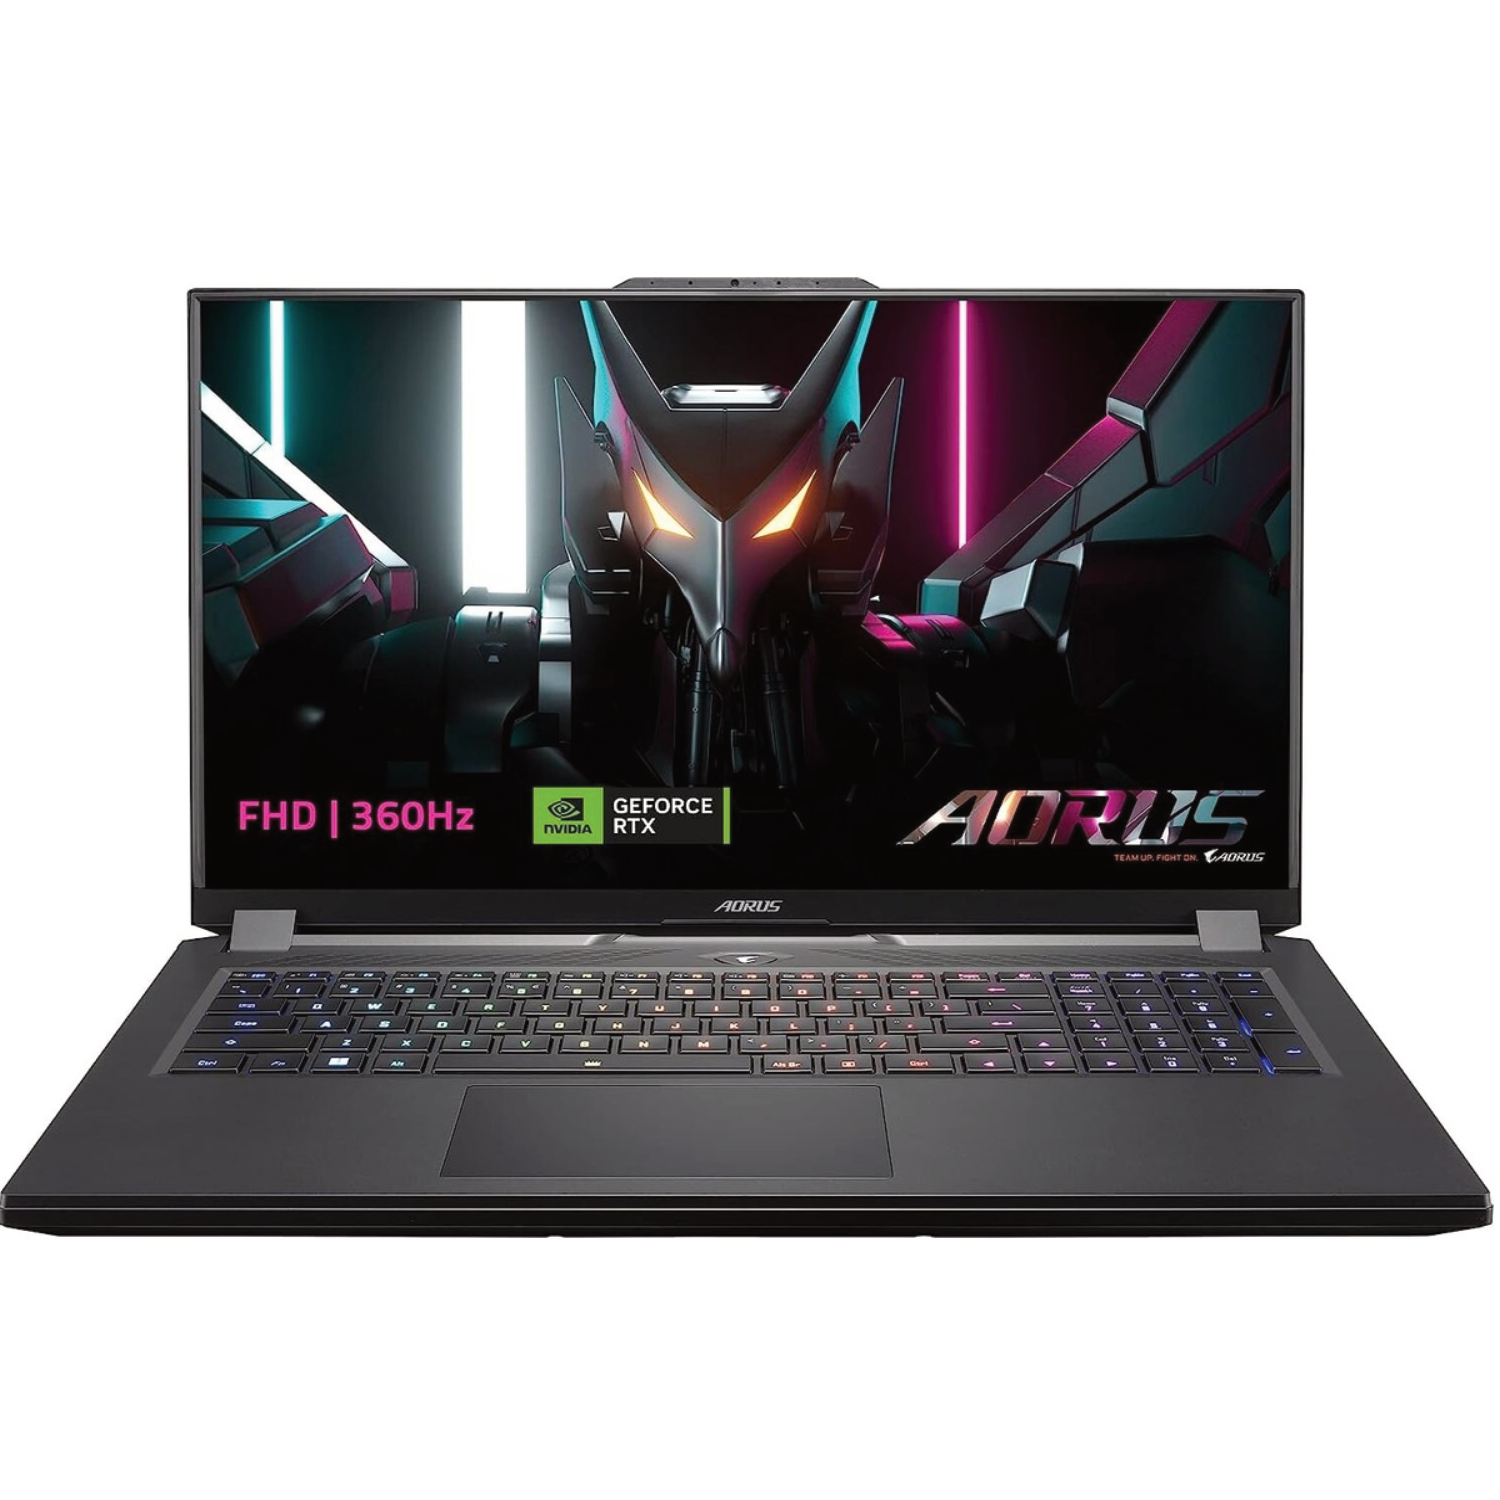
\includegraphics[height=2.5cm,keepaspectratio]{figures/Gigabyte_Aorus.png}\vspace{\fill} &
Gigabyte Aorus 7 9KF &
Processor : 12th Gen Intel(R) Core(TM) i5-12500H (2.50 GHz)

Ram : 16,0 GB

Système d'exploitation : Windows 11 Pro

Carte graphique : NVIDIA GeForce RTX 4060 Laptop GPU (8 GB) \\ \hline

\vspace{\fill}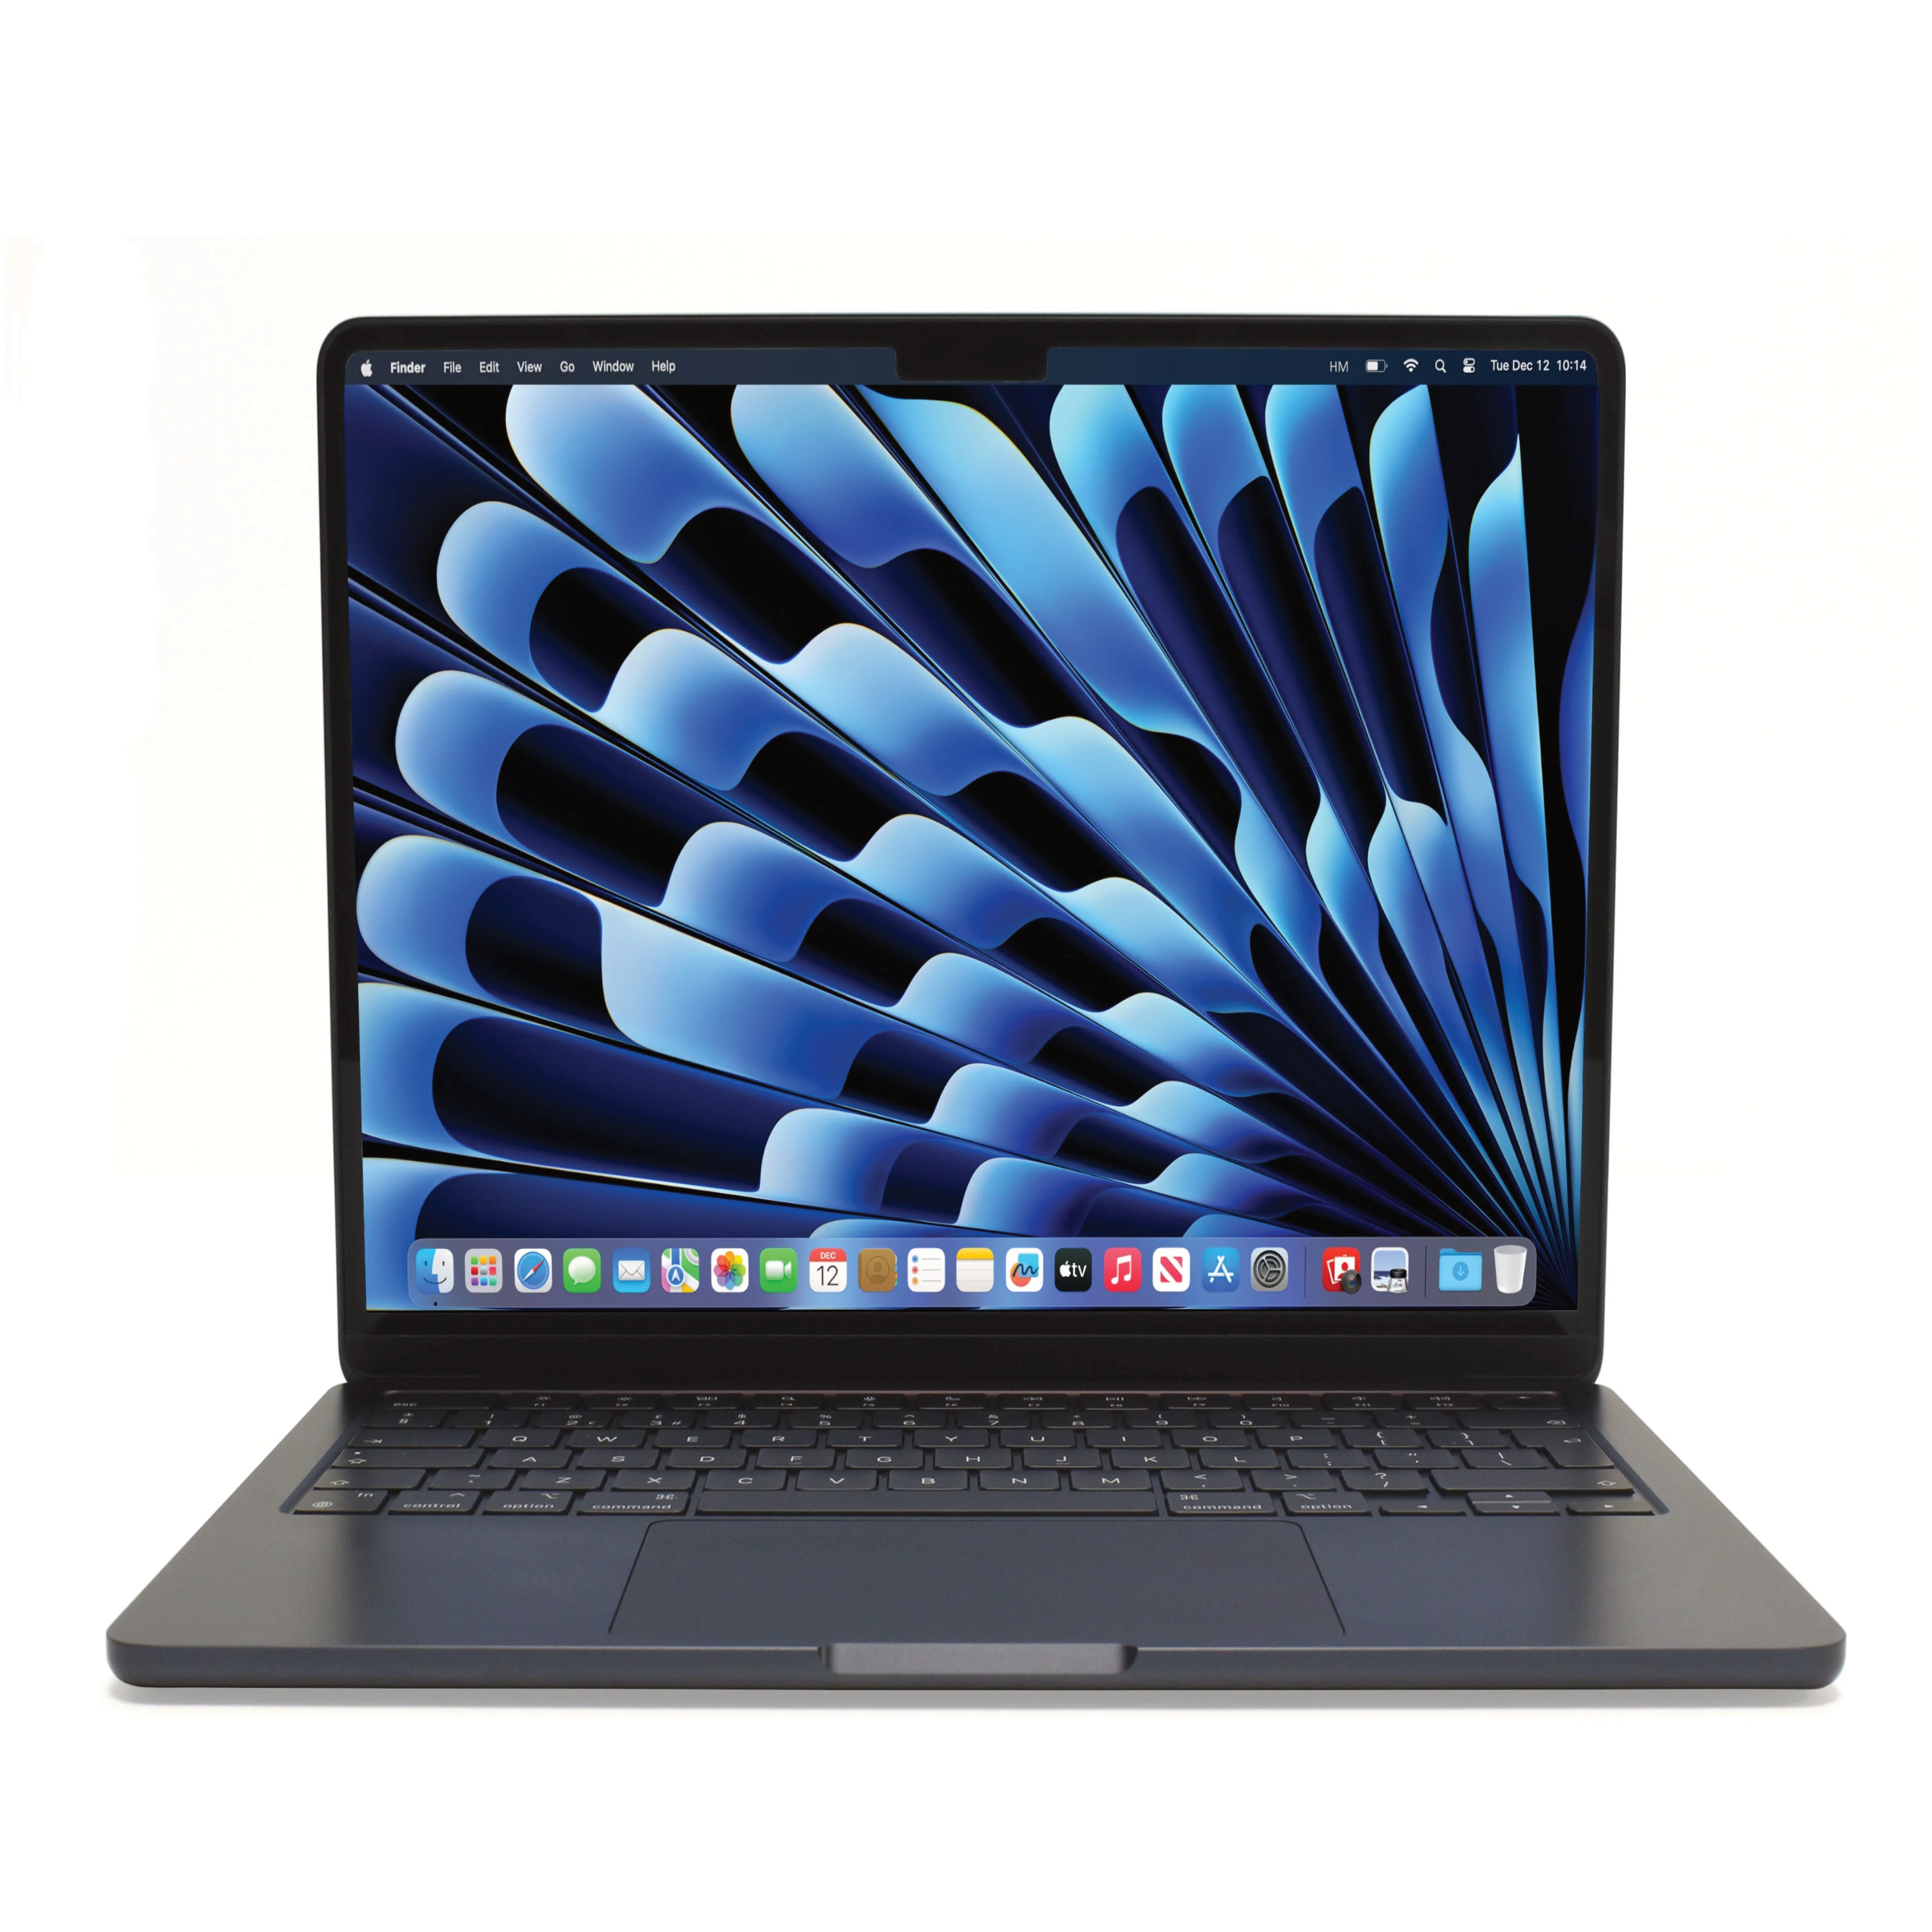
\includegraphics[height=2.5cm,keepaspectratio]{figures/macbook_air.png}\vspace{\fill} &
MacBook Air M2 &
Processor : Apple M2

Ram : 8,0 GB

Système d'exploitation : macOS Sequoia

Carte graphique : GPU intégré \\ \hline

\vspace{\fill}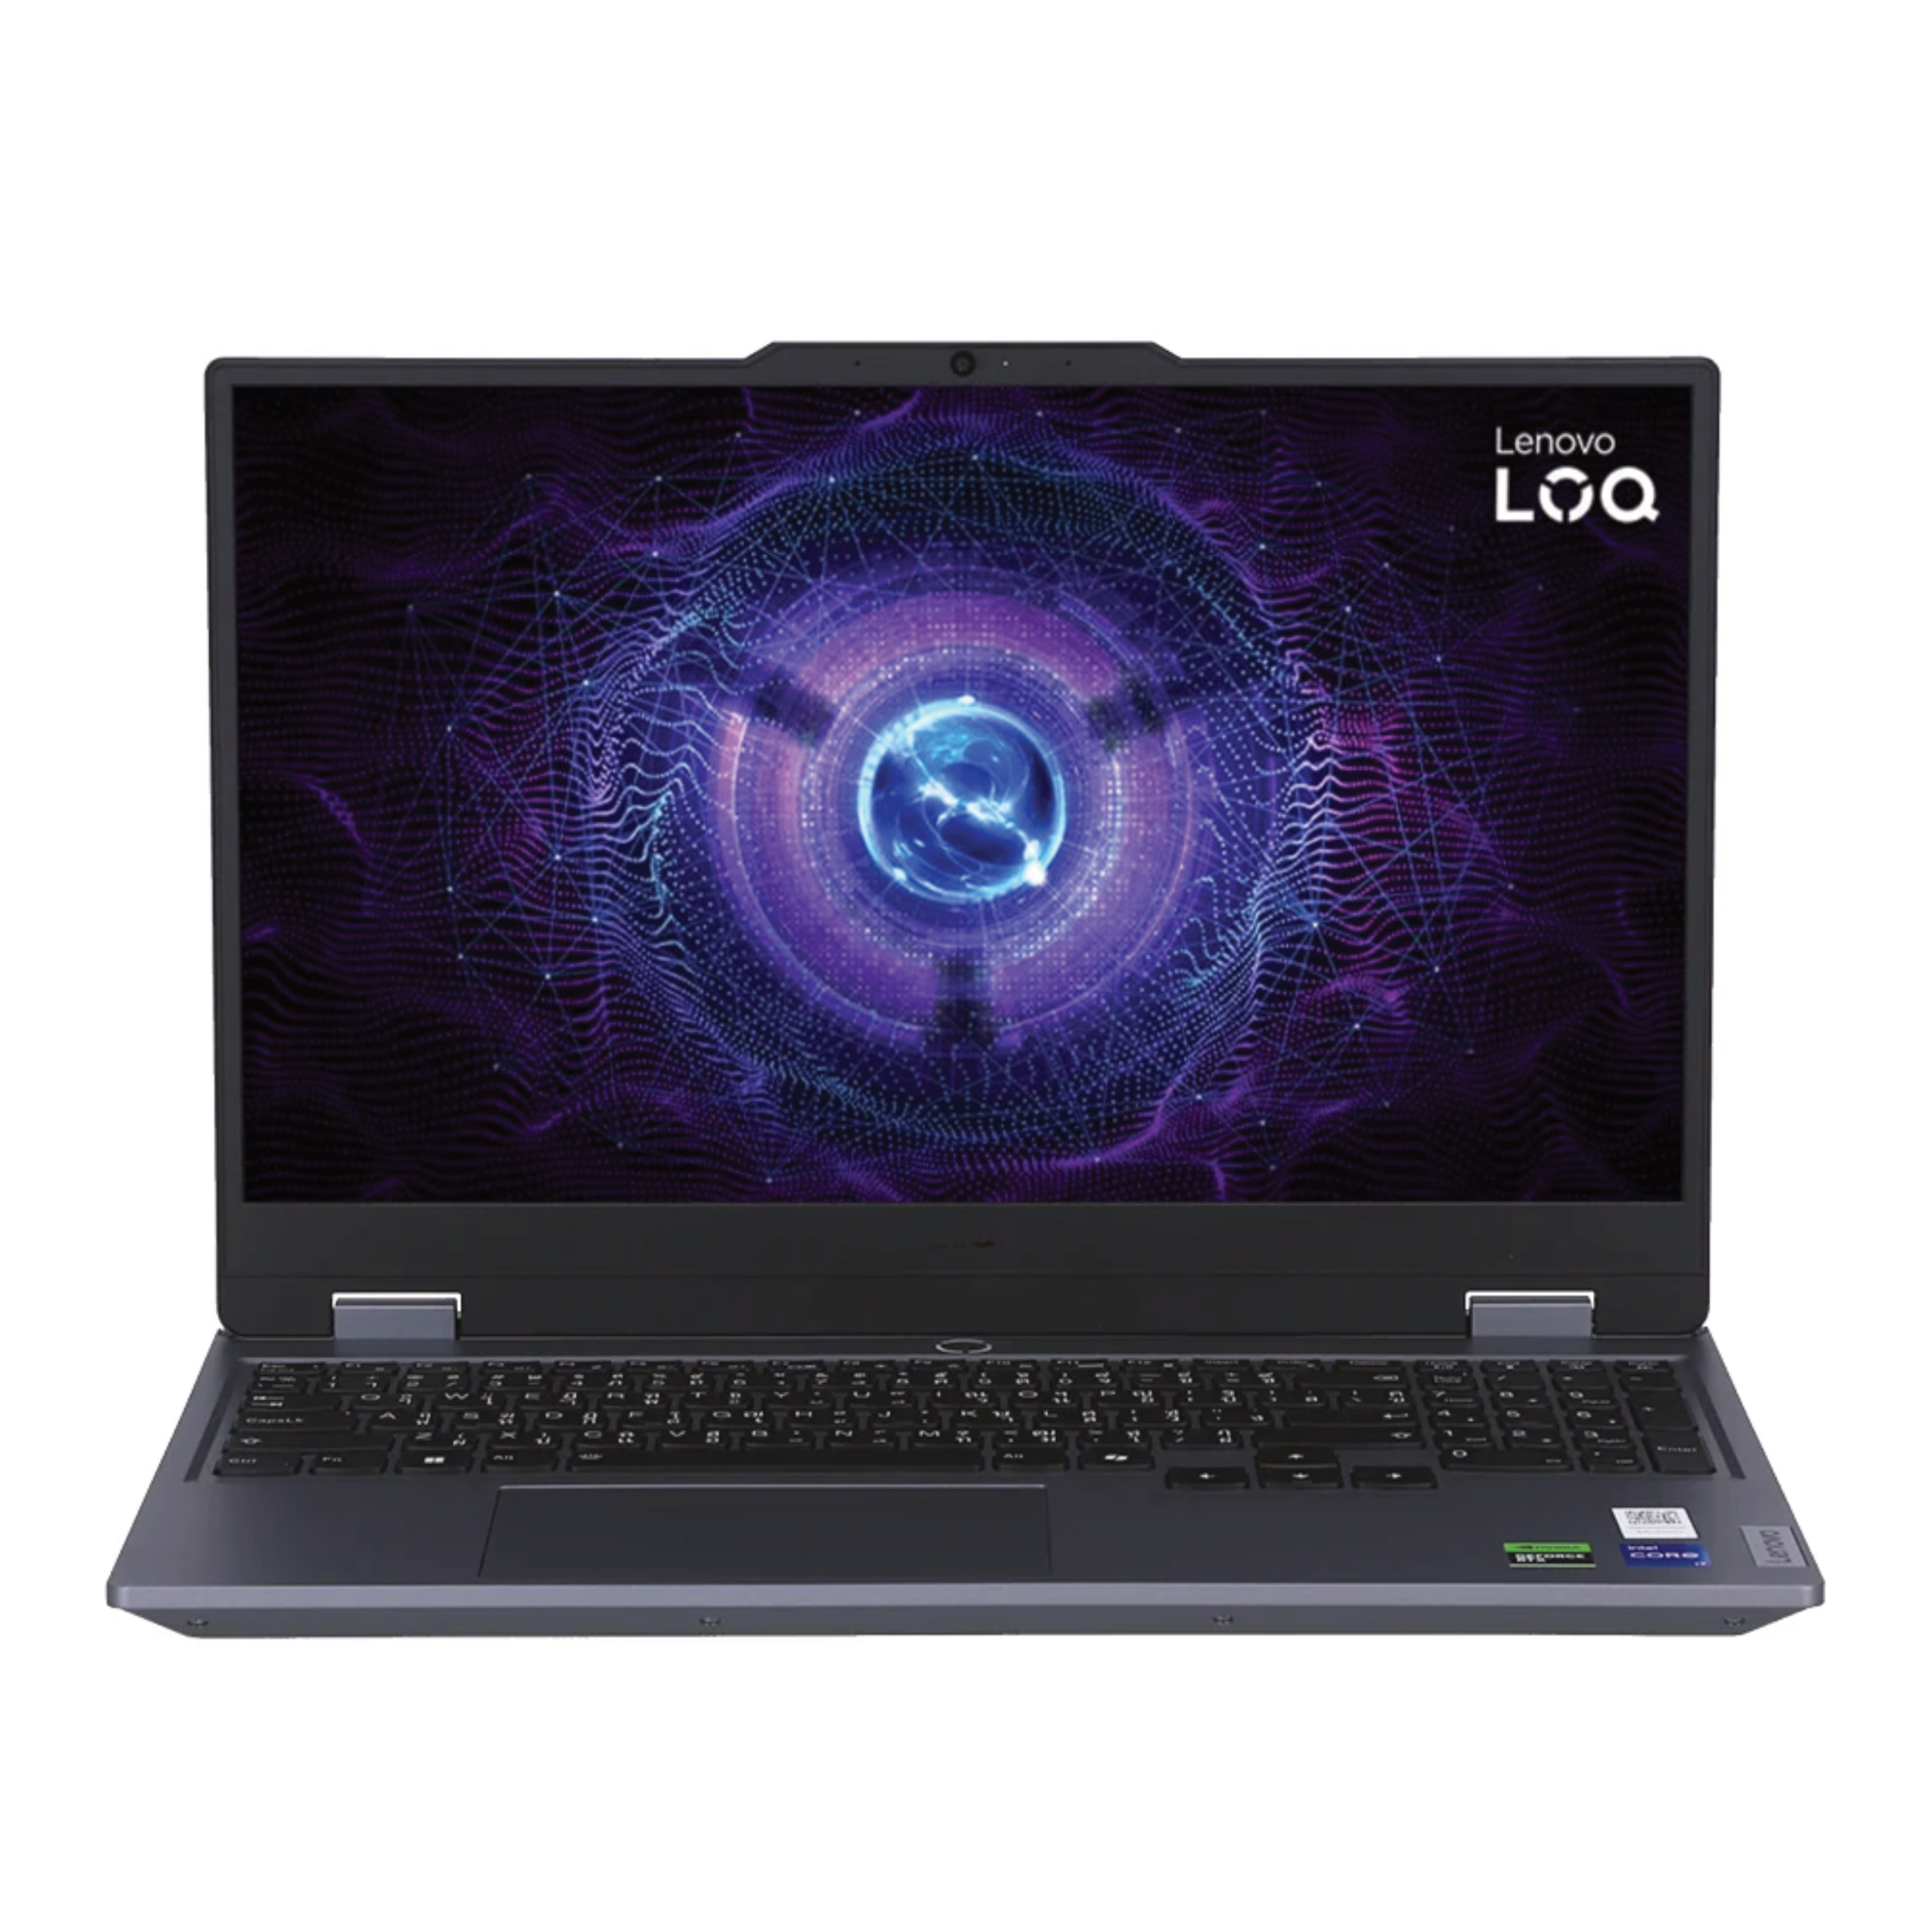
\includegraphics[height=2.5cm,keepaspectratio]{figures/Lenovo _Loq .png}\vspace{\fill} &
Lenovo Loq 15irx9 &
Processor : 13th Gen Intel(R) Core(TM) i7-13650HX (2.60 GHz)

Ram : 16,0 GB

Système d'exploitation : Windows 11 Pro

Carte graphique : NVIDIA GeForce RTX 3050 6GB Laptop GPU (6 Go) \\ \hline

\end{tabularx}
\end{table}

\subsection{Environnement logiciel}

Afin d'assurer le développement et le test efficaces de notre solution, nous avons utilisé un ensemble d'outils, de technologies et d'environnements adaptés aux besoins du projet. Cette section présente les principaux logiciels, bibliothèques et environnements de développement mobilisés tout au long de la réalisation du projet.

\subsubsection{Environnement de développement intégré:}

\subsubsection*{Visual Studio Code}

Visual Studio Code est un éditeur de code open source, gratuit et multiplateforme développé par Microsoft pour Windows, macOS et Linux. Il prend en charge plusieurs langages et technologies de développement, notamment JavaScript, TypeScript, Python, Java, C++, HTML et CSS, grâce à un vaste écosystème d'extensions. Il offre également des fonctionnalités avancées, telles que le débogage, l'intégration avec Git et diverses options de personnalisation, à travers une interface intuitive et ergonomique.

\begin{figure}[H]
	\centering
	
\includegraphics[width=0.25\textwidth]{figures/VSC.png}
	\caption{Logo de Visual Studio Code}
\end{figure}

\subsubsection*{GitHub}

GitHub est une plateforme de développement collaborative basée sur Git, permettant l'hébergement, la gestion et le partage de code source. Elle facilite le travail en équipe grâce au contrôle de version, à la gestion des branches et aux outils de collaboration tels que les pull-requests et le suivi des issues.

\begin{figure}[H]
	\centering
	
\includegraphics[width=0.25\textwidth]{figures/github.png}
	\caption{Logo de GitHub}
\end{figure}

\section{Technologies et langages de programmation utilisés}

Ce volet présente les principales technologies et langages de programmation utilisés dans le développement de la plateforme.
\subsection{Technologies de développement côté client}

Cette section présente les principales technologies utilisées pour le développement de la partie cliente de la plateforme.
\subsubsection{Angular}

Angular est un framework open source développé par Google, destiné à la création d'applications web côté client. Basé sur TypeScript, il permet de développer des applications robustes, évolutives et facilement maintenables.

\begin{figure}[H]
	\centering
	
\includegraphics[width=0.35\textwidth]{figures/angulair.png}
	\caption{Logo de Angular}
\end{figure}

\subsection{Technologies de développement côté serveur}

Cette section présente les technologies utilisées pour le développement de la partie serveur de la plateforme. 

\subsubsection{Python}

Python est un langage de programmation largement utilisé dans les domaines de la science des données, de l'analyse de données et de l'intelligence artificielle. Il se distingue par sa simplicité, sa performance et la richesse de ses bibliothèques dédiées au traitement des données textuelles et numériques, même à grande échelle. Grâce à sa flexibilité et à son vaste écosystème, Python constitue une solution adaptée aux applications de traitement et d'analyse de données.

\begin{figure}[H]
	\centering
	
\includegraphics[width=0.25\textwidth]{figures/python.png}
	\caption{Logo de Python}
\end{figure}

\subsubsection{NestJS}

NestJS est un framework open source basé sur Node.js, utilisé pour le développement d'applications serveur évolutives et maintenables. Il repose sur TypeScript et adopte une architecture modulaire inspirée d'Angular, facilitant la structuration des applications backend.

\begin{figure}[H]
	\centering
	
\includegraphics[width=0.35\textwidth]{figures/nest.png}
	\caption{Logo de NestJS}
\end{figure}

\subsubsection{Node.js}

Node.js est une plateforme logicielle open source basée sur JavaScript, conçue pour le développement d'applications réseau évolutives et fortement concurrentes, reposant sur un modèle orienté événements. Elle permet de construire des applications performantes capables de gérer un grand nombre de connexions simultanées.

\begin{figure}[H]
	\centering
	
\includegraphics[width=0.35\textwidth]{figures/node.png}
	\caption{Logo de Node.js}
\end{figure}

\subsection{Technologies de gestion des données}
Cette partie présente les technologies utilisées pour la gestion, le stockage et la manipulation des données au sein de la plateforme.
\subsubsection{MongoDB}

MongoDB est une base de données NoSQL orientée documents, conçue pour stocker et gérer des données de manière flexible et scalable. Elle utilise un format similaire au JSON (BSON), ce qui facilite le stockage de données non structurées et leur exploitation dans des applications modernes.

\begin{figure}[H]
	\centering
	
\includegraphics[width=0.35\textwidth]{figures/mongo.png}
	\caption{Logo de MongoDB}
\end{figure}

\subsubsection{PostgreSQL}

PostgreSQL est un système de gestion de bases de données relationnelles objet open source, reconnu pour sa fiabilité, son intégrité des données, ses fonctionnalités avancées et sa conformité aux standards SQL.

\begin{figure}[H]
	\centering
	
\includegraphics[width=0.25\textwidth]{figures/PostgreSQL .png}
	\caption{Logo de PostgreSQL}
\end{figure}

\subsubsection{Supabase}

Supabase est une plateforme open source de type Backend-as-a-Service (BaaS) qui fournit des services prêts à l'emploi tels qu'une base de données PostgreSQL, l'authentification, le stockage et des API automatiques pour faciliter le développement d'applications web et mobiles.

\begin{figure}[H]
	\centering
	
\includegraphics[width=0.35\textwidth]{figures/supabase.png}
	\caption{Logo de Supabase}
\end{figure}

\subsection{Outil de conception et de modélisation}
Cette partie présente l’outil utilisé pour la conception et la modélisation du système. 

\subsubsection{Draw.io}

Draw.io est un logiciel de diagramme en ligne gratuit permettant de concevoir différents types de schémas, notamment des diagrammes UML, des diagrammes de processus, des modèles entités-associations, des organigrammes et des diagrammes de réseau. Il est largement utilisé pour la modélisation et la documentation des systèmes informatiques.

\begin{figure}[H]
	\centering
	
\includegraphics[width=0.25\textwidth]{figures/digrammes.png}
	\caption{Logo de Draw.io}
\end{figure}

\subsection{Service d'intelligence artificielle}
Cette partie présente le service d’intelligence artificielle intégré à la plateforme. 

\subsubsection{Gemini API}

Gemini API est une interface de programmation proposée par Google permettant d'accéder aux modèles d'intelligence artificielle Gemini. Elle offre des fonctionnalités de génération de texte, d'analyse de contenu et de compréhension multimodale (texte, image, etc.), facilitant leur intégration dans des applications.

\begin{figure}[H]
	\centering
	
\includegraphics[width=0.35\textwidth]{figures/gemini.png}
	\caption{Logo de Gemini API}
\end{figure}

\section{Principales interfaces graphiques}

Cette section est dédiée à la présentation des interfaces graphiques développées au cours de notre projet. Ces interfaces permettent de visualiser de manière intuitive l'ensemble de nos modules fonctionnels : la génération du CV ATS, l'évaluation des scores actuels ATS et employabilité, ainsi que le score d'employabilité prévisionnel après l'obtention des certifications recommandées.

\subsection{Authentification}

La figure~\ref{fig:acces-academique-professionnel} ci-dessous illustre l'interface d'authentification de la plateforme, où l'étudiant et l'administrateur se connectent via l'accès académique, tandis que les sociétés utilisent l'accès professionnel.

\begin{figure}[H]
\centering
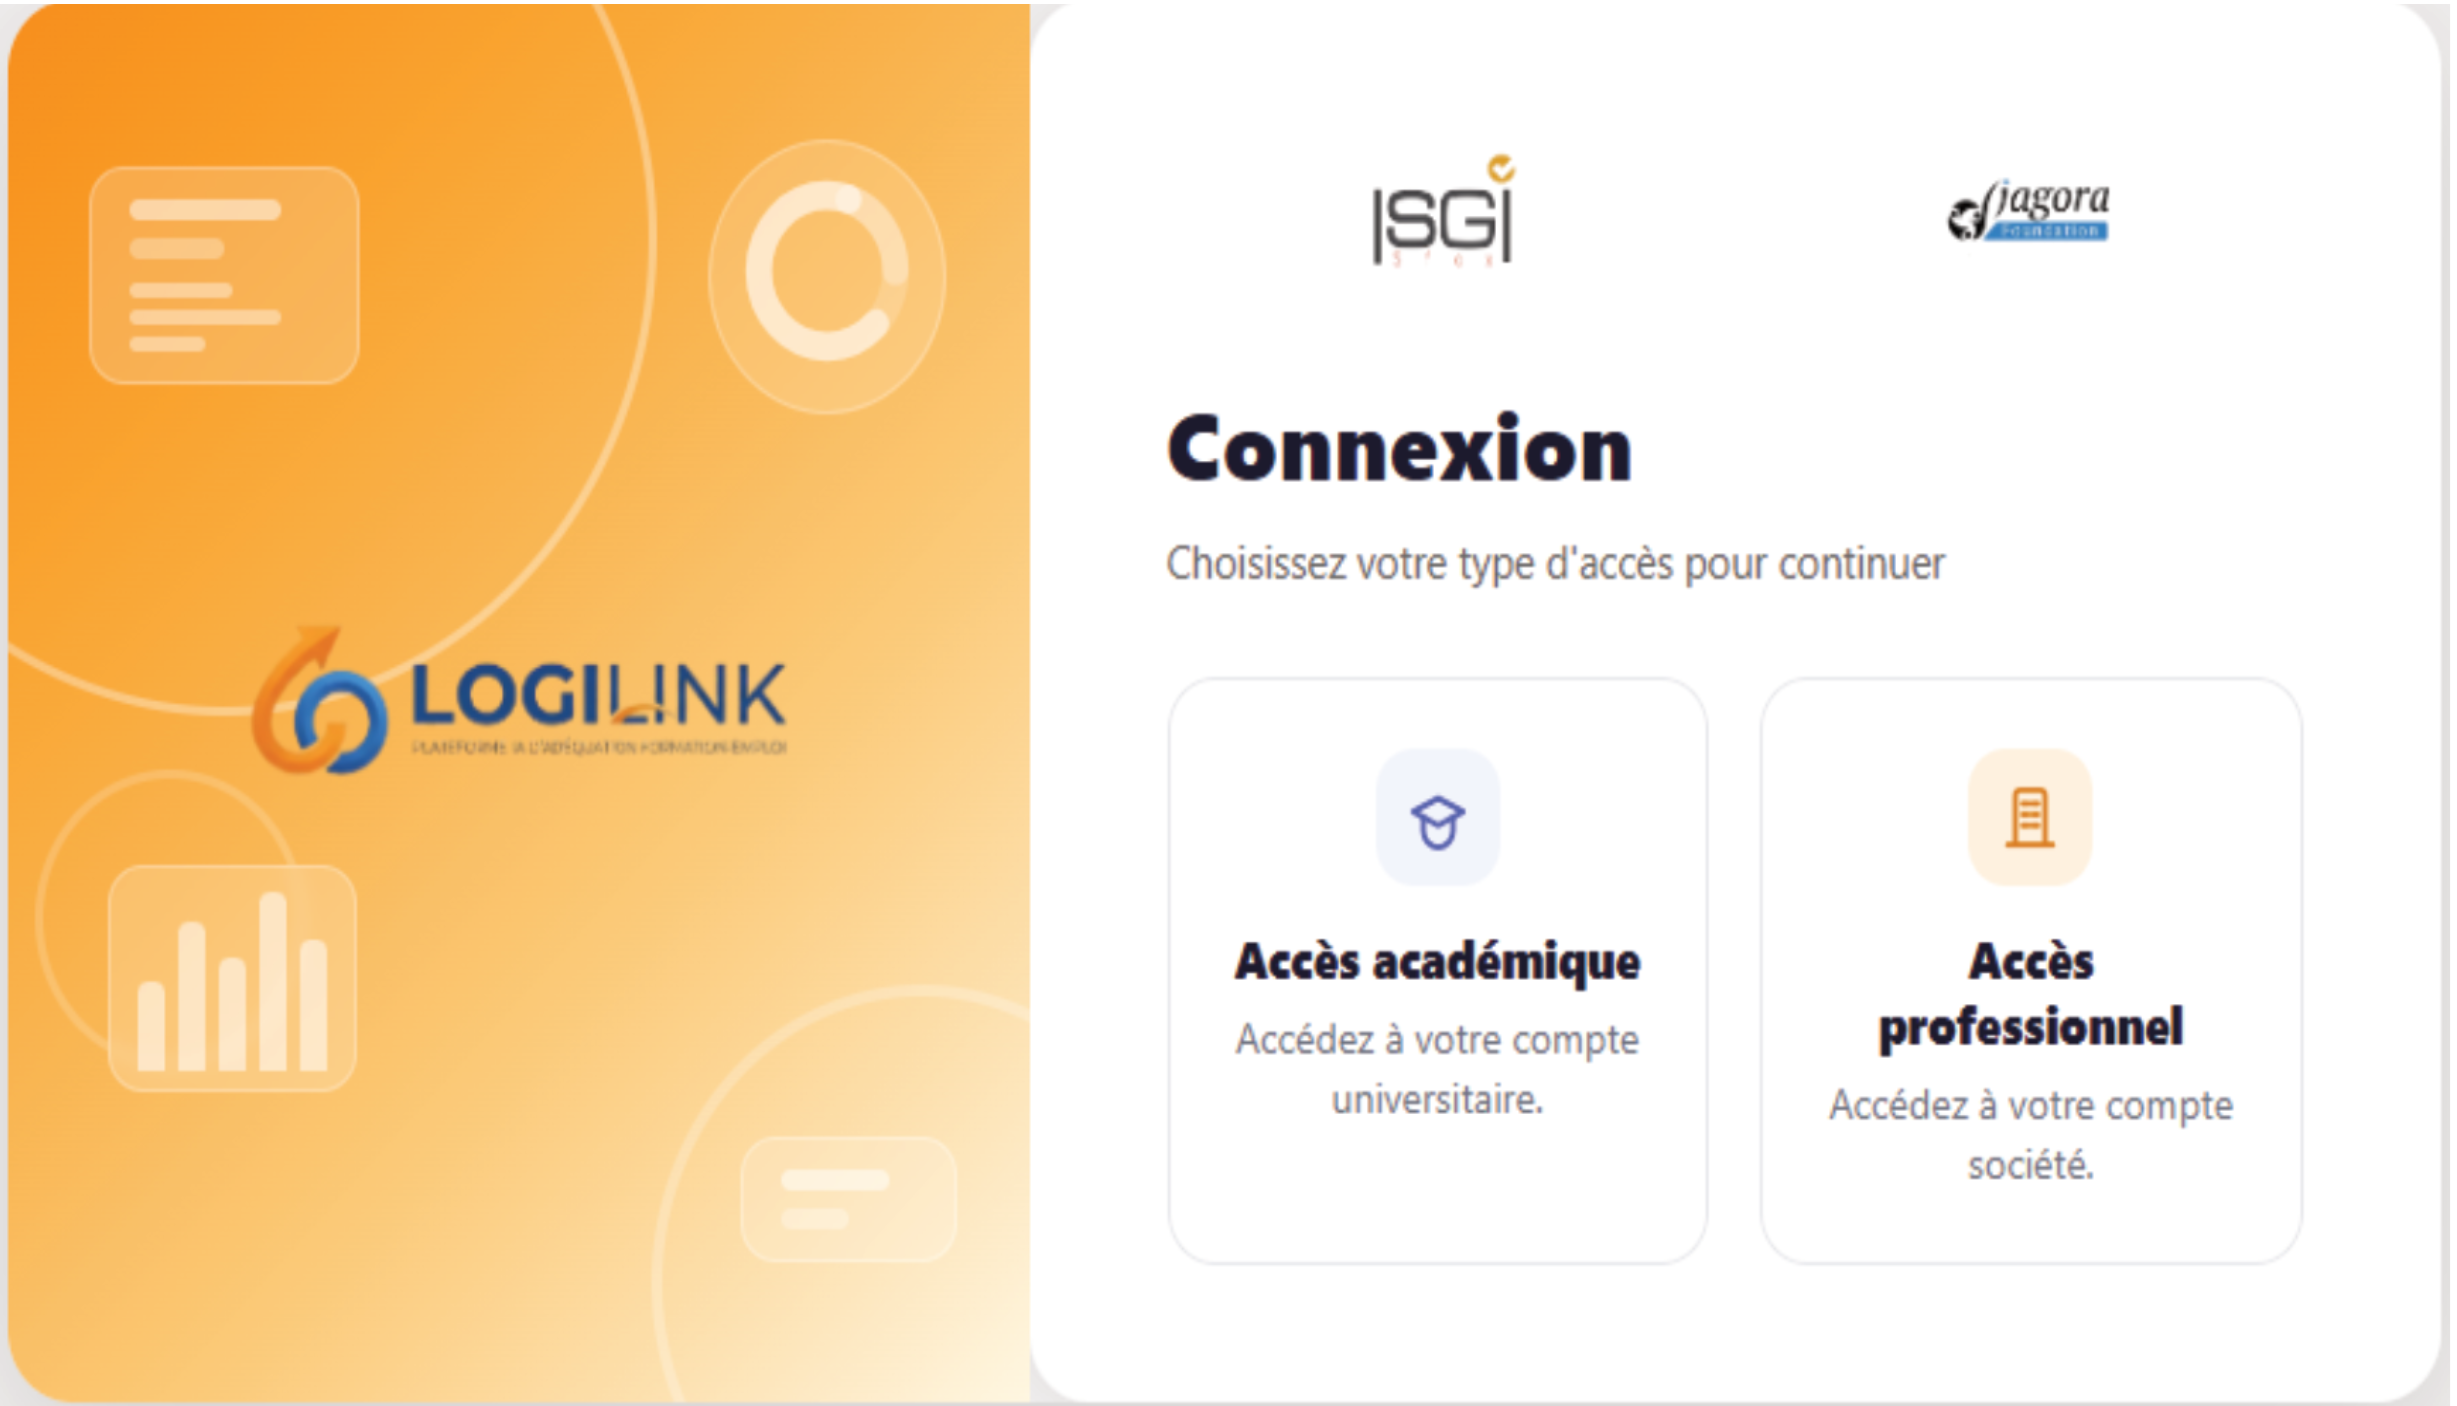
\includegraphics[width=0.85\textwidth]{figures/Interface_daacces_academique_et_professionnel.png}
\caption{Interface d'accès académique et professionnel}
\label{fig:acces-academique-professionnel}
\end{figure}

\noindent La figure~\ref{fig:authentification} indique que pour s'authentifier, l'étudiant ou l'administrateur doit simplement saisir son identifiant et son mot de passe.

\begin{figure}[H]
\centering
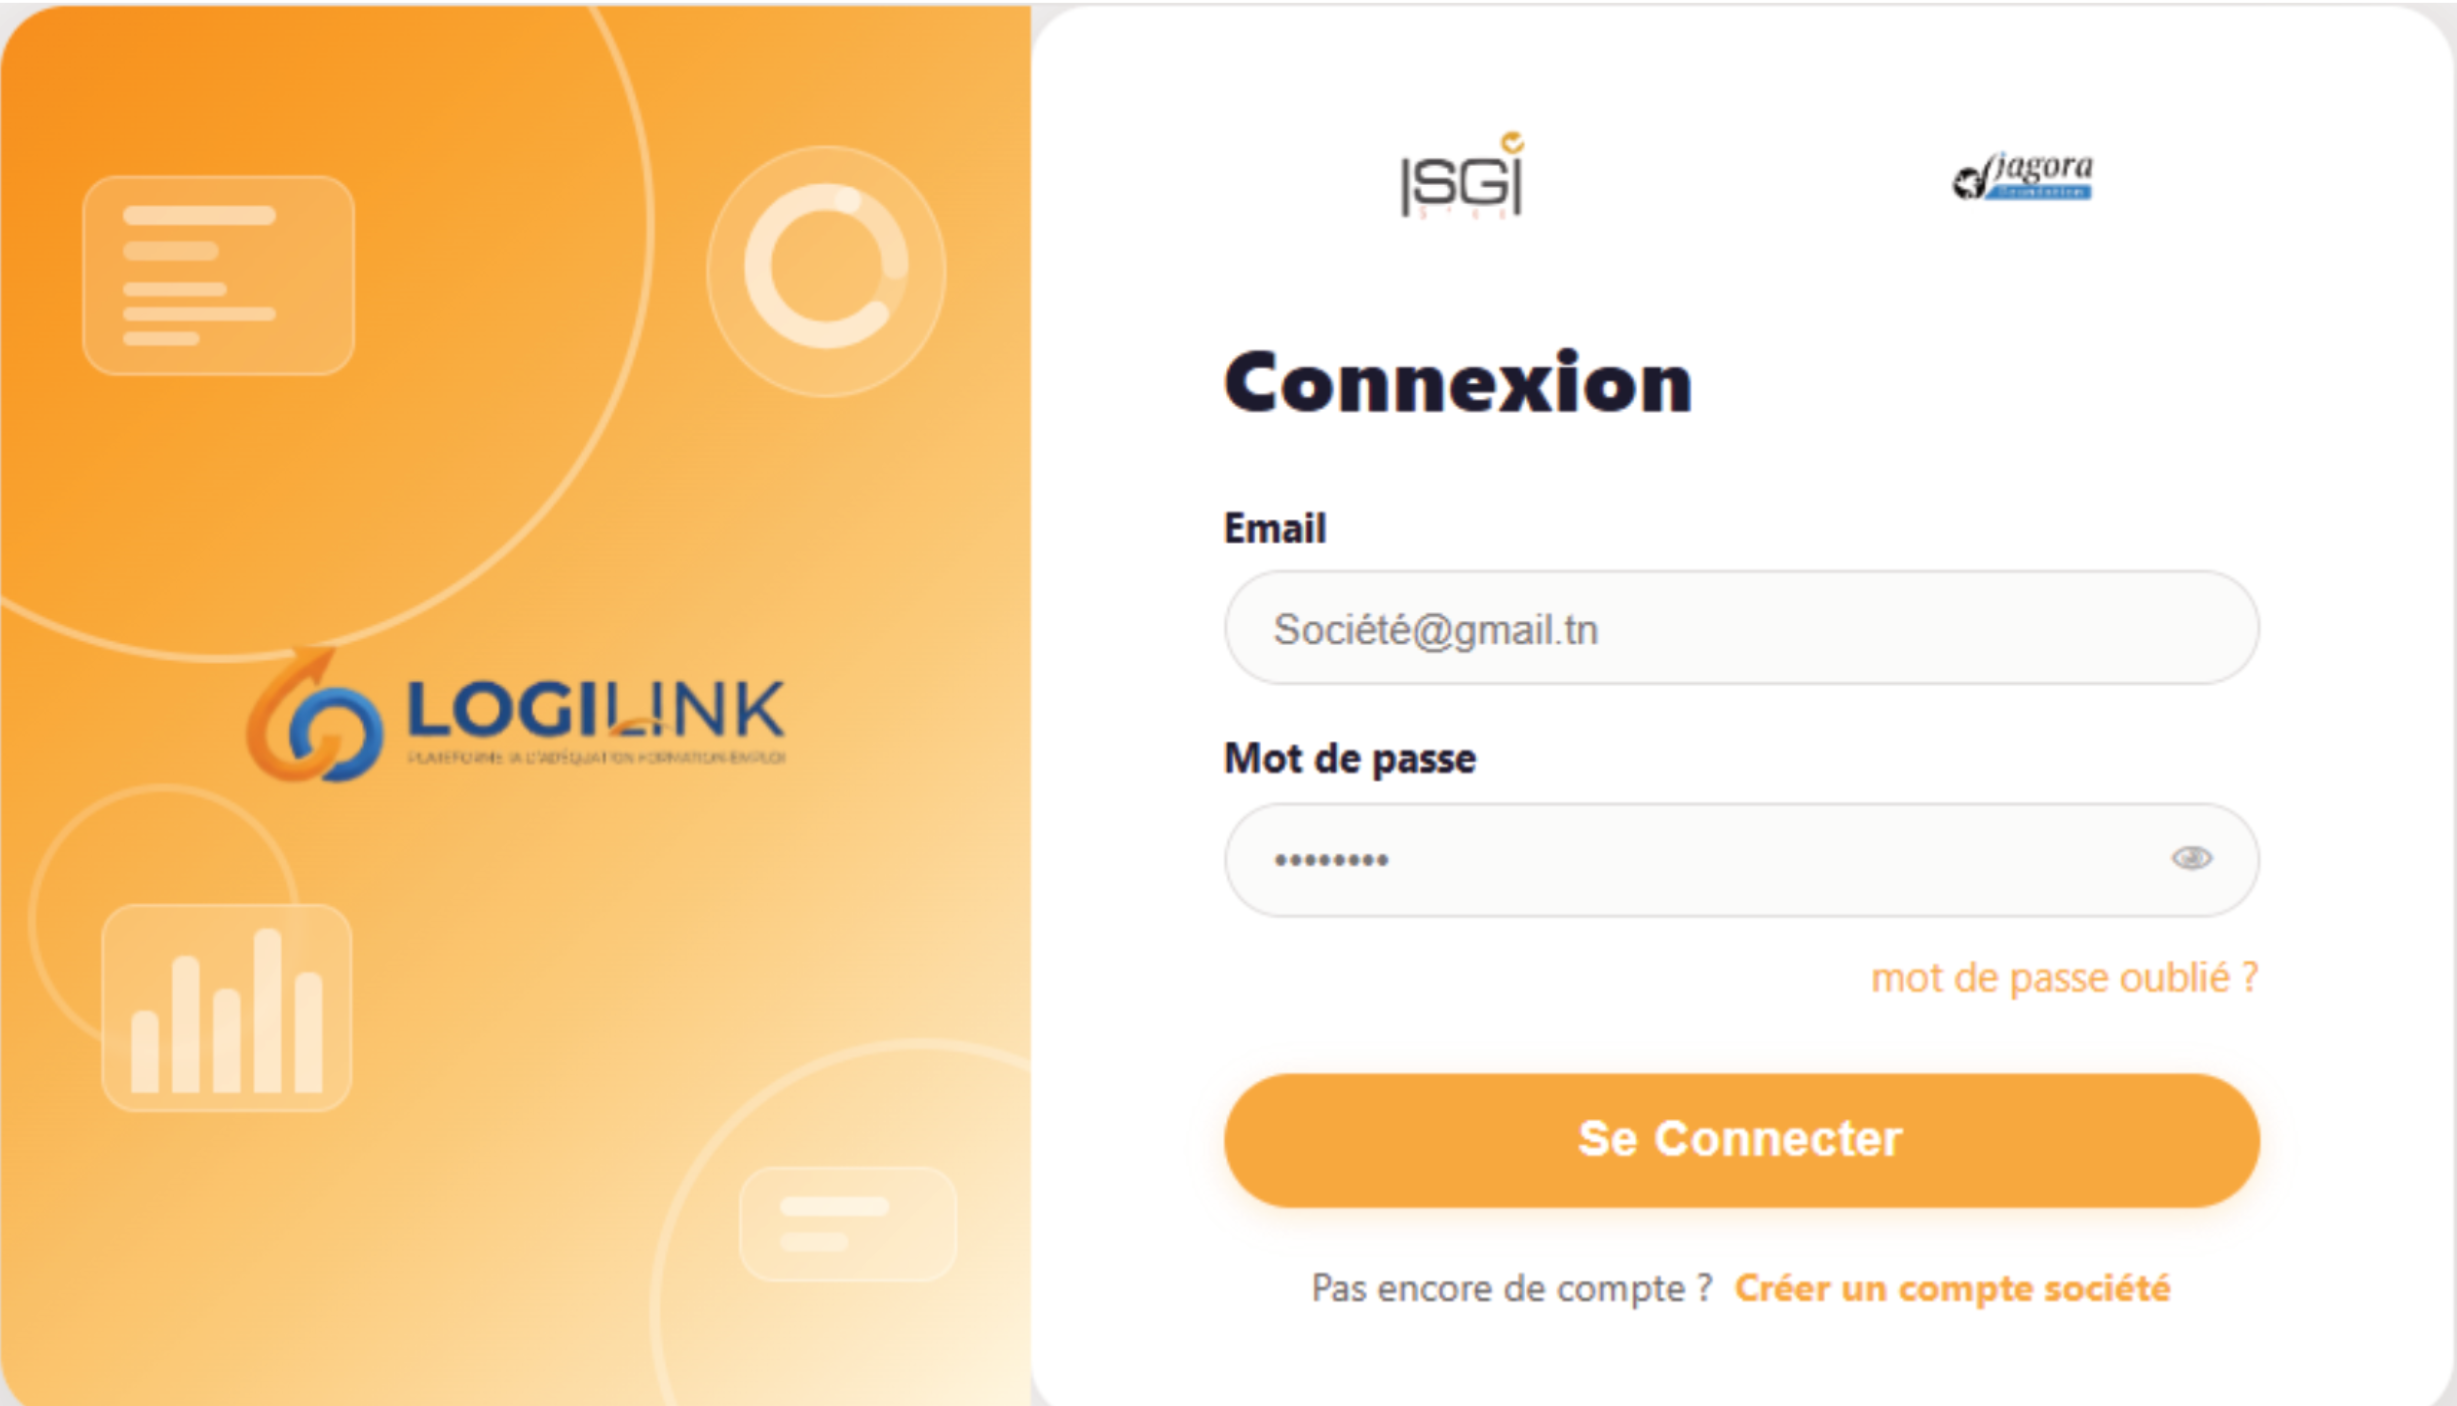
\includegraphics[width=0.85\textwidth]{figures/Interface_daauthentification.png}
\caption{Interface d'authentification}
\label{fig:authentification}
\end{figure}

\noindent La figure~\ref{fig:verification-identite} ci-dessous illustre l'étape de vérification de l'identité de l'étudiant. Après la saisie de son identifiant et de son mot de passe, un code de vérification à six chiffres est envoyé à son adresse e-mail afin de confirmer son identité.

\begin{figure}[H]
\centering
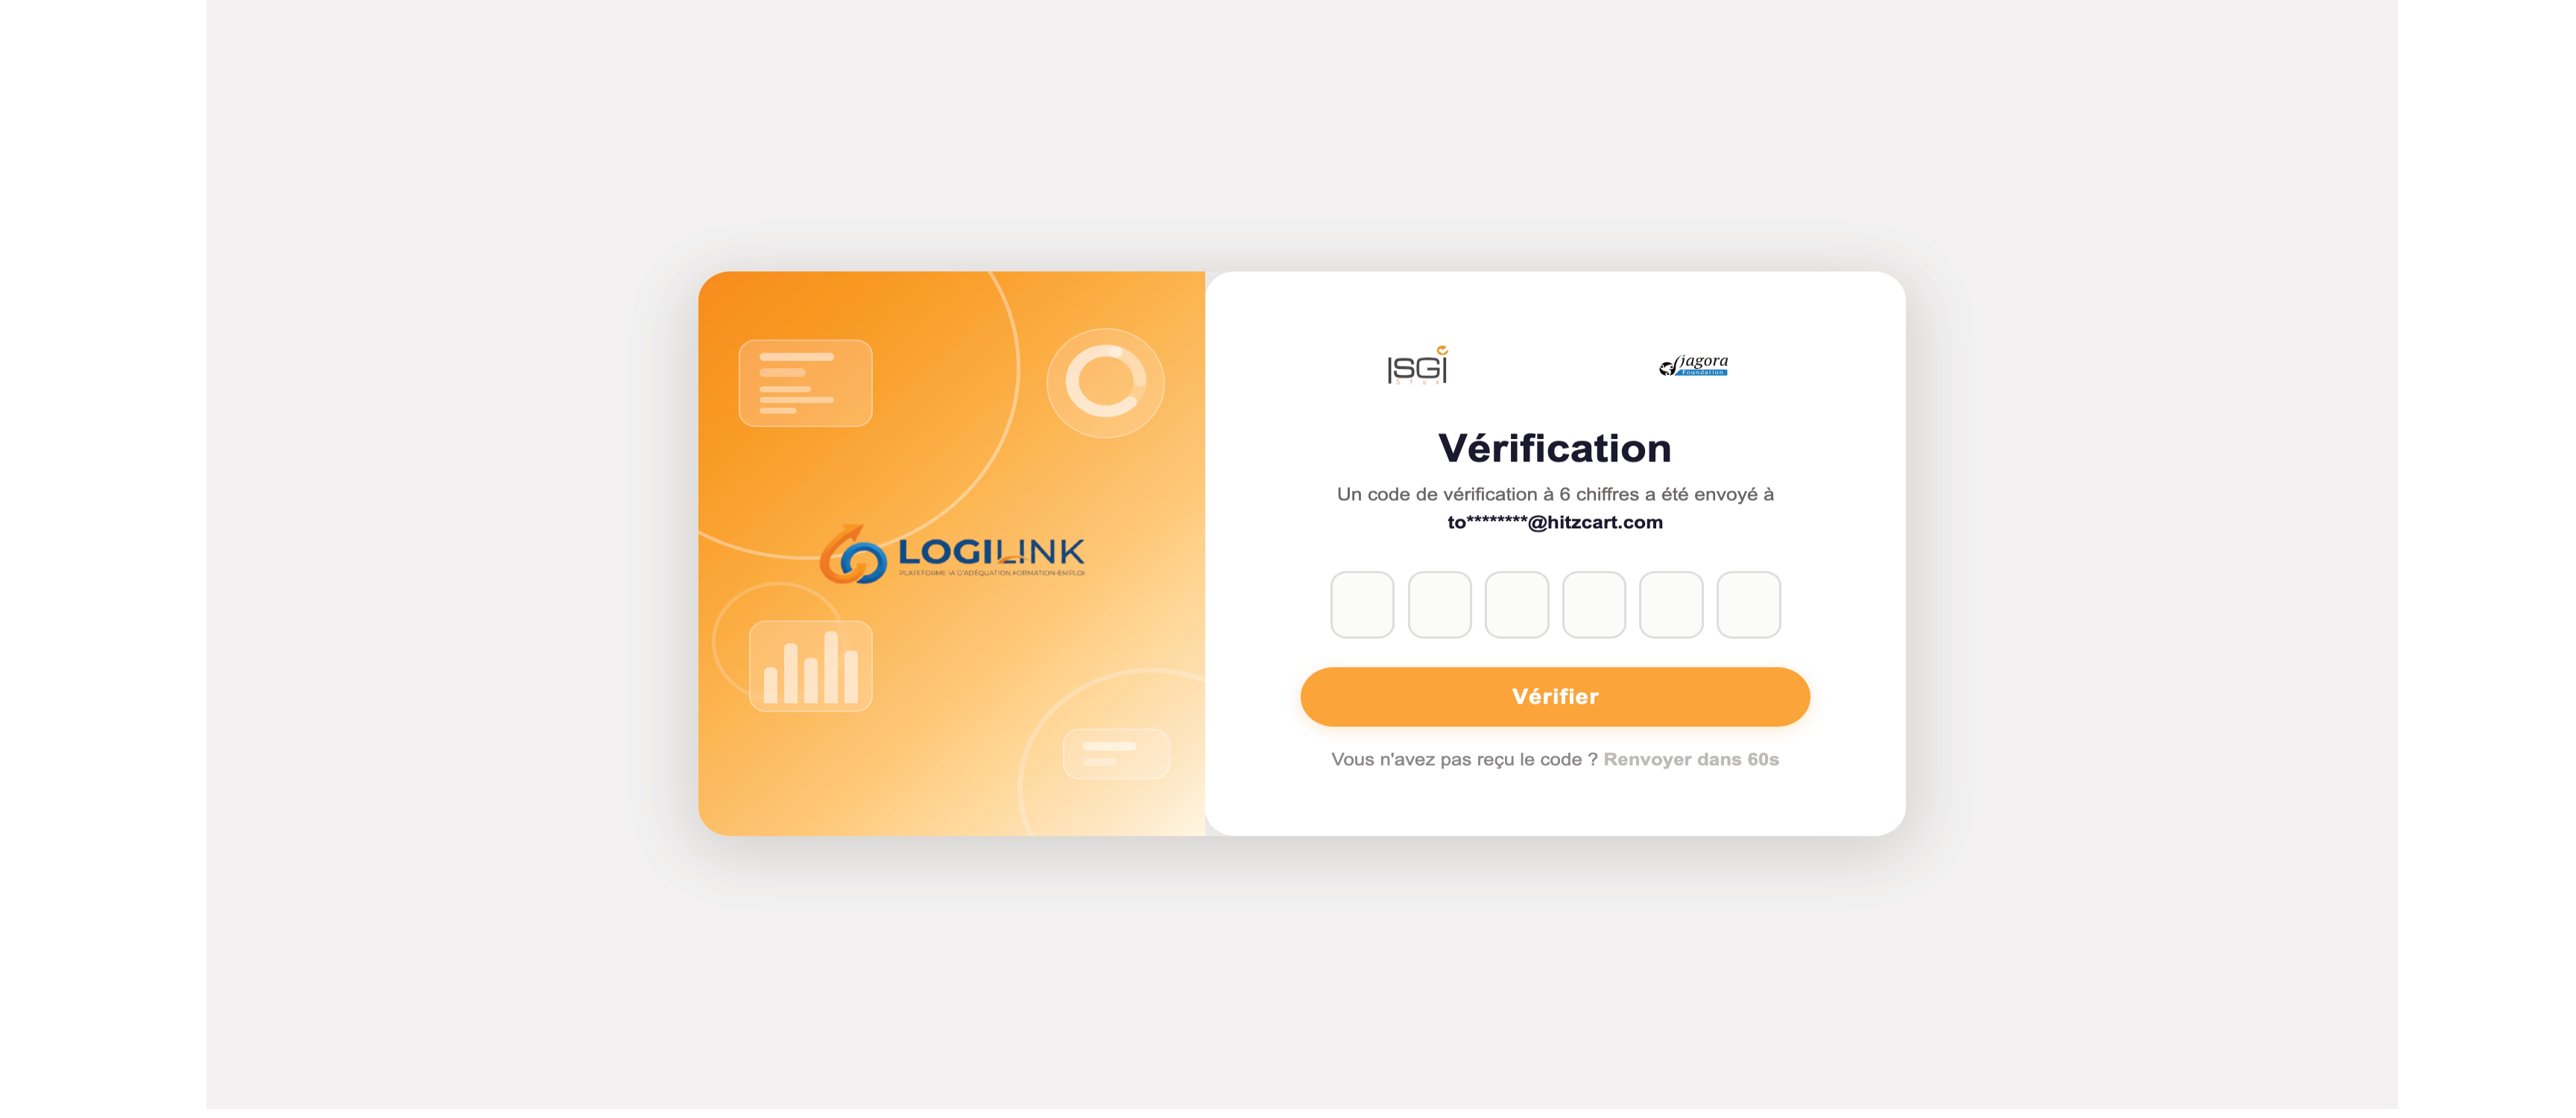
\includegraphics[width=0.85\textwidth]{figures/Interface_de_verification_daidentite.png}
\caption{Interface de vérification d'identité}
\label{fig:verification-identite}
\end{figure}

\noindent La figure~\ref{fig:creation-compte-societe} ci-dessous illustre l'interface d'inscription permettant à une société de créer un compte en renseignant ses informations professionnelles.

\begin{figure}[H]
\centering
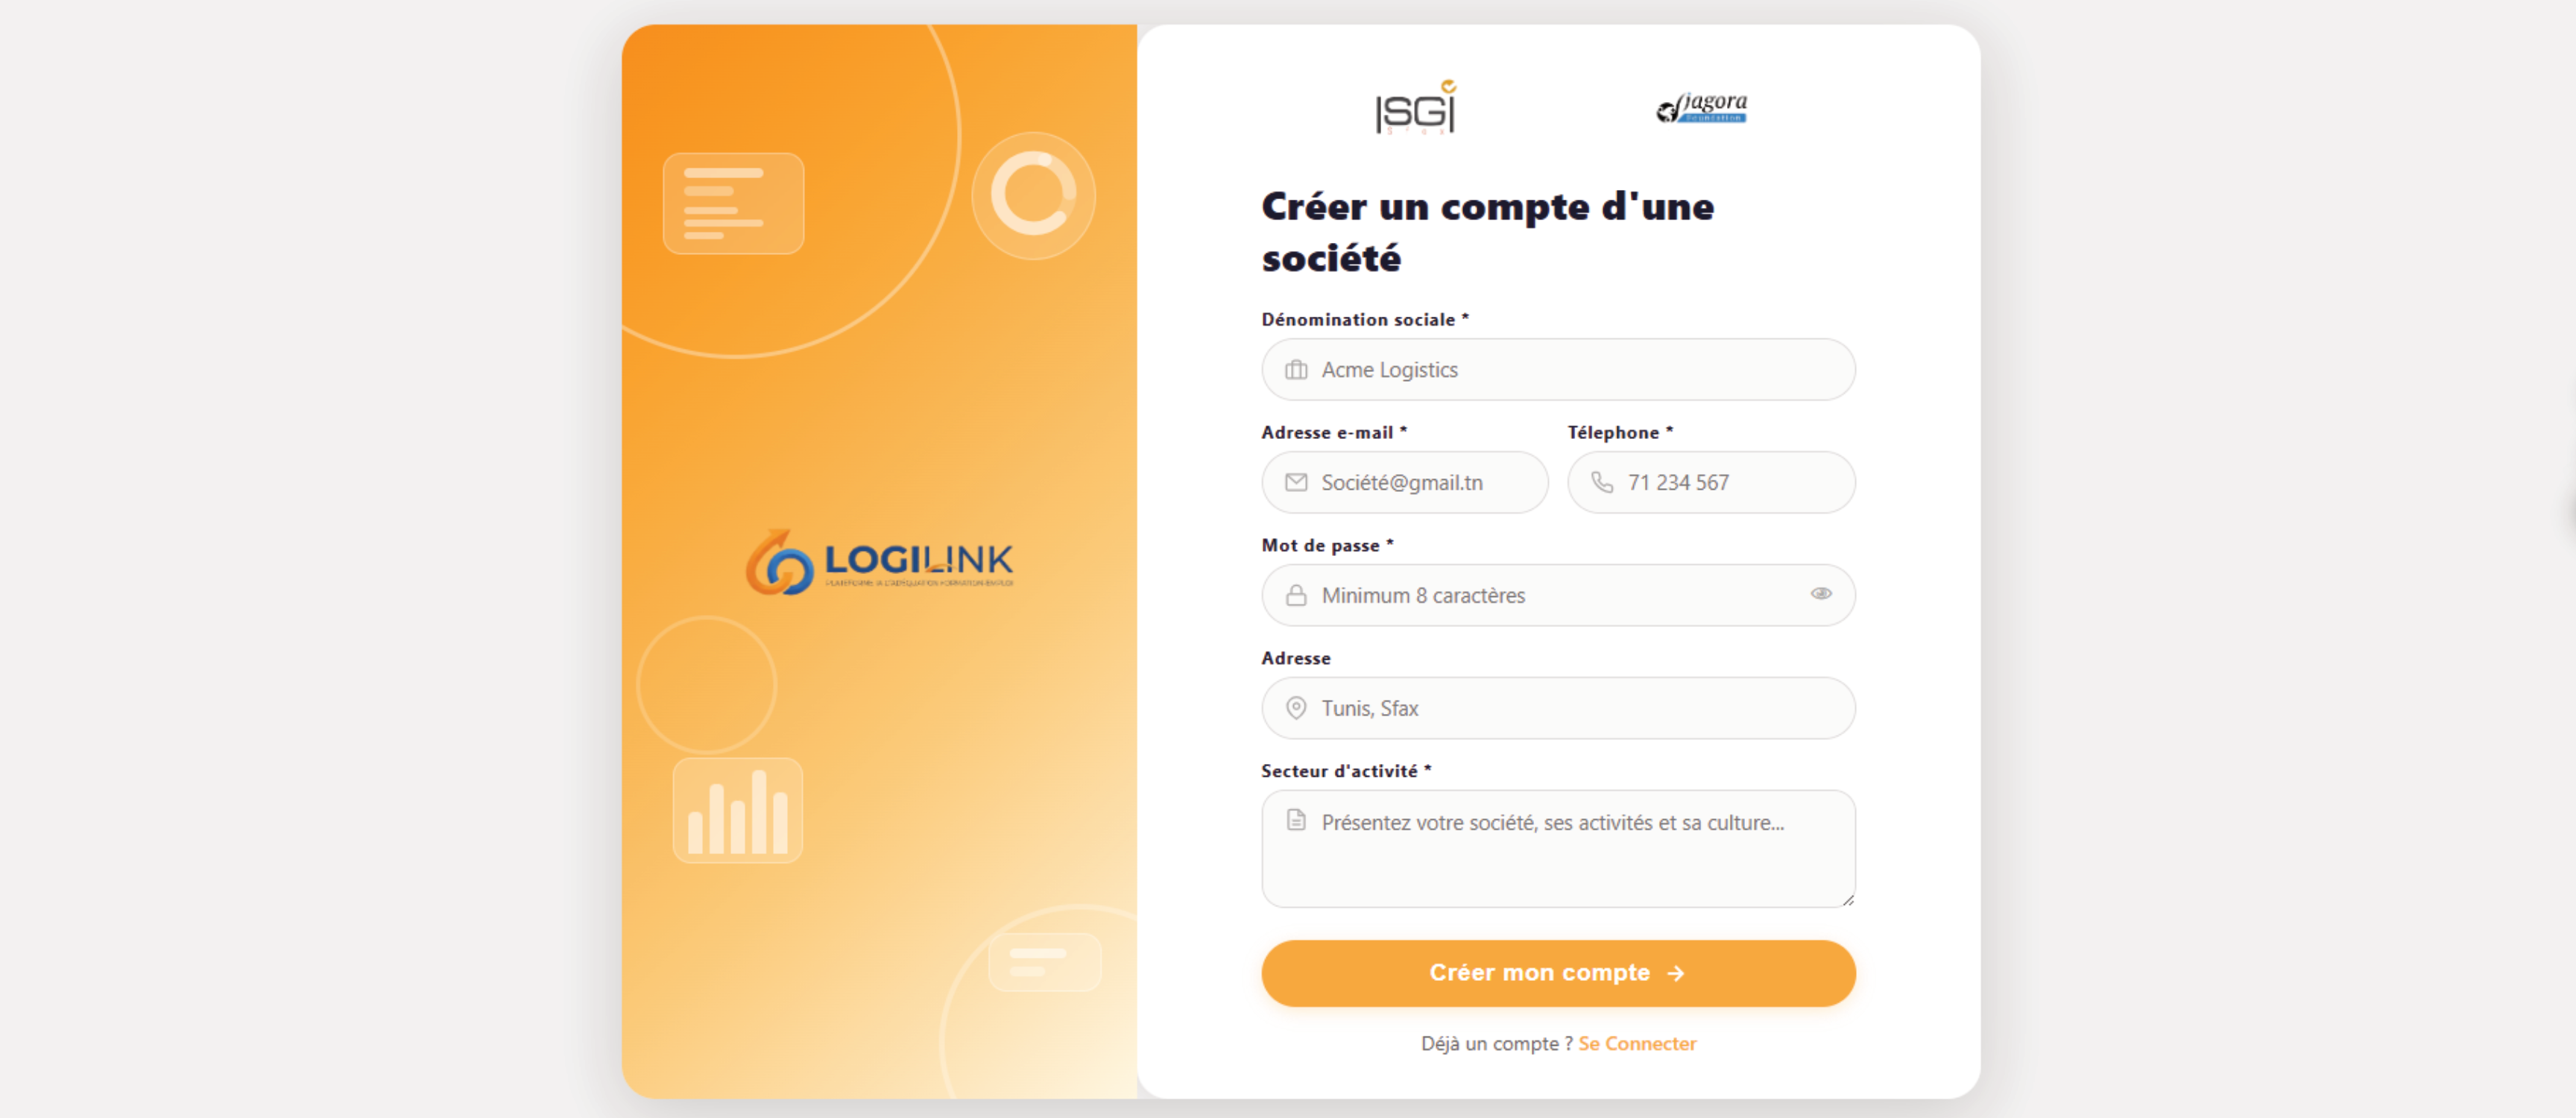
\includegraphics[width=0.85\textwidth]{figures/Interface_de_creation_de_compte_societe.png}
\caption{Interface de création de compte société}
\label{fig:creation-compte-societe}
\end{figure}

\noindent La figure~\ref{fig:authentification-societe} ci-dessous, il suffit à la société de saisir son adresse e-mail et son mot de passe pour s'authentifier.

\begin{figure}[H]
\centering
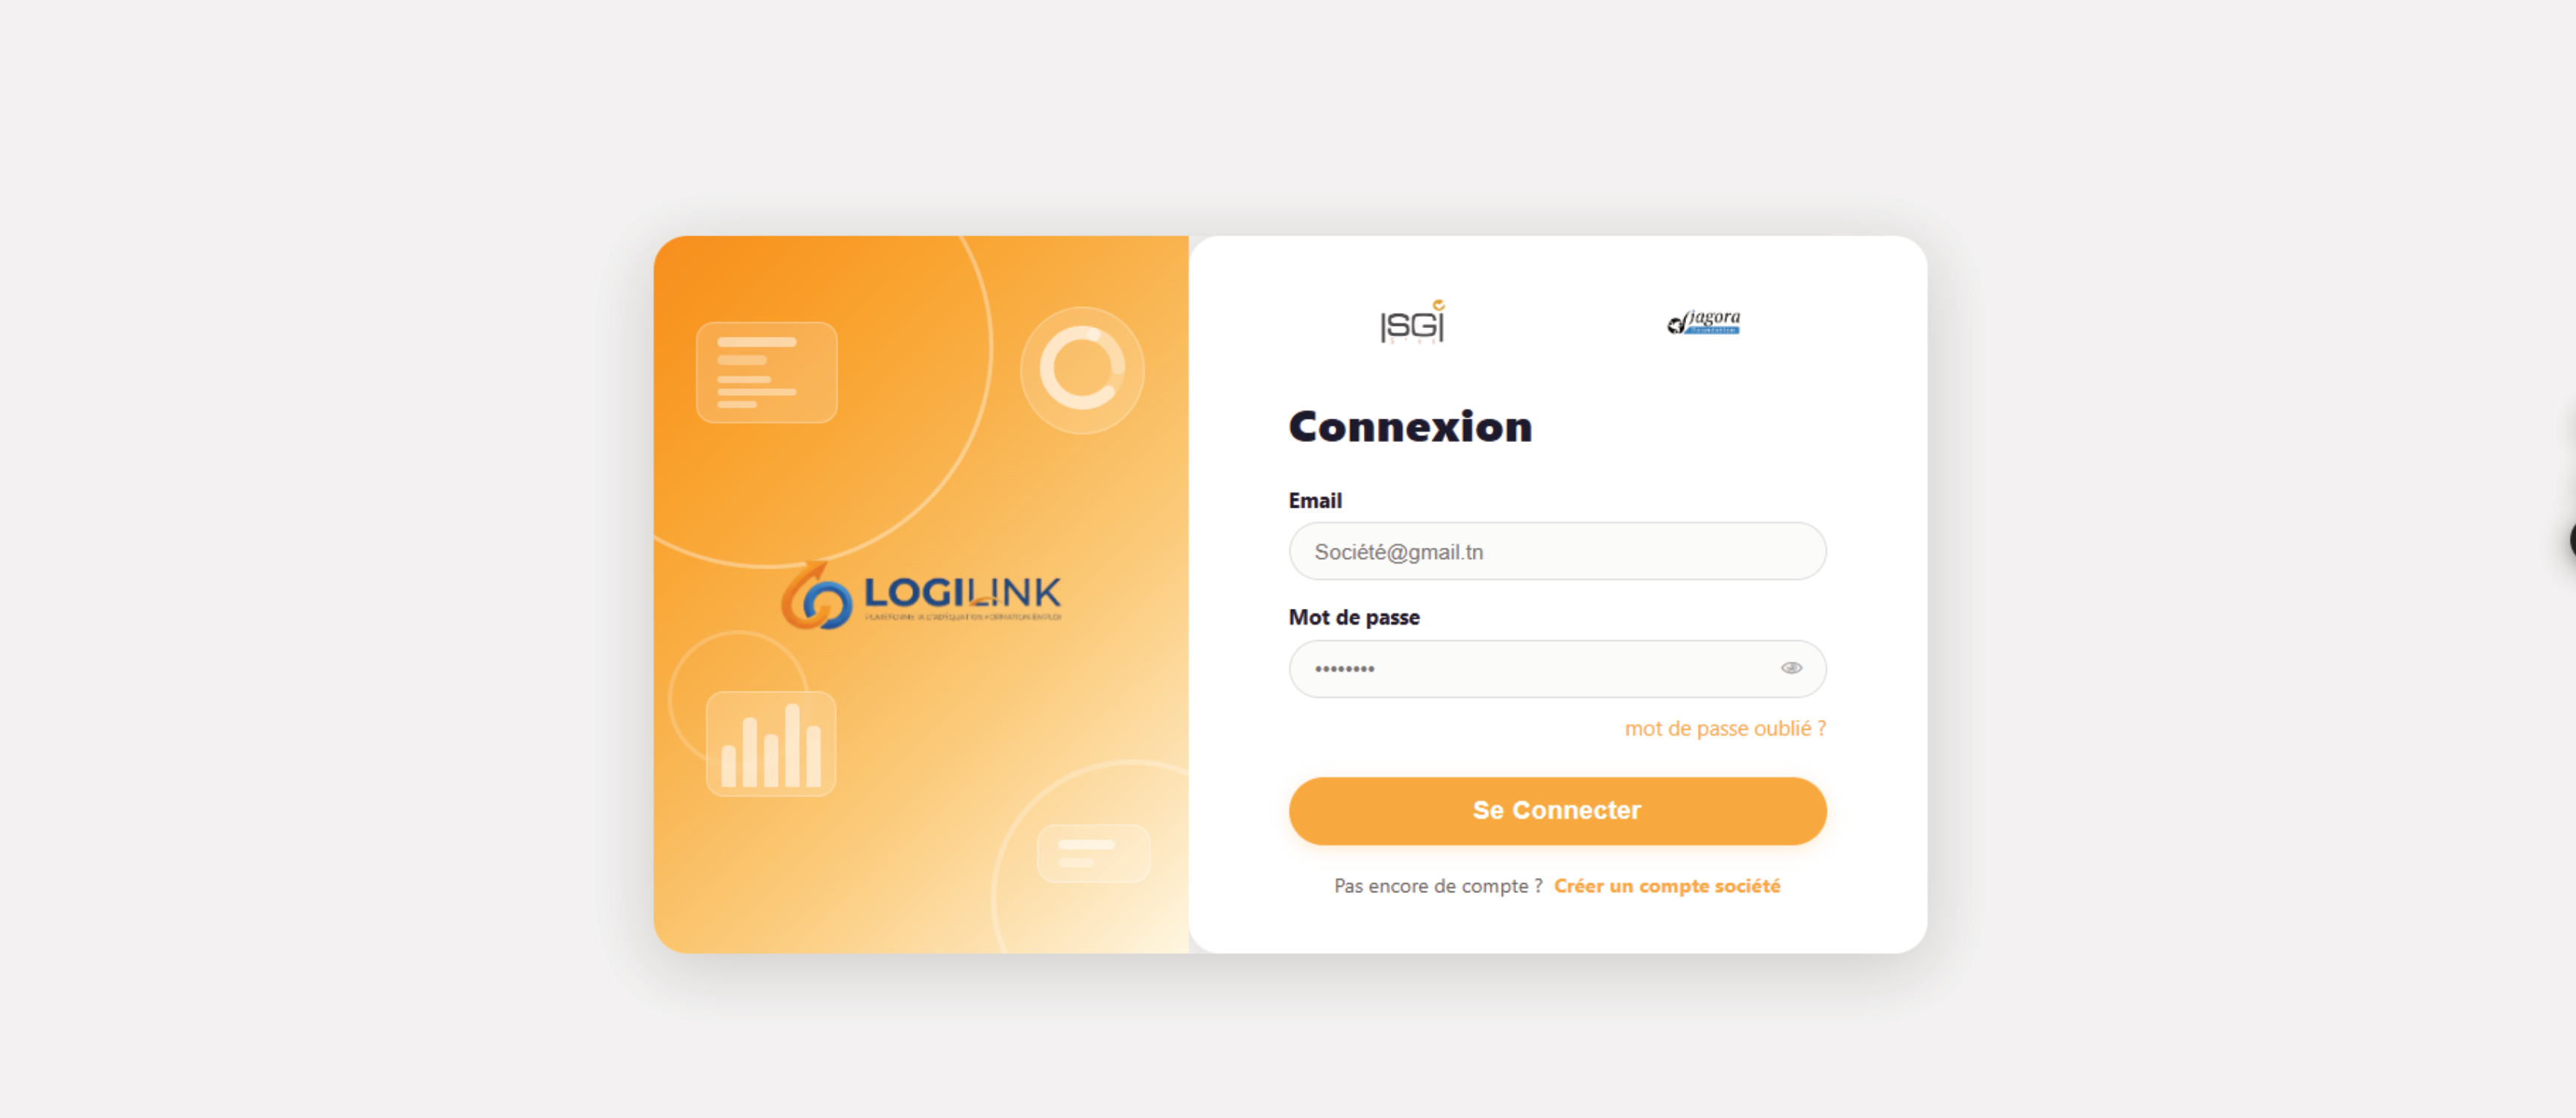
\includegraphics[width=0.85\textwidth]{figures/Interface_daauthentification_des_societes.png}
\caption{Interface d'authentification des sociétés}
\label{fig:authentification-societe}
\end{figure}

\subsection{Interfaces étudiant}

\subsubsection{Profil étudiant}

\noindent La figure~\ref{fig:profil-etudiant} ci-dessous affiche les informations personnelles de l'étudiant.

\begin{figure}[H]
\centering
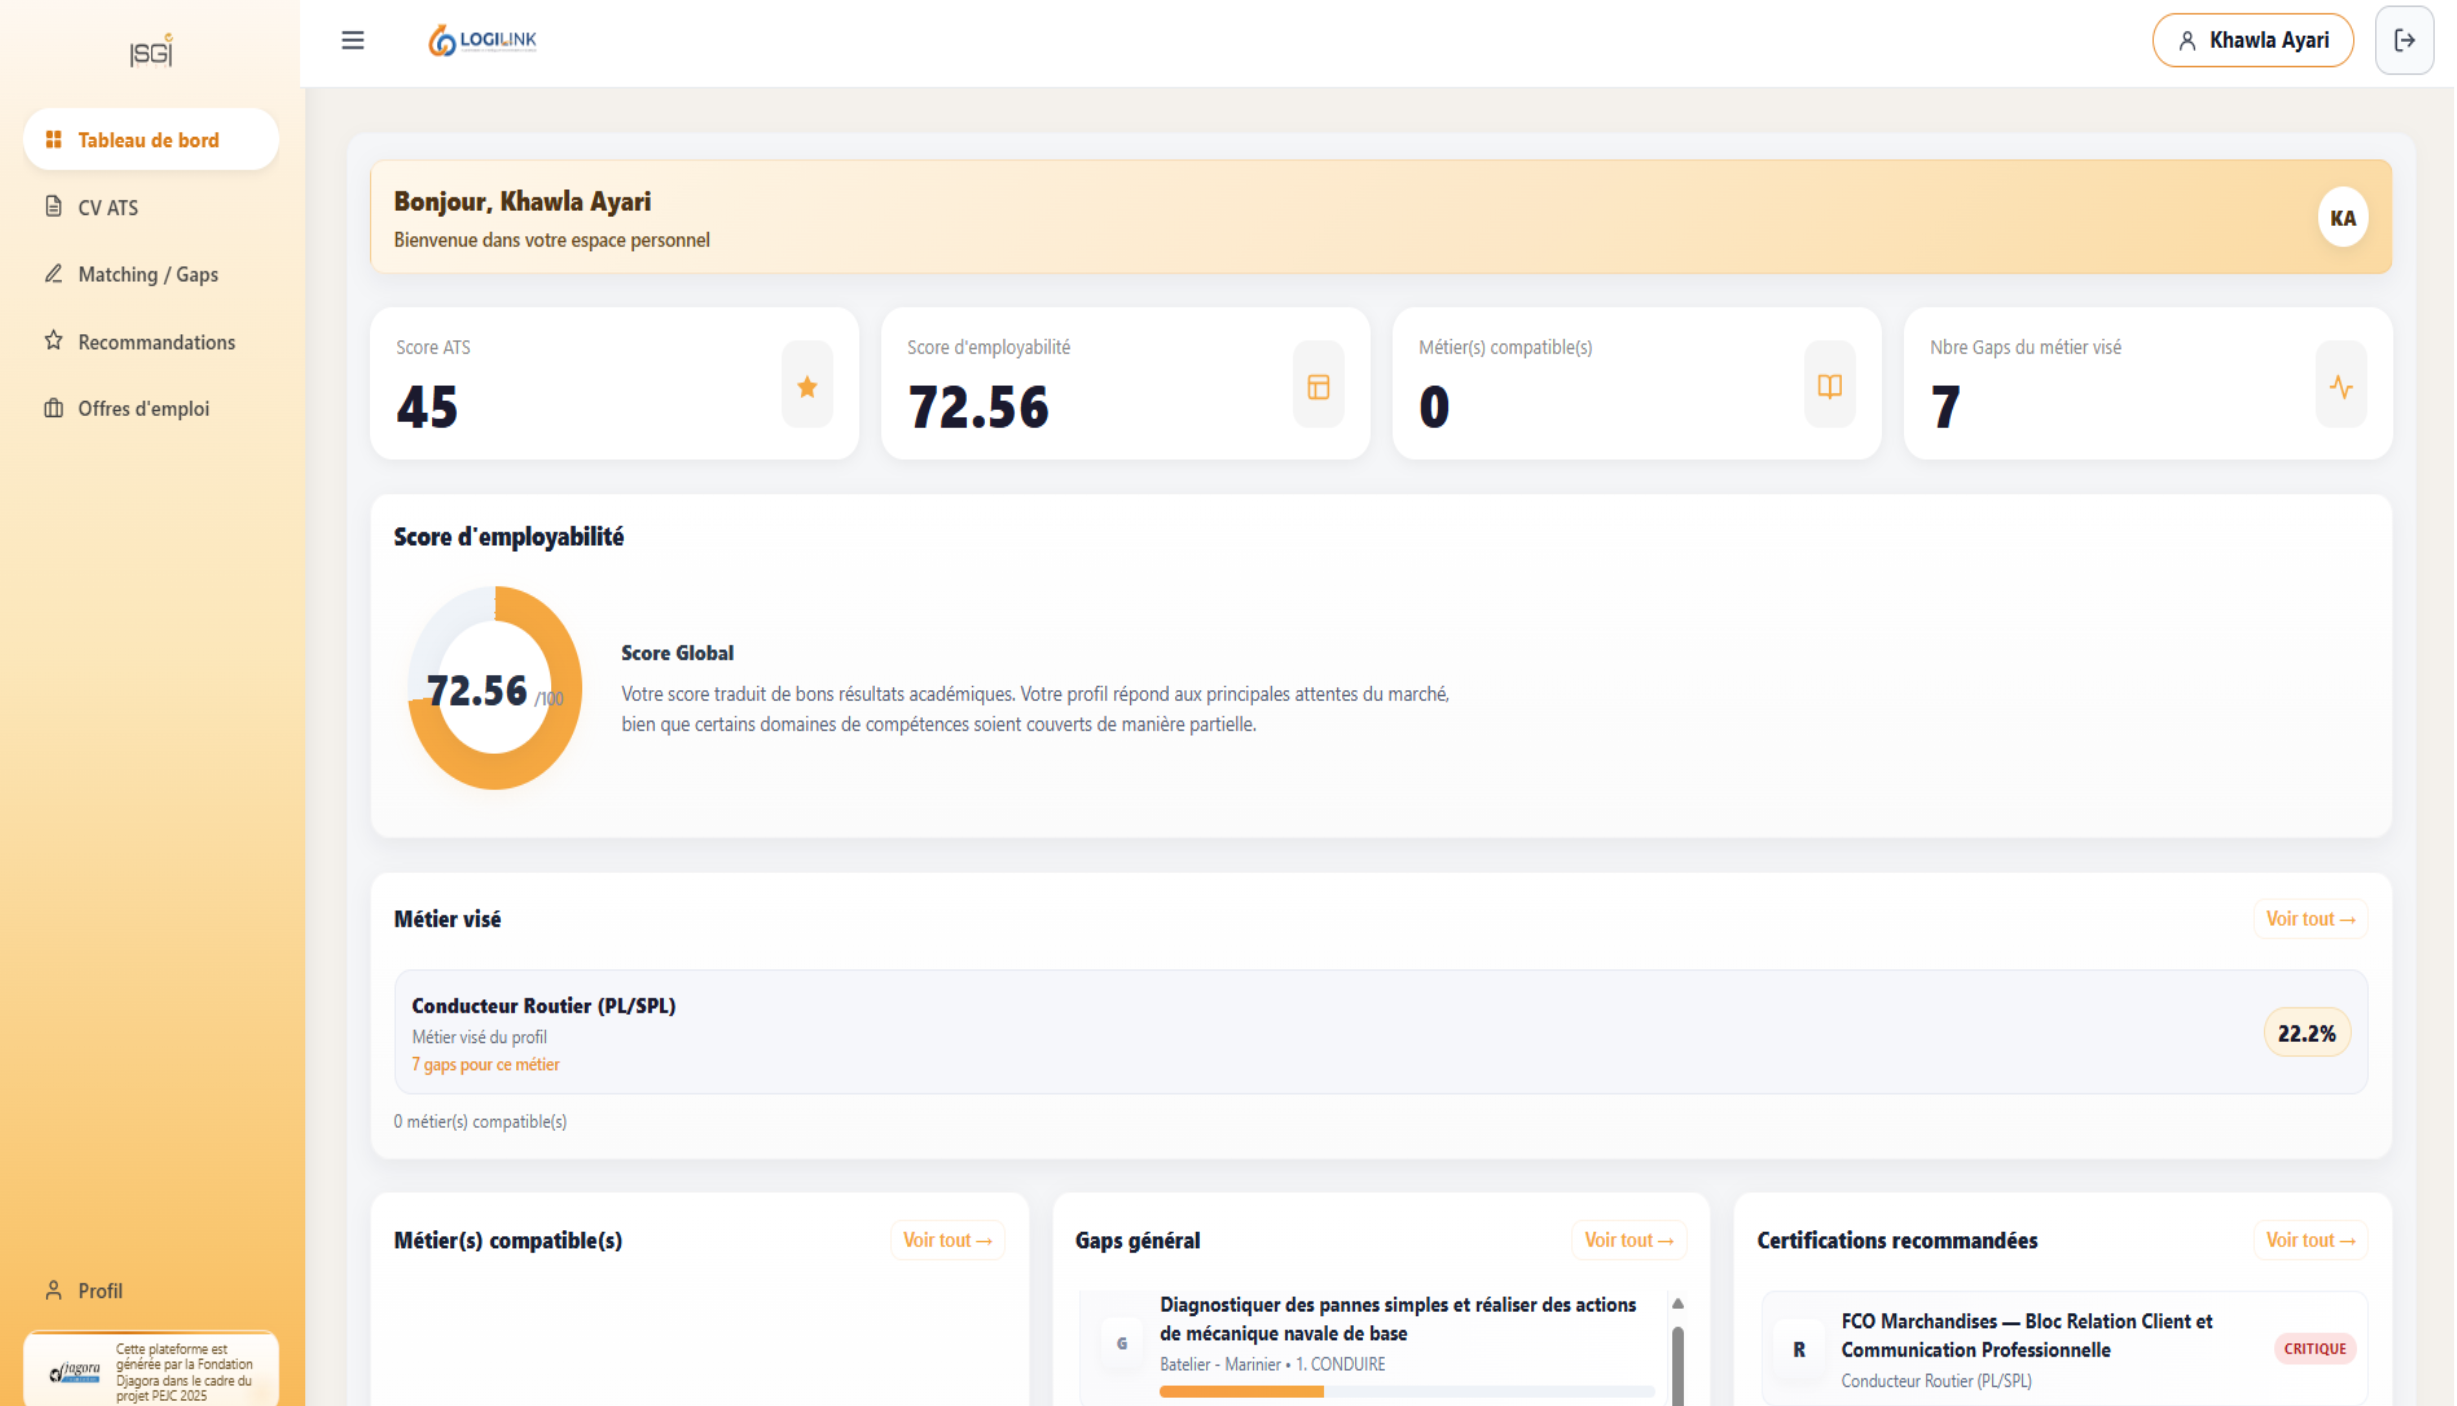
\includegraphics[width=0.85\textwidth]{figures/Interface_du_profil_etudiant.png}
\caption{Interface du profil étudiant}
\label{fig:profil-etudiant}
\end{figure}

\subsubsection{Génération du CV ATS}

La figure~\ref{fig:generation-cv-ats} ci-dessous illustre l'interface de génération du CV ATS, structurée en 11 étapes successives pour garantir un parcours utilisateur fluide. Pour optimiser la saisie, le système intègre un mécanisme d'importation automatique des données institutionnelles de l'ISGIS, pré-remplissant les informations personnelles et extrayant les Hard Skills directement depuis le relevé de notes en fonction du poste visé.
Les autres sections (profil, diplômes, stages, soft skills, langues, projets, certifications et activités para-universitaires) sont complétées manuellement.
De plus, un dispositif de restauration des données permet à l'utilisateur, lors de ses connexions ultérieures, de retrouver et de modifier instantanément ses informations.

\begin{figure}[H]
\centering
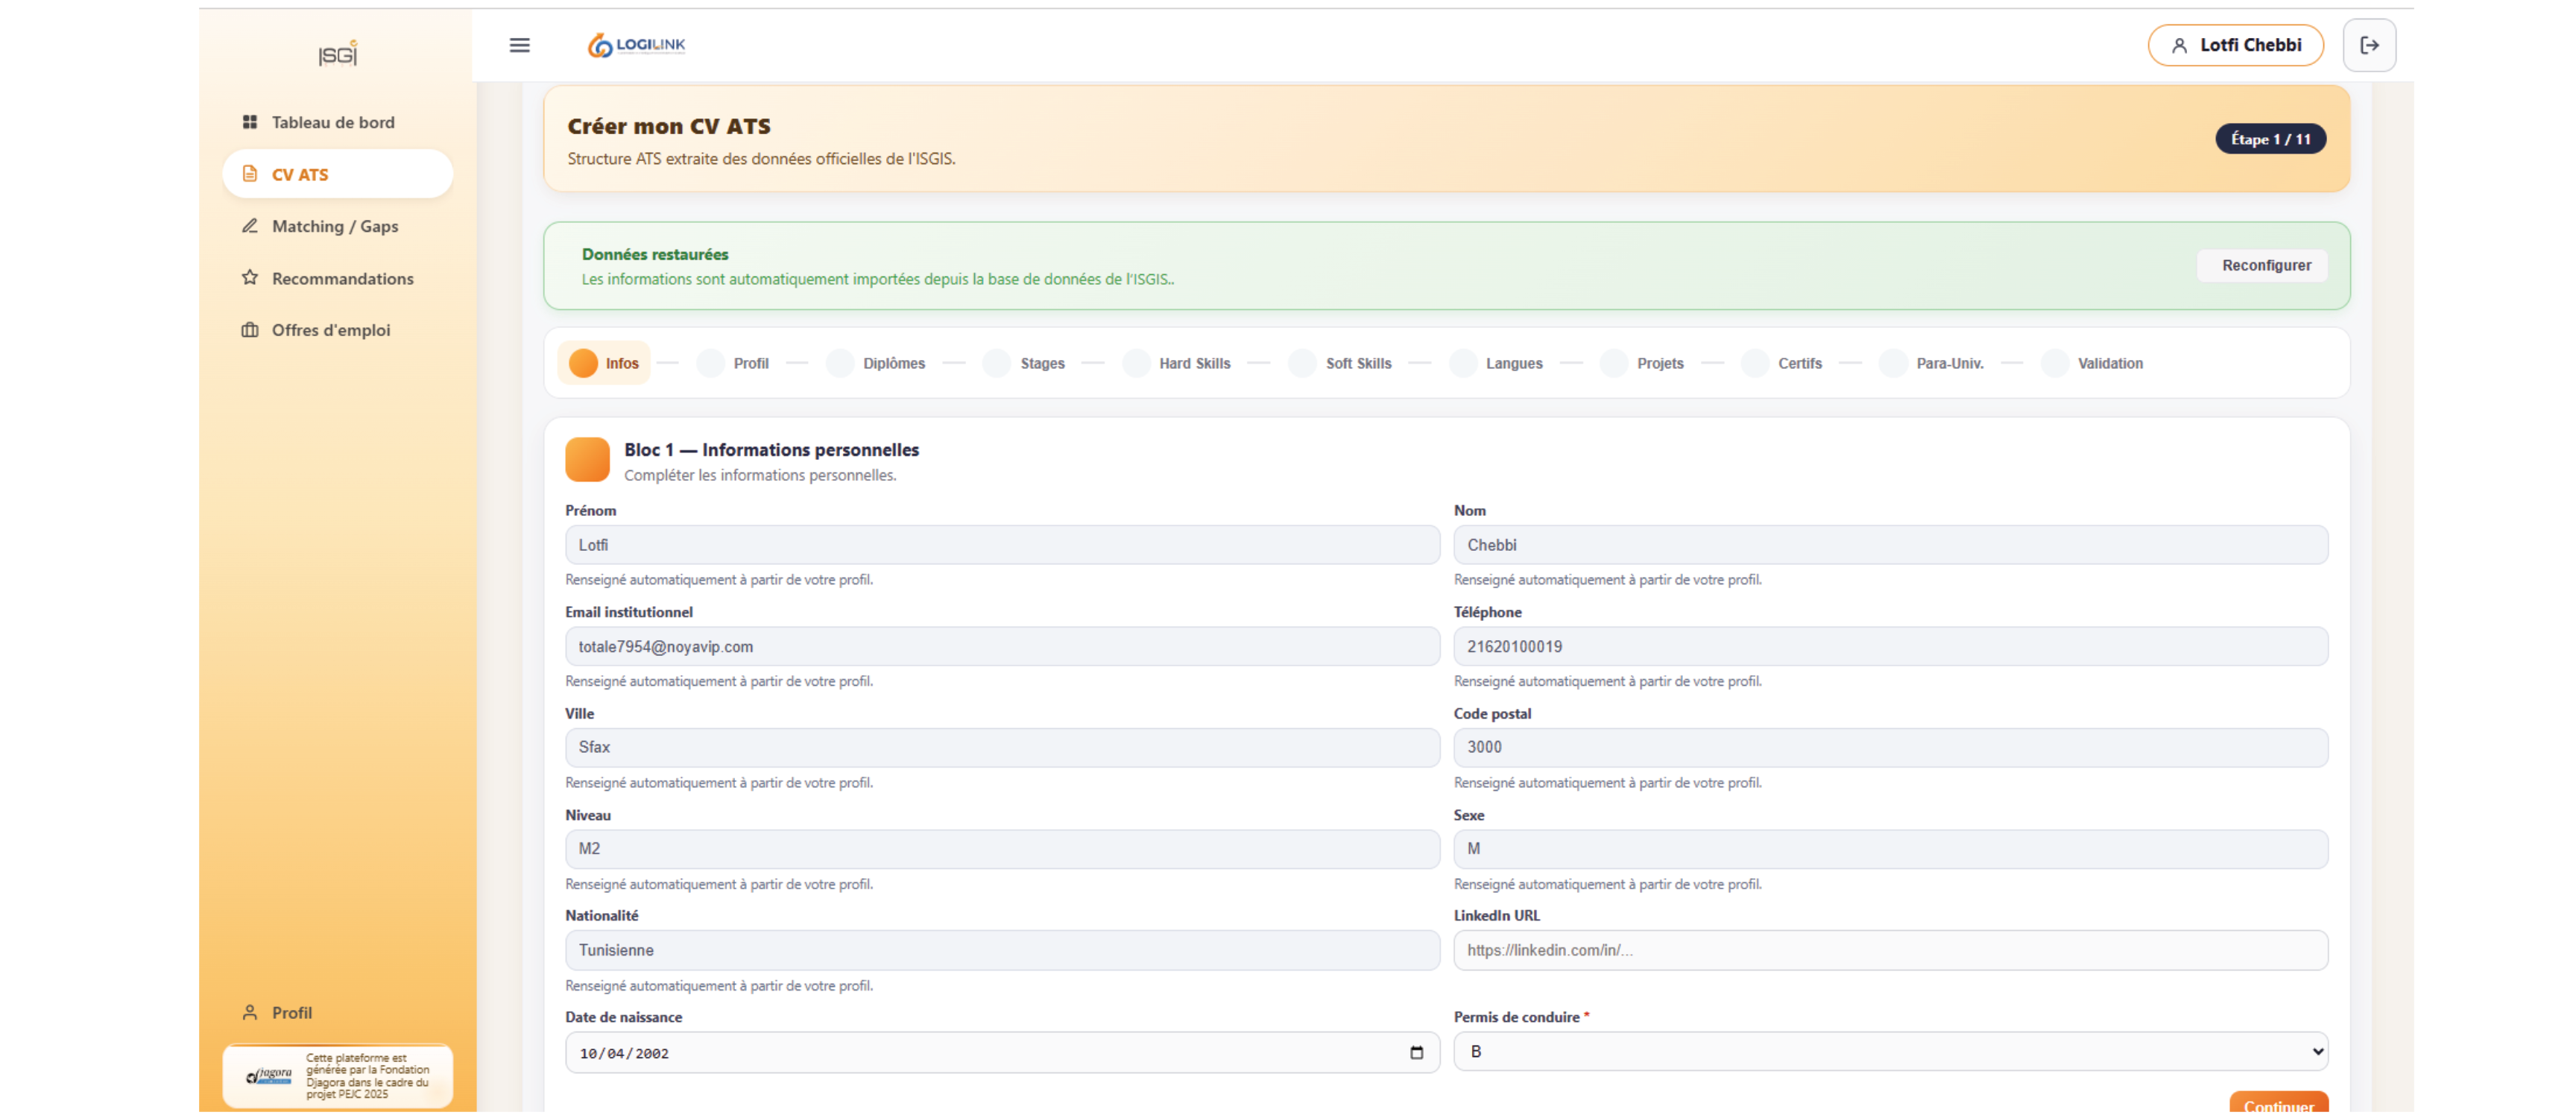
\includegraphics[width=0.85\textwidth]{figures/Interface_de_generation_du_CV_ATS.png}
\caption{Interface de génération du CV ATS}
\label{fig:generation-cv-ats}
\end{figure}

\noindent La figure \ref{fig:validation-cv-ats} présente l'étape finale de validation, qui permet à l'étudiant de vérifier l'ensemble de ses données avant de générer son CV ATS.

\begin{figure}[H]
\centering
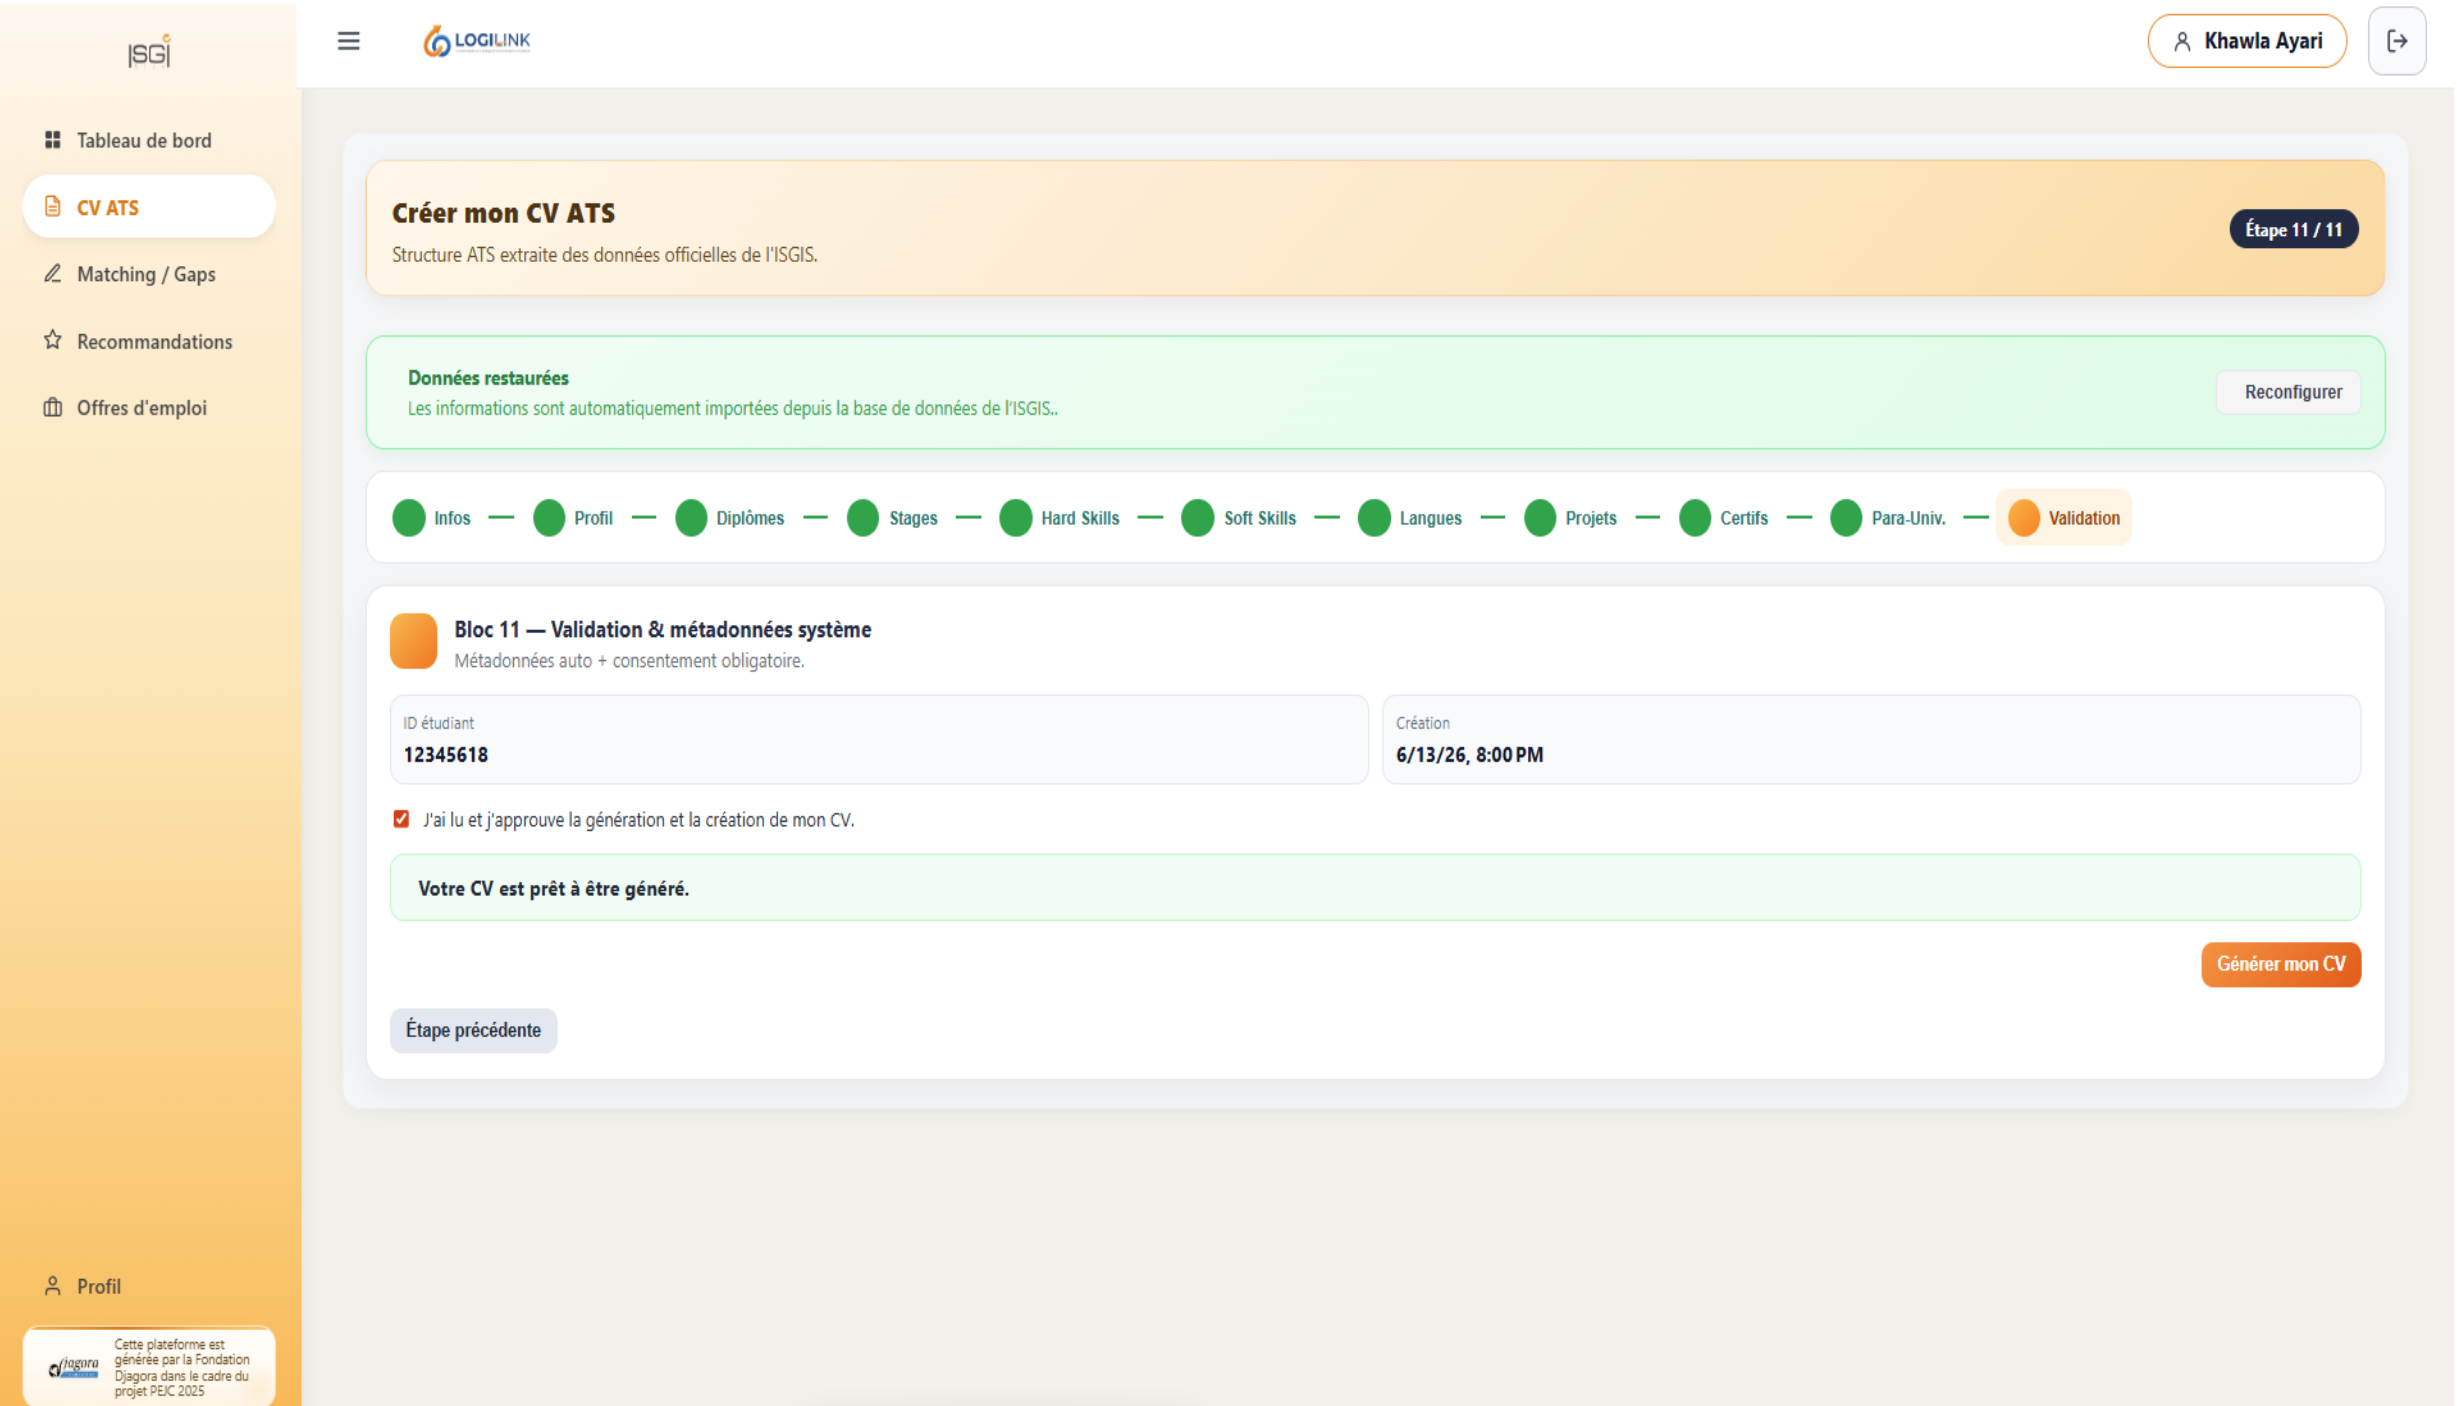
\includegraphics[width=0.85\textwidth]{figures/Interface_de_validation_du_CV_ATS.png}
\caption{Interface de validation du CV ATS}
\label{fig:validation-cv-ats}
\end{figure}

\noindent La figure \ref{fig:cv-ats-genere} illustre le CV généré. Depuis cet espace, l'étudiant a la possibilité de modifier ses informations, de télécharger son document au format PDF et de cliquer sur le bouton "Évaluer votre CV" afin de stocker le CV, lancer le calcul de ses scores ATS et d'employabilité.

\begin{figure}[H]
\centering
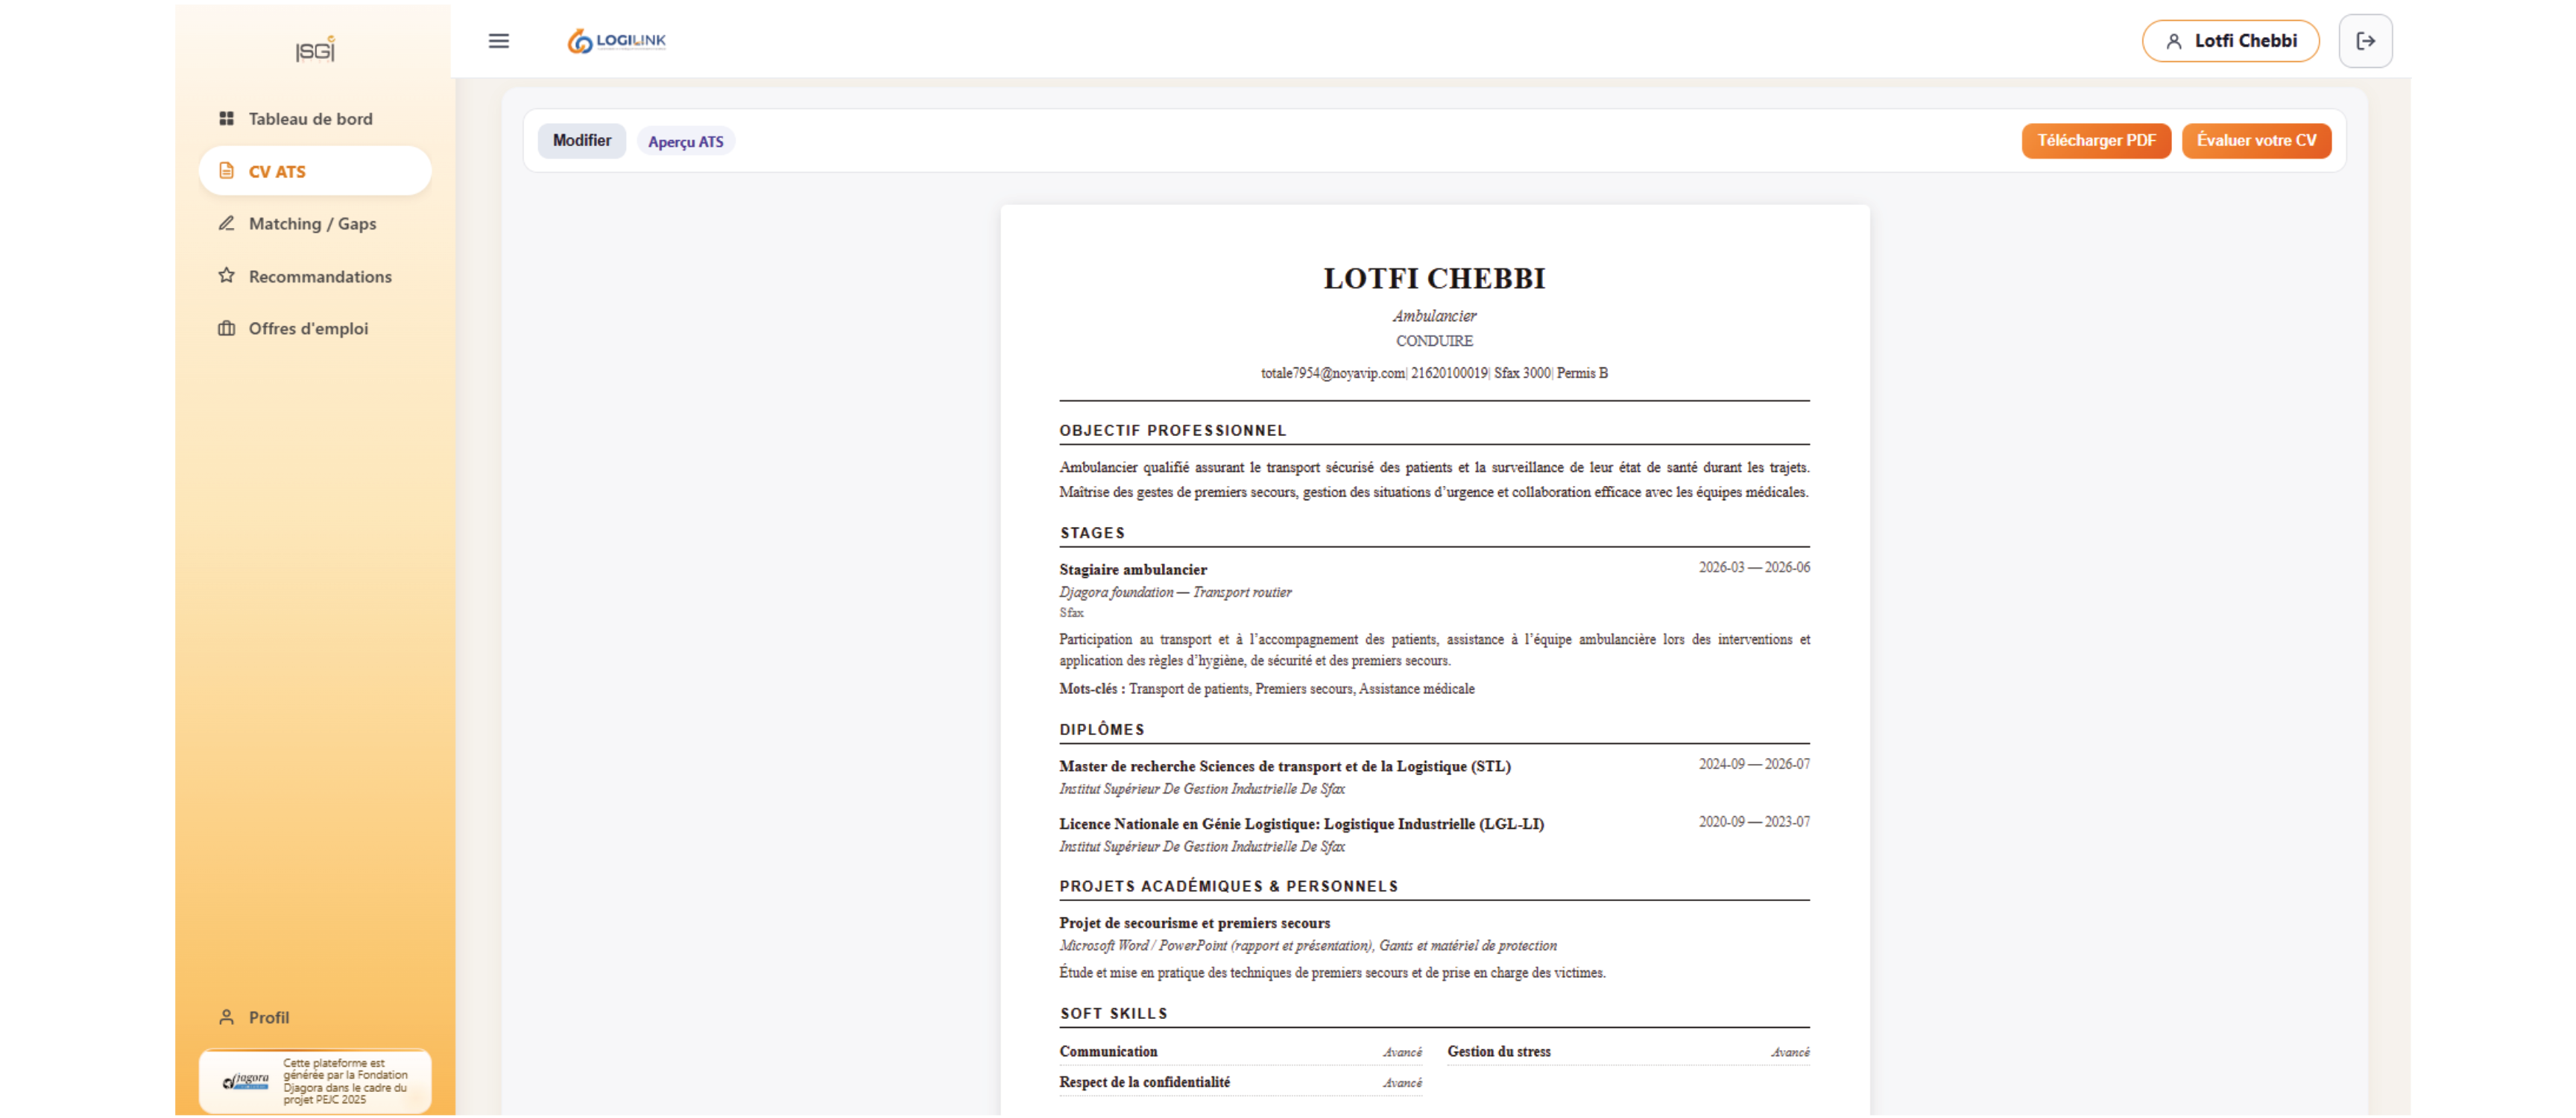
\includegraphics[width=0.85\textwidth]{figures/Interface_du_CV_ATS_genere.png}
\caption{Interface du CV ATS généré}
\label{fig:cv-ats-genere}
\end{figure}

\subsubsection{Calcul du score ats et employabilité}

La figure \ref{fig:tableau-bord-etudiant} ci-dessous présente le tableau de bord principal de l'étudiant. Cet espace regroupe les résultats d'analyse de la plateforme et affiche les scores ATS et d'employabilité.

\begin{figure}[H]
\centering
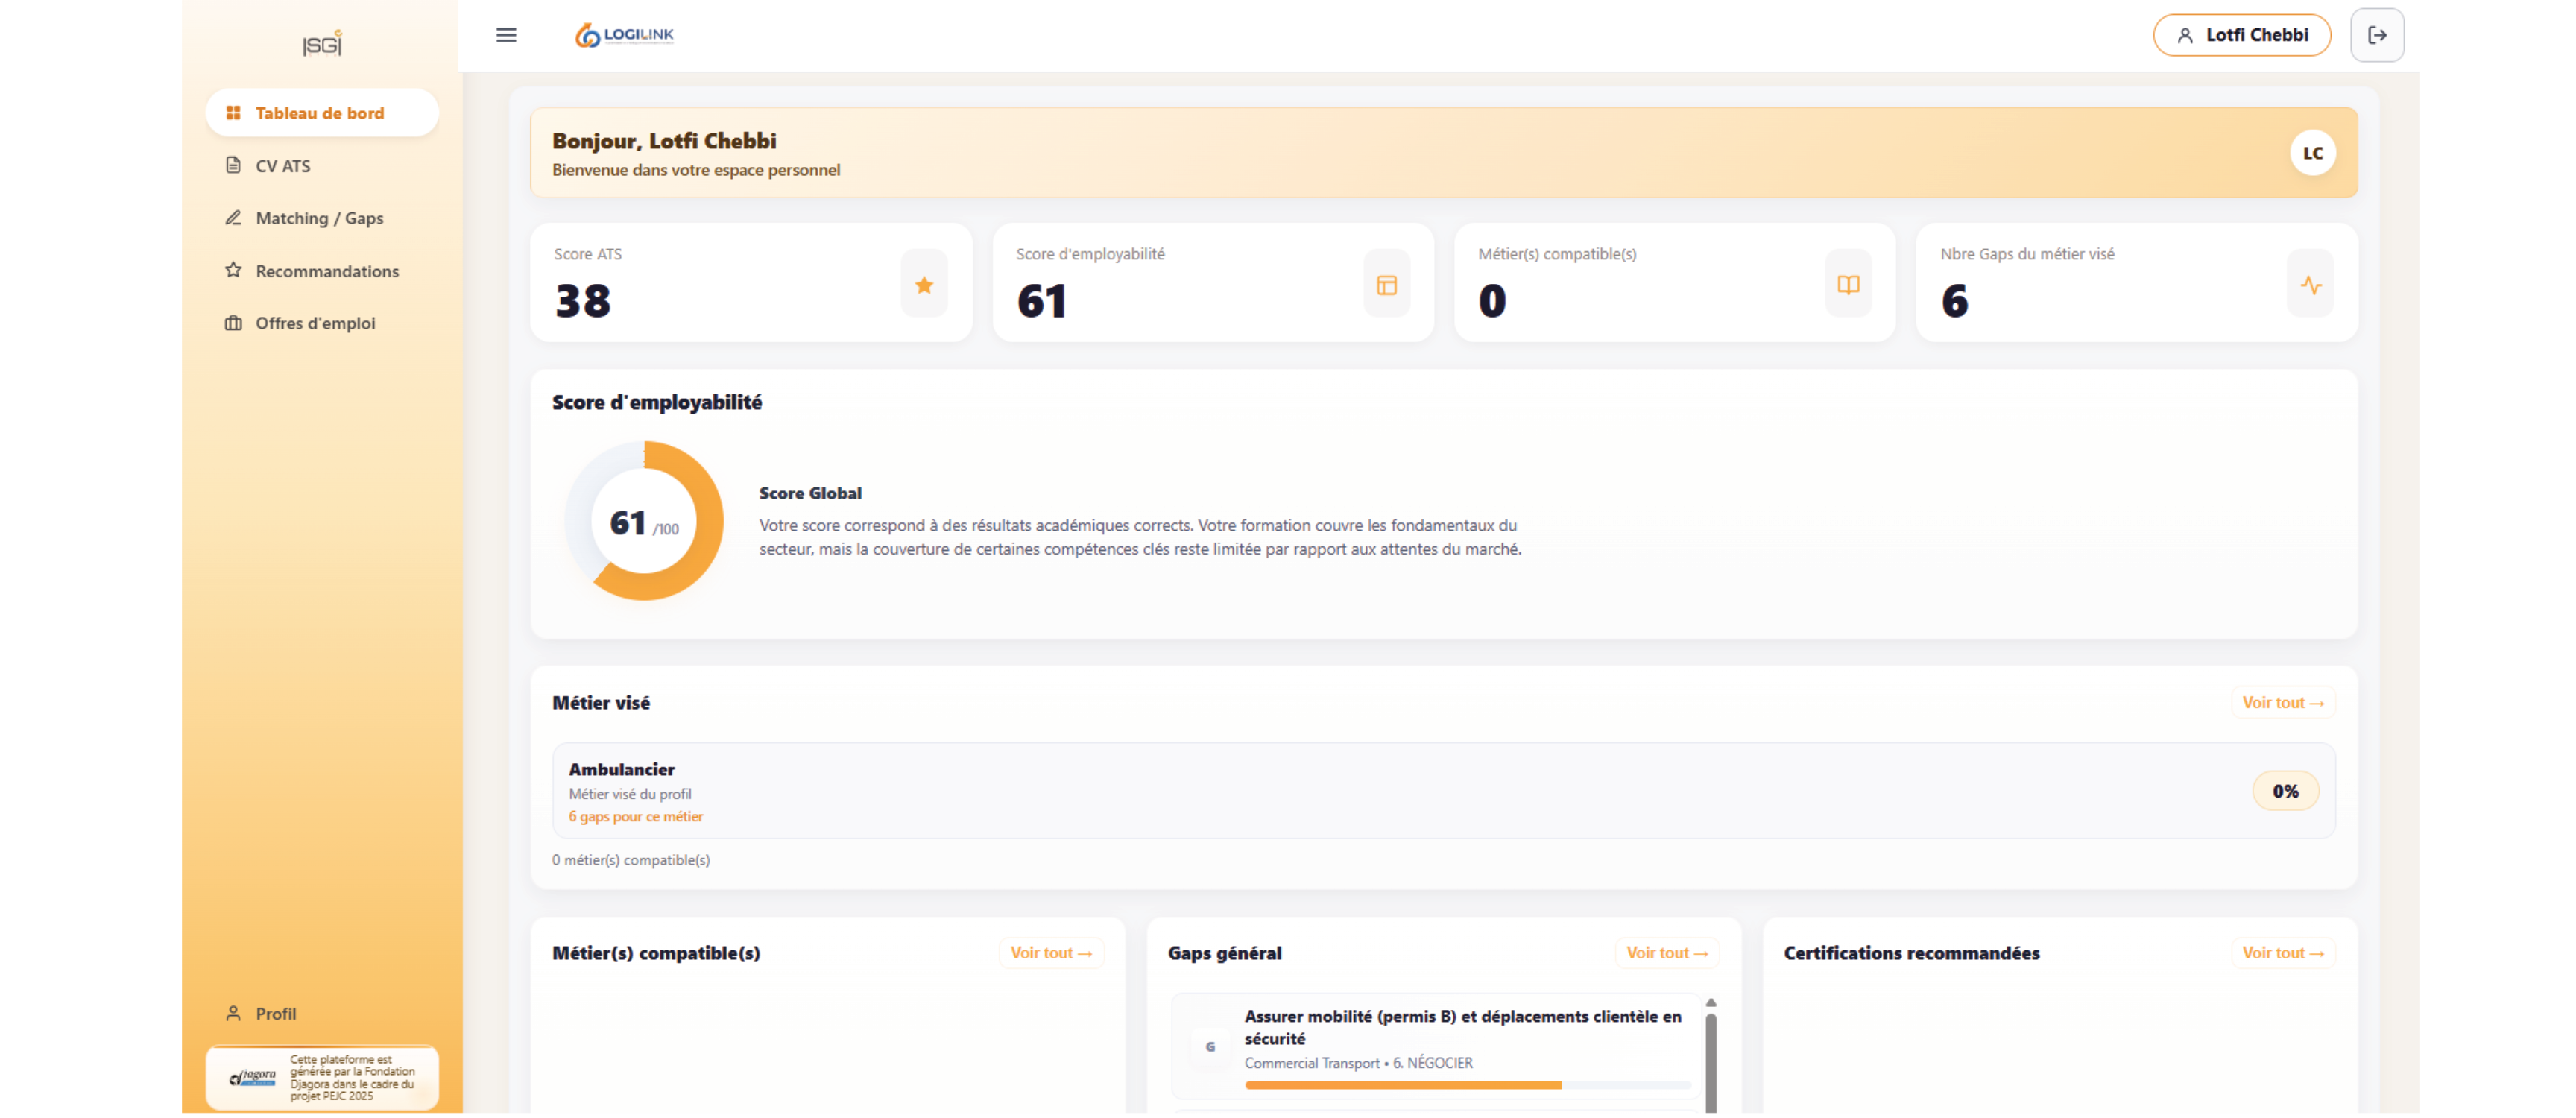
\includegraphics[width=0.85\textwidth]{figures/Interface_du_tableau_de_bord_de_laetudiant.png}
\caption{Interface du tableau de bord de l'étudiant}
\label{fig:tableau-bord-etudiant}
\end{figure}

\subsubsection{Calcul du score d'employabilité prévisionnel}

\noindent La figure~\ref{fig:prediction-score-employabilite} suivante montre que lorsque l'étudiant clique sur le bouton "Prédire votre nouveau score", un score d'employabilité prévisionnel est automatiquement généré en tenant compte des recommandations obtenues.

\begin{figure}[H]
\centering
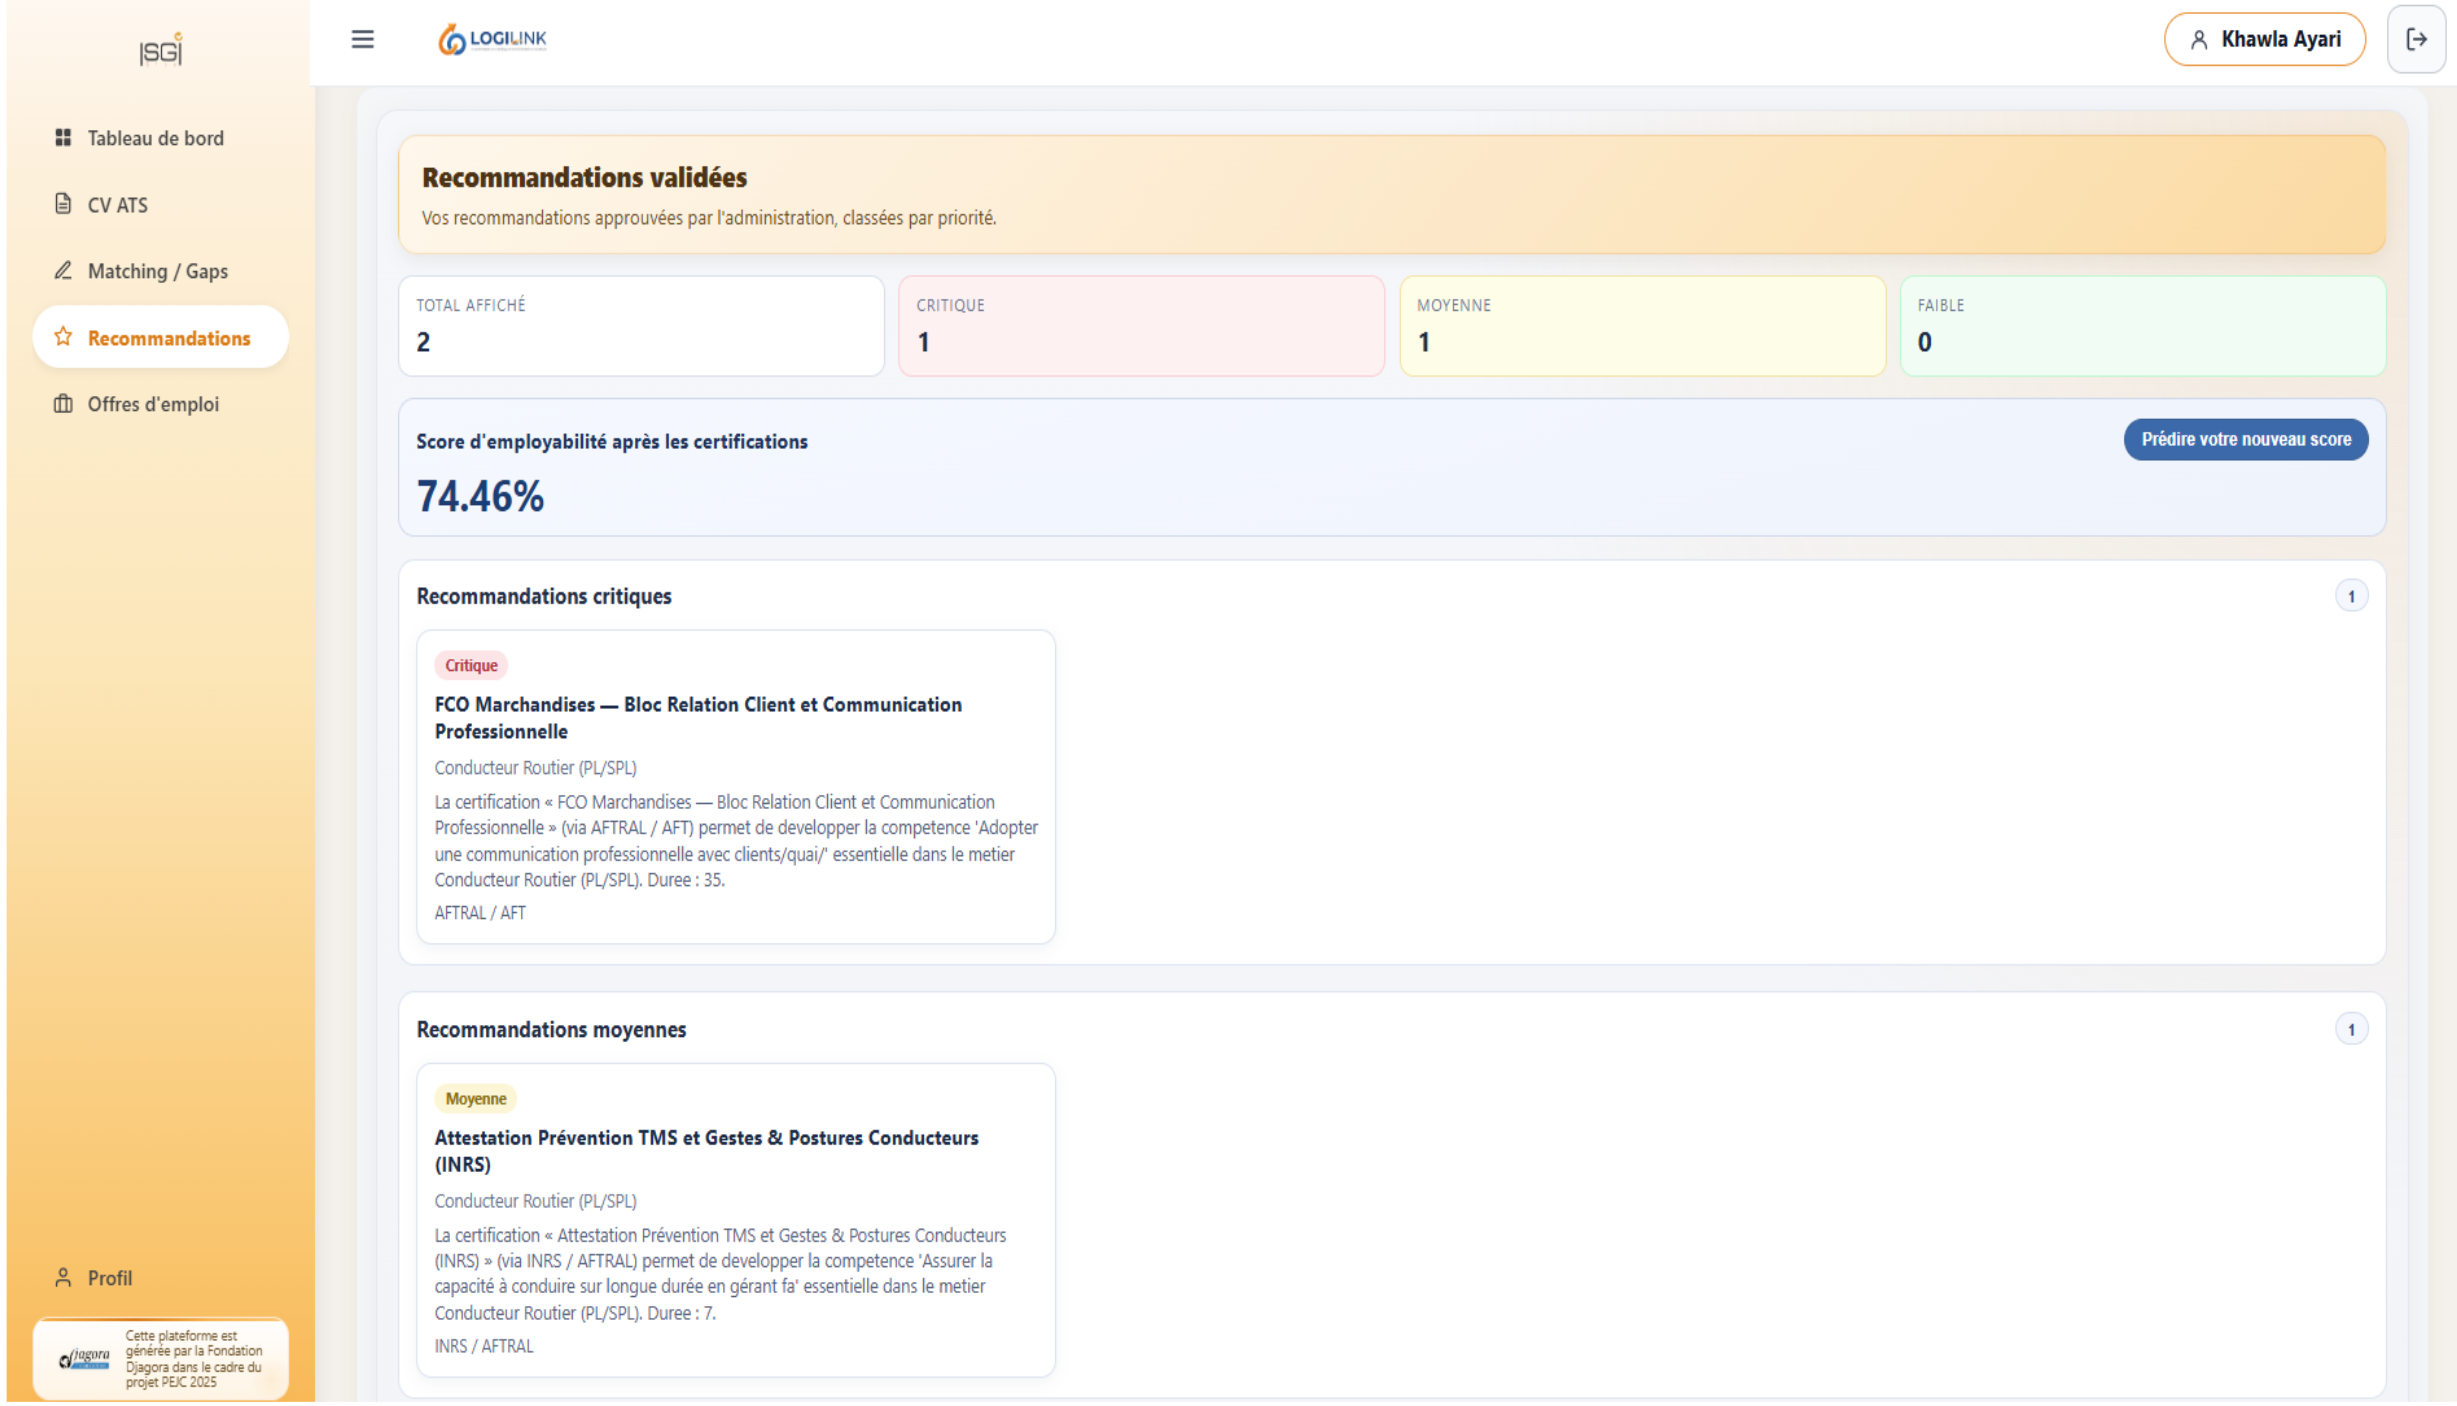
\includegraphics[width=0.85\textwidth]{figures/Interface_de_prediction_du_score_daemployabilite.png}
\caption{Interface de prédiction du score d'employabilité}
\label{fig:prediction-score-employabilite}
\end{figure}

\subsection{Interfaces admin}

\noindent Les figures~\ref{fig:tableau-bord-admin}~et~\ref{fig:tableau-bord-admin-2} ci-dessous présentent le tableau de bord de l'administrateur, un espace de pilotage centralisant les indicateurs clés ainsi que des graphiques d'analyse. Elle permet de visualiser la répartition des étudiants par filière, d'observer la distribution des scores ATS et des scores d'employabilité, et de consulter une liste des étudiants les mieux classés selon le score d'employabilité.

\begin{figure}[H]
\centering
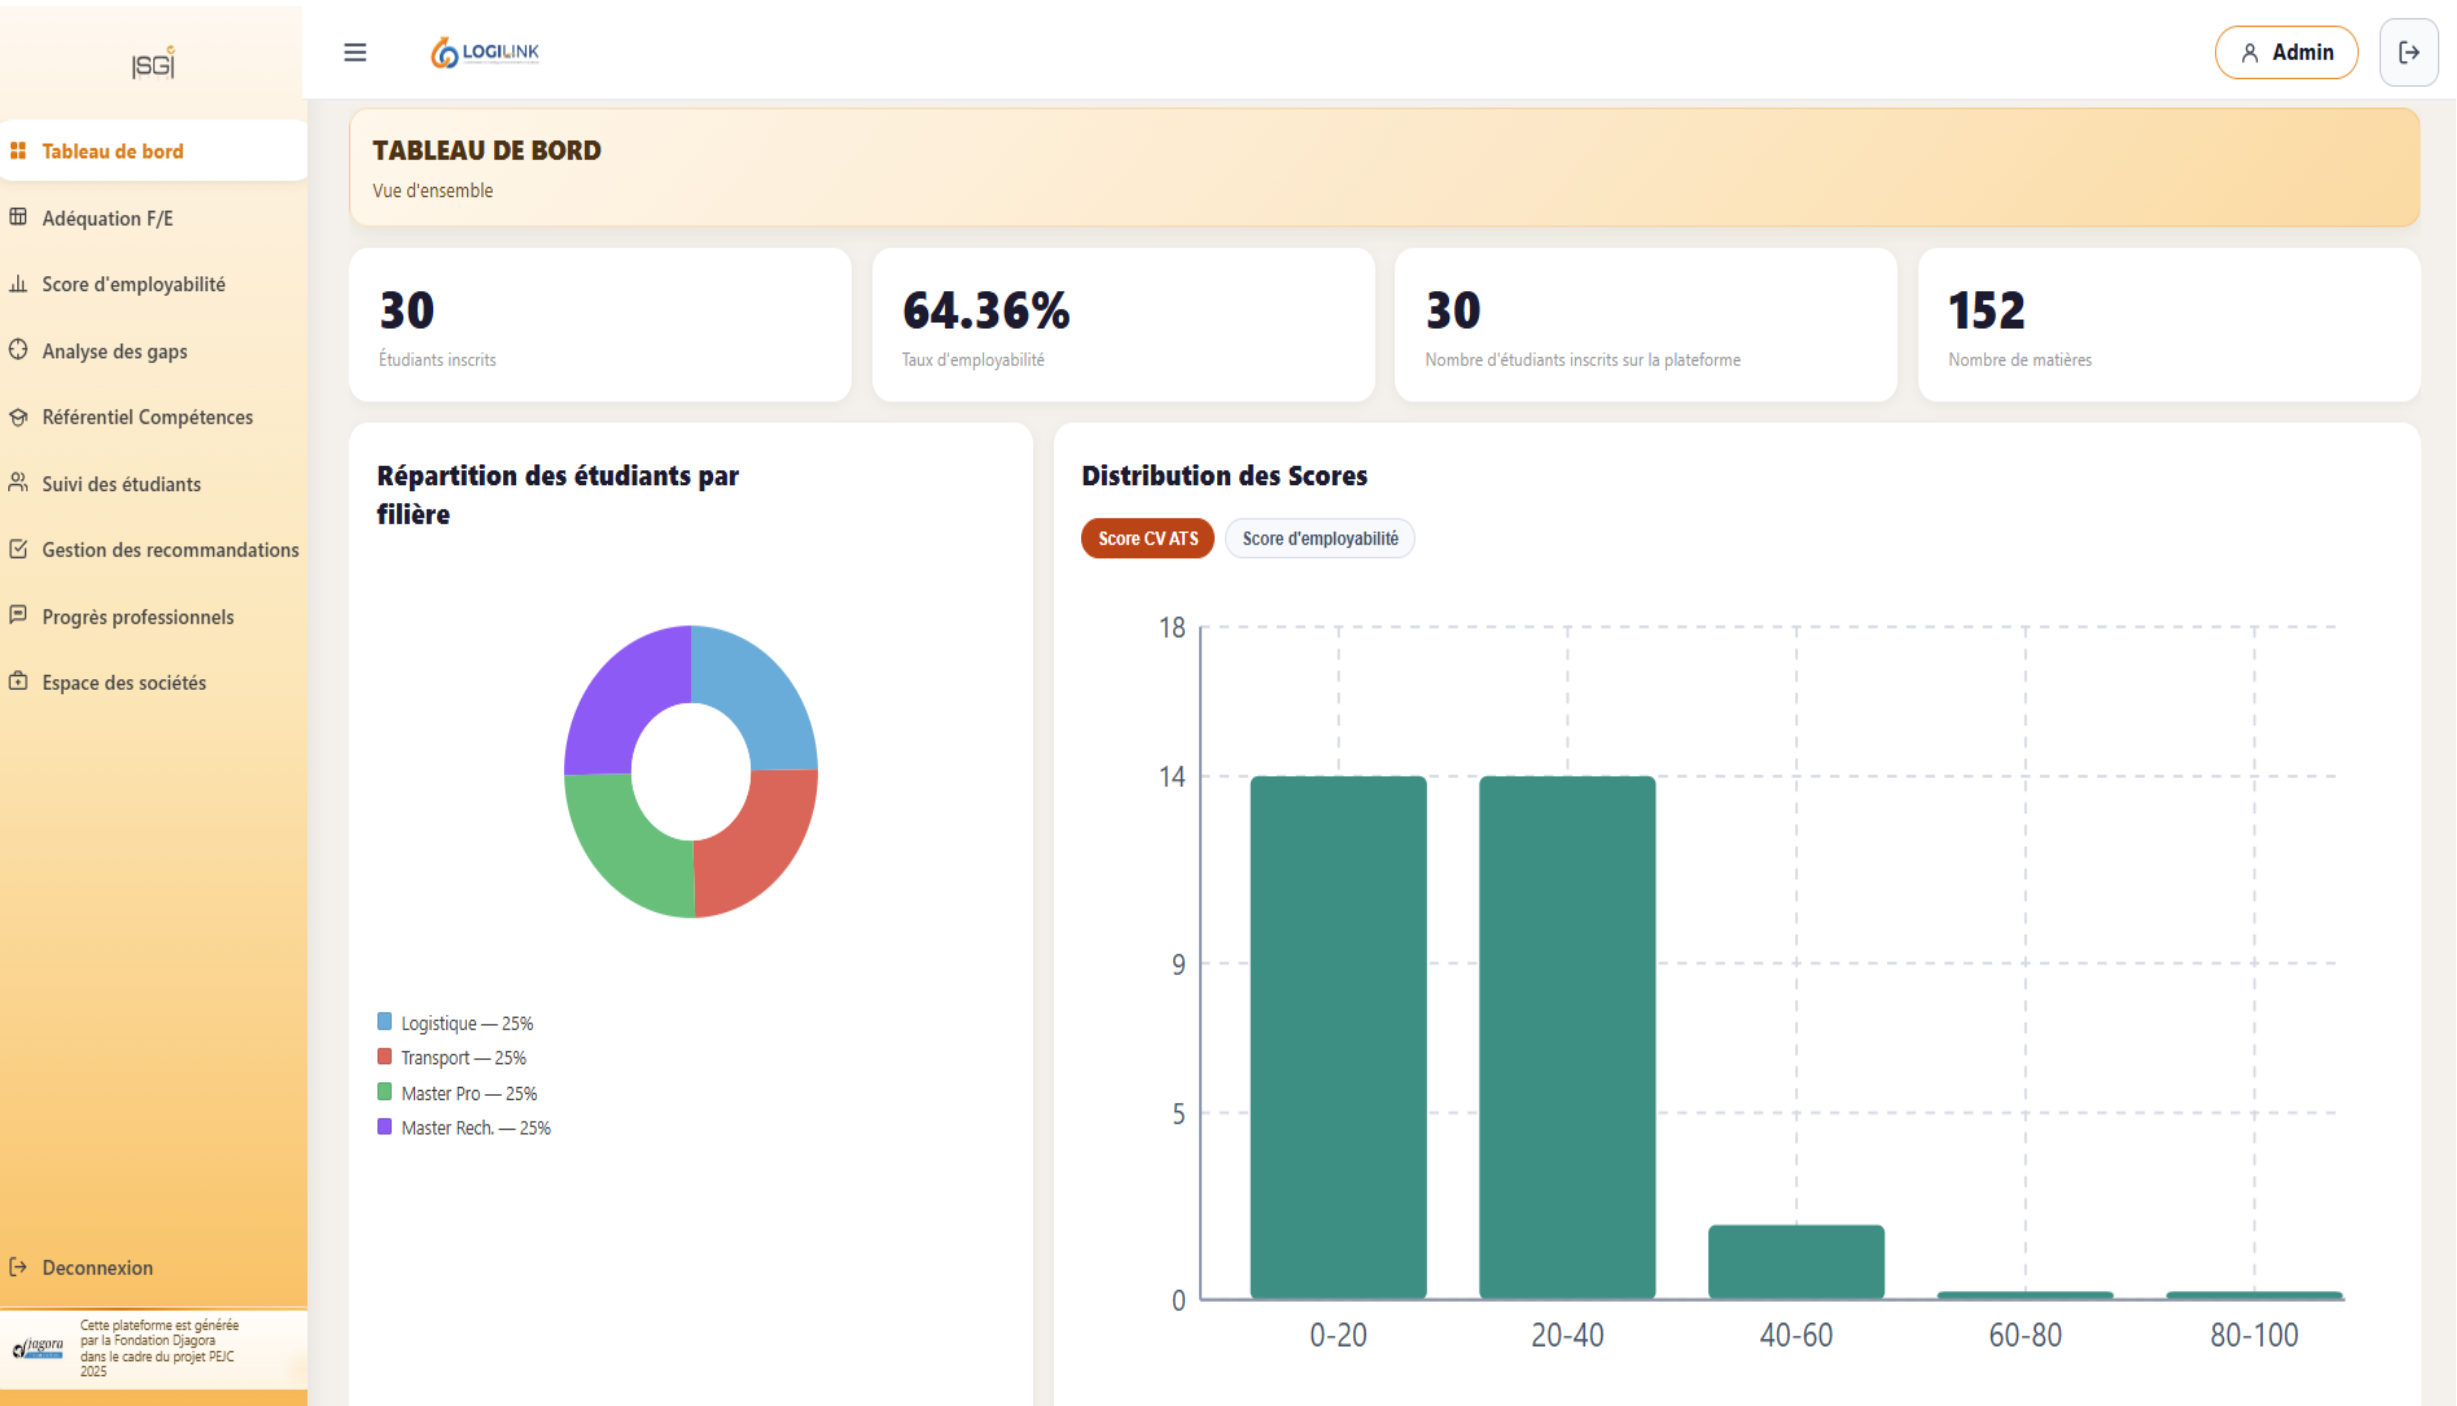
\includegraphics[width=0.85\textwidth]{figures/Interface_du_tableau_de_bord_de_laadministrateur.png}
\caption{Interface du tableau de bord de l'administrateur}
\label{fig:tableau-bord-admin}
\end{figure}

\begin{figure}[H]
\centering
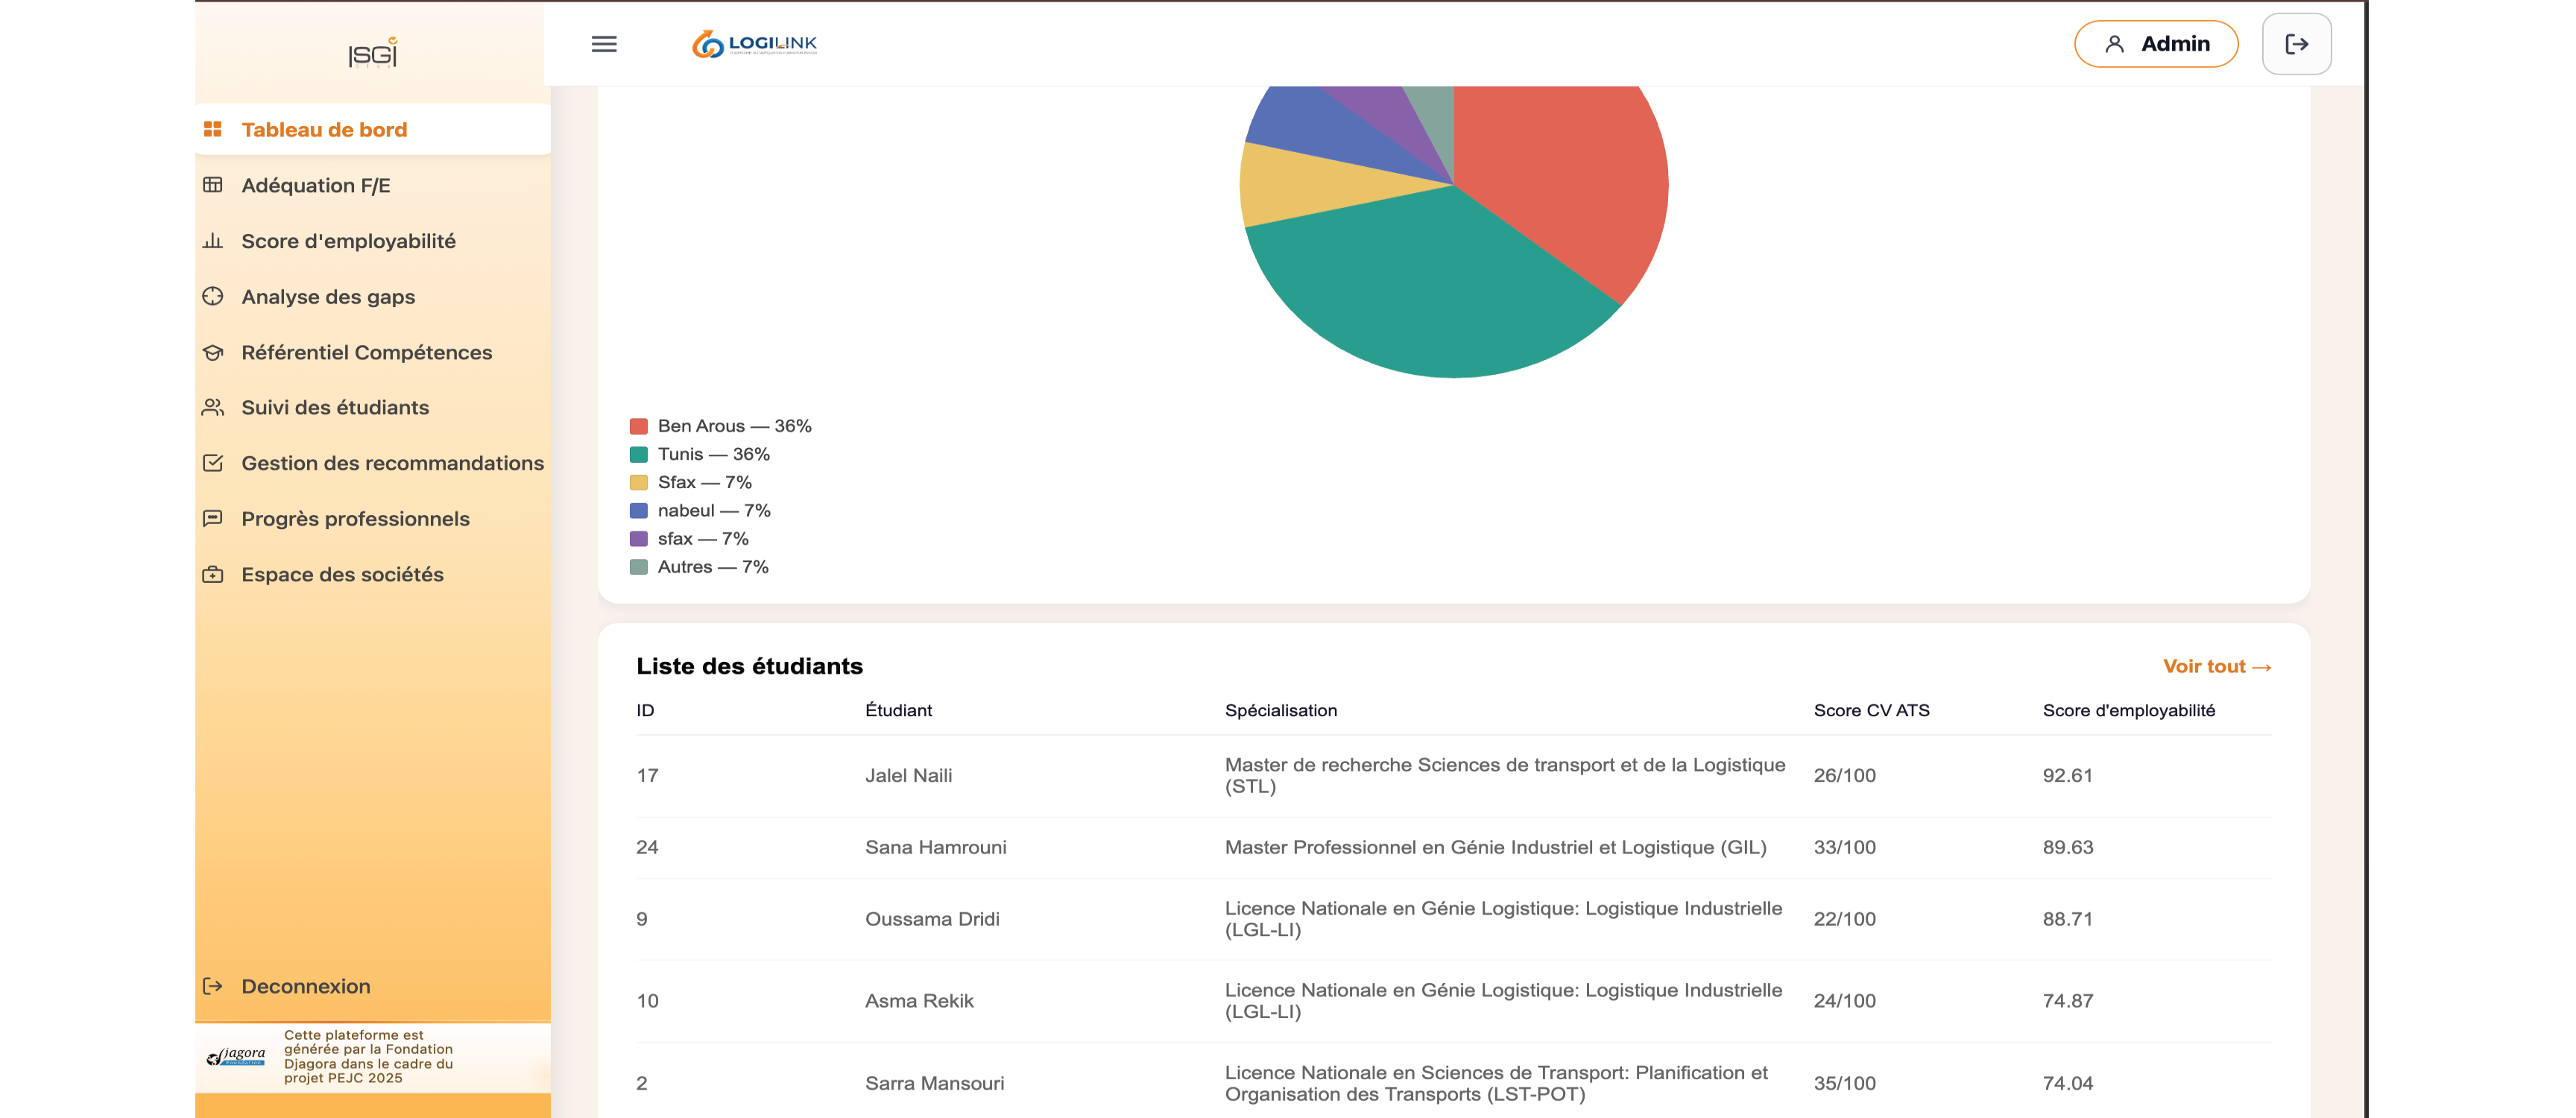
\includegraphics[width=0.85\textwidth]{figures/Interface_du_tableau_de_bord_de_laadministrateur_2.png}
\caption{Interface du tableau de bord de l'administrateur}
\label{fig:tableau-bord-admin-2}
\end{figure}

\noindent Les figures~\ref{fig:score-employabilite}~et~\ref{fig:score-employabilite-2} ci-dessous illustrent l'interface Score d'employabilité. Elle présente le nombre d'étudiants inscrits, le nombre d'étudiants classés parmi les meilleurs profils, ainsi que le score global d'employabilité. L'interface propose ensuite la distribution des scores, une analyse par filière et une comparaison par type de parcours (Licence, Master, Licence + Master).

\begin{figure}[H]
\centering
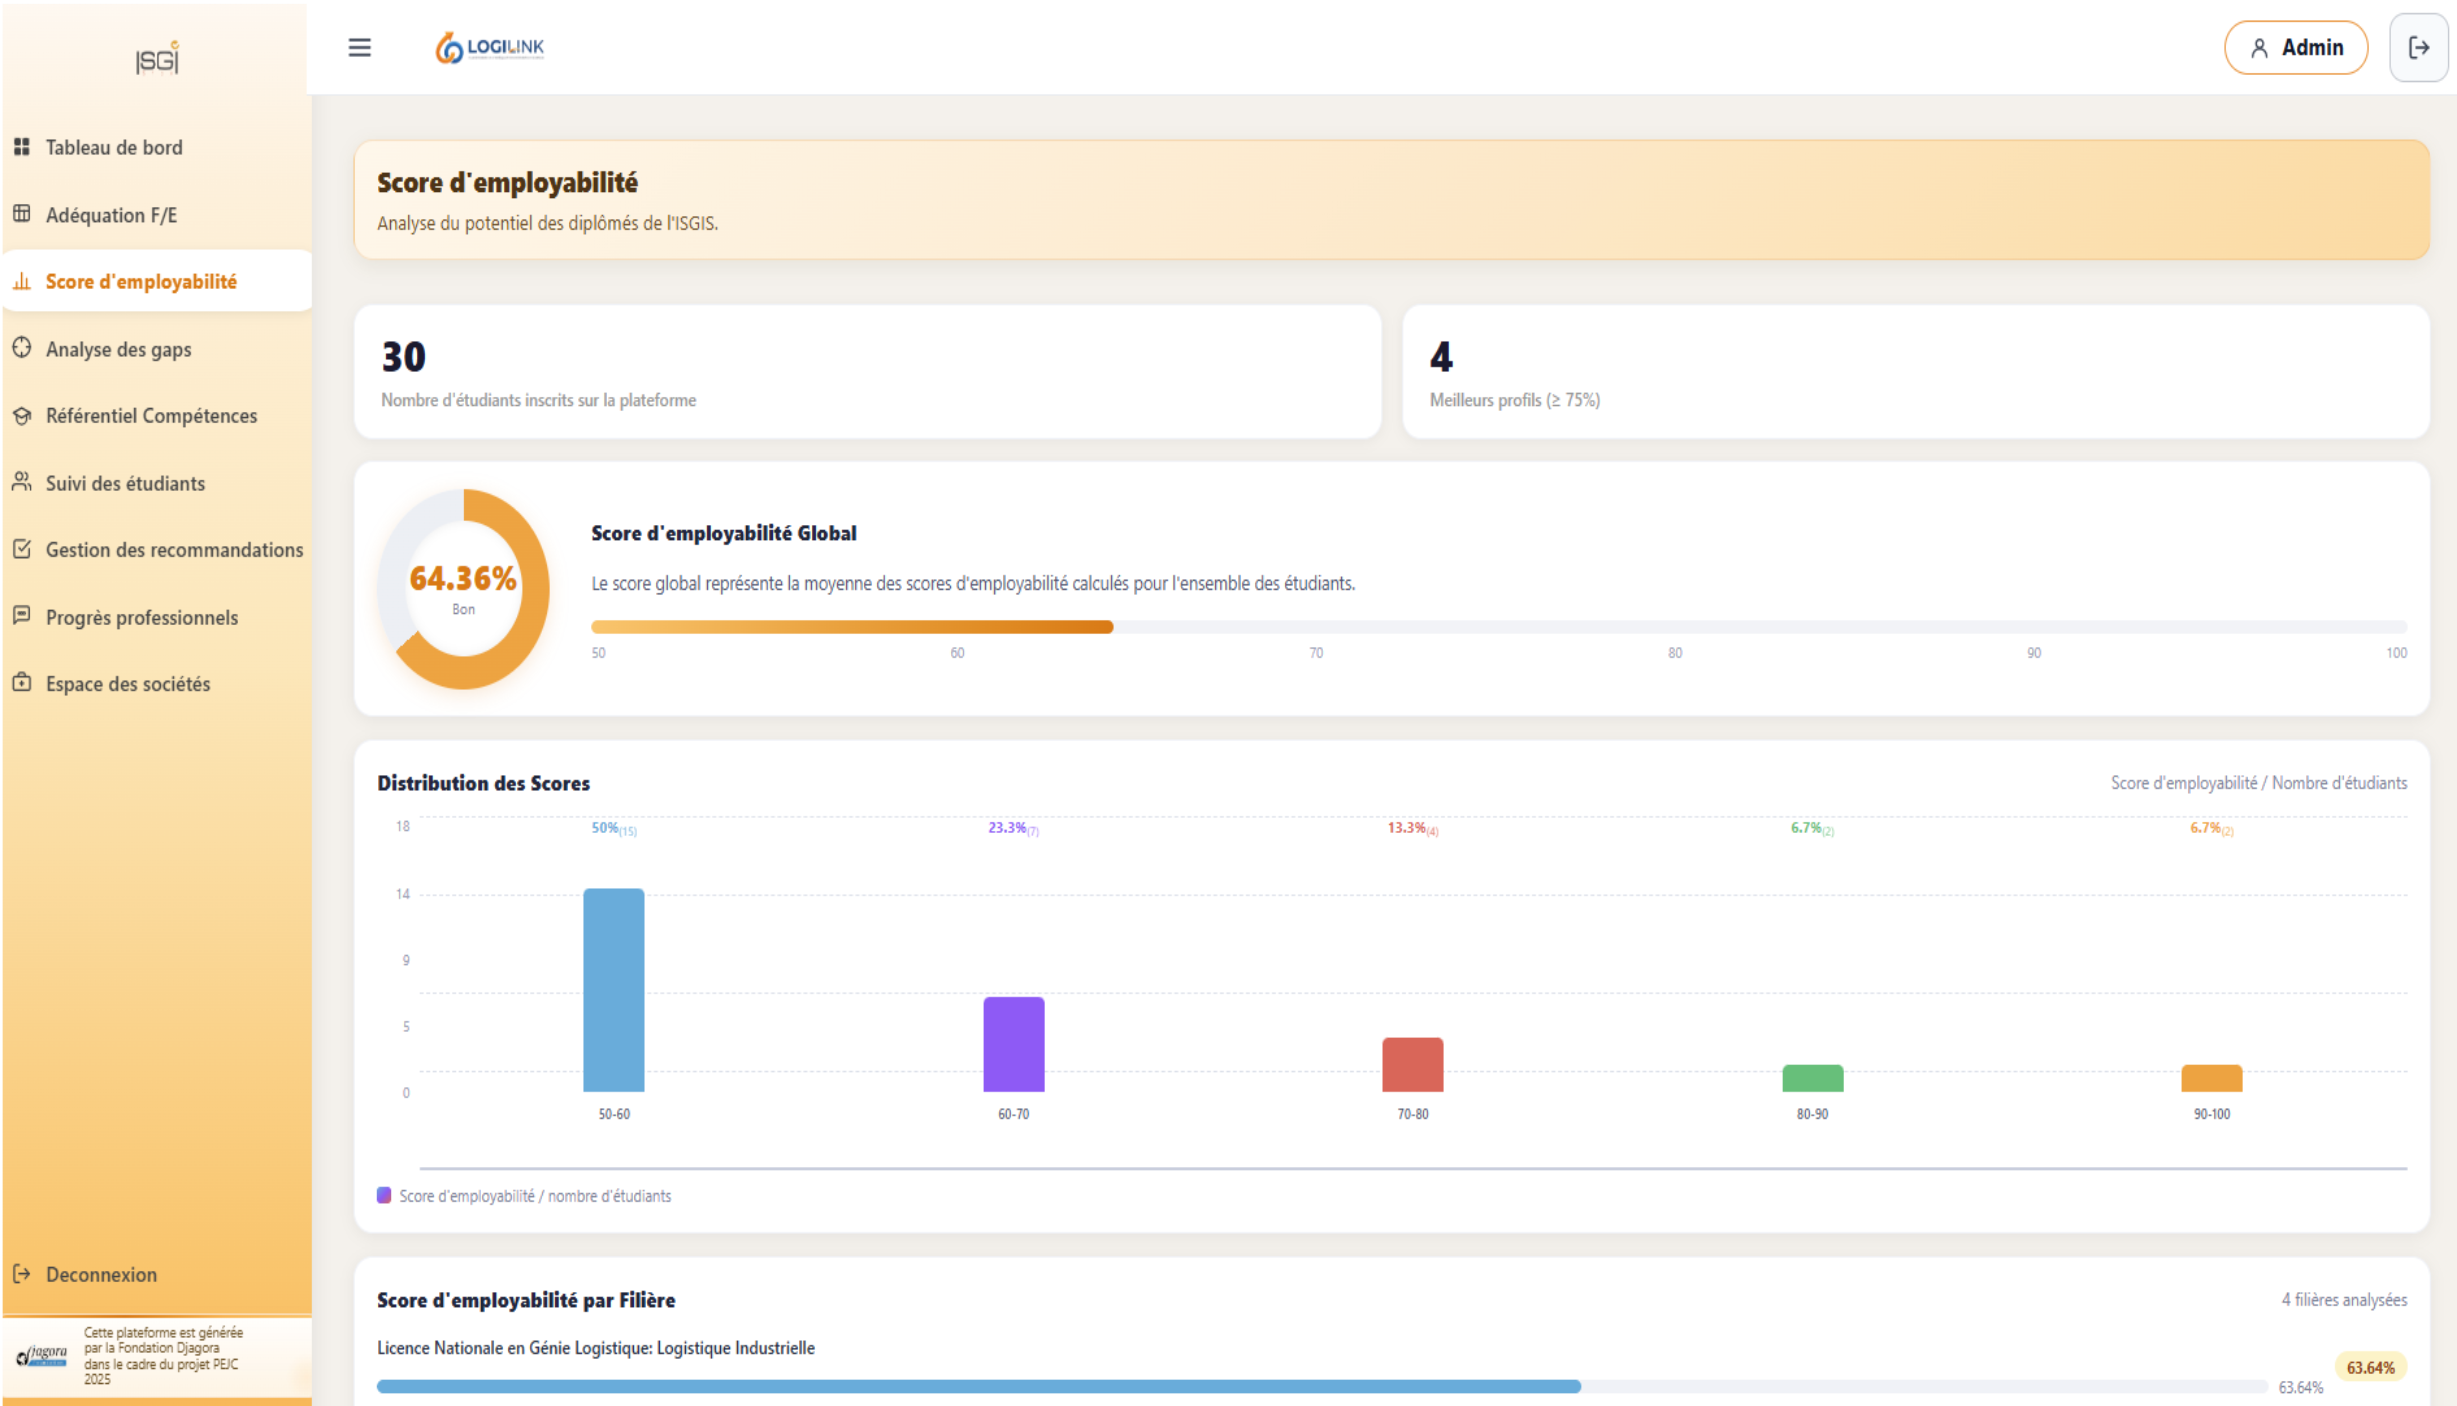
\includegraphics[width=0.85\textwidth]{figures/Interface_du_score_daemployabilite.png}
\caption{Interface du score d'employabilité}
\label{fig:score-employabilite}
\end{figure}

\begin{figure}[H]
\centering
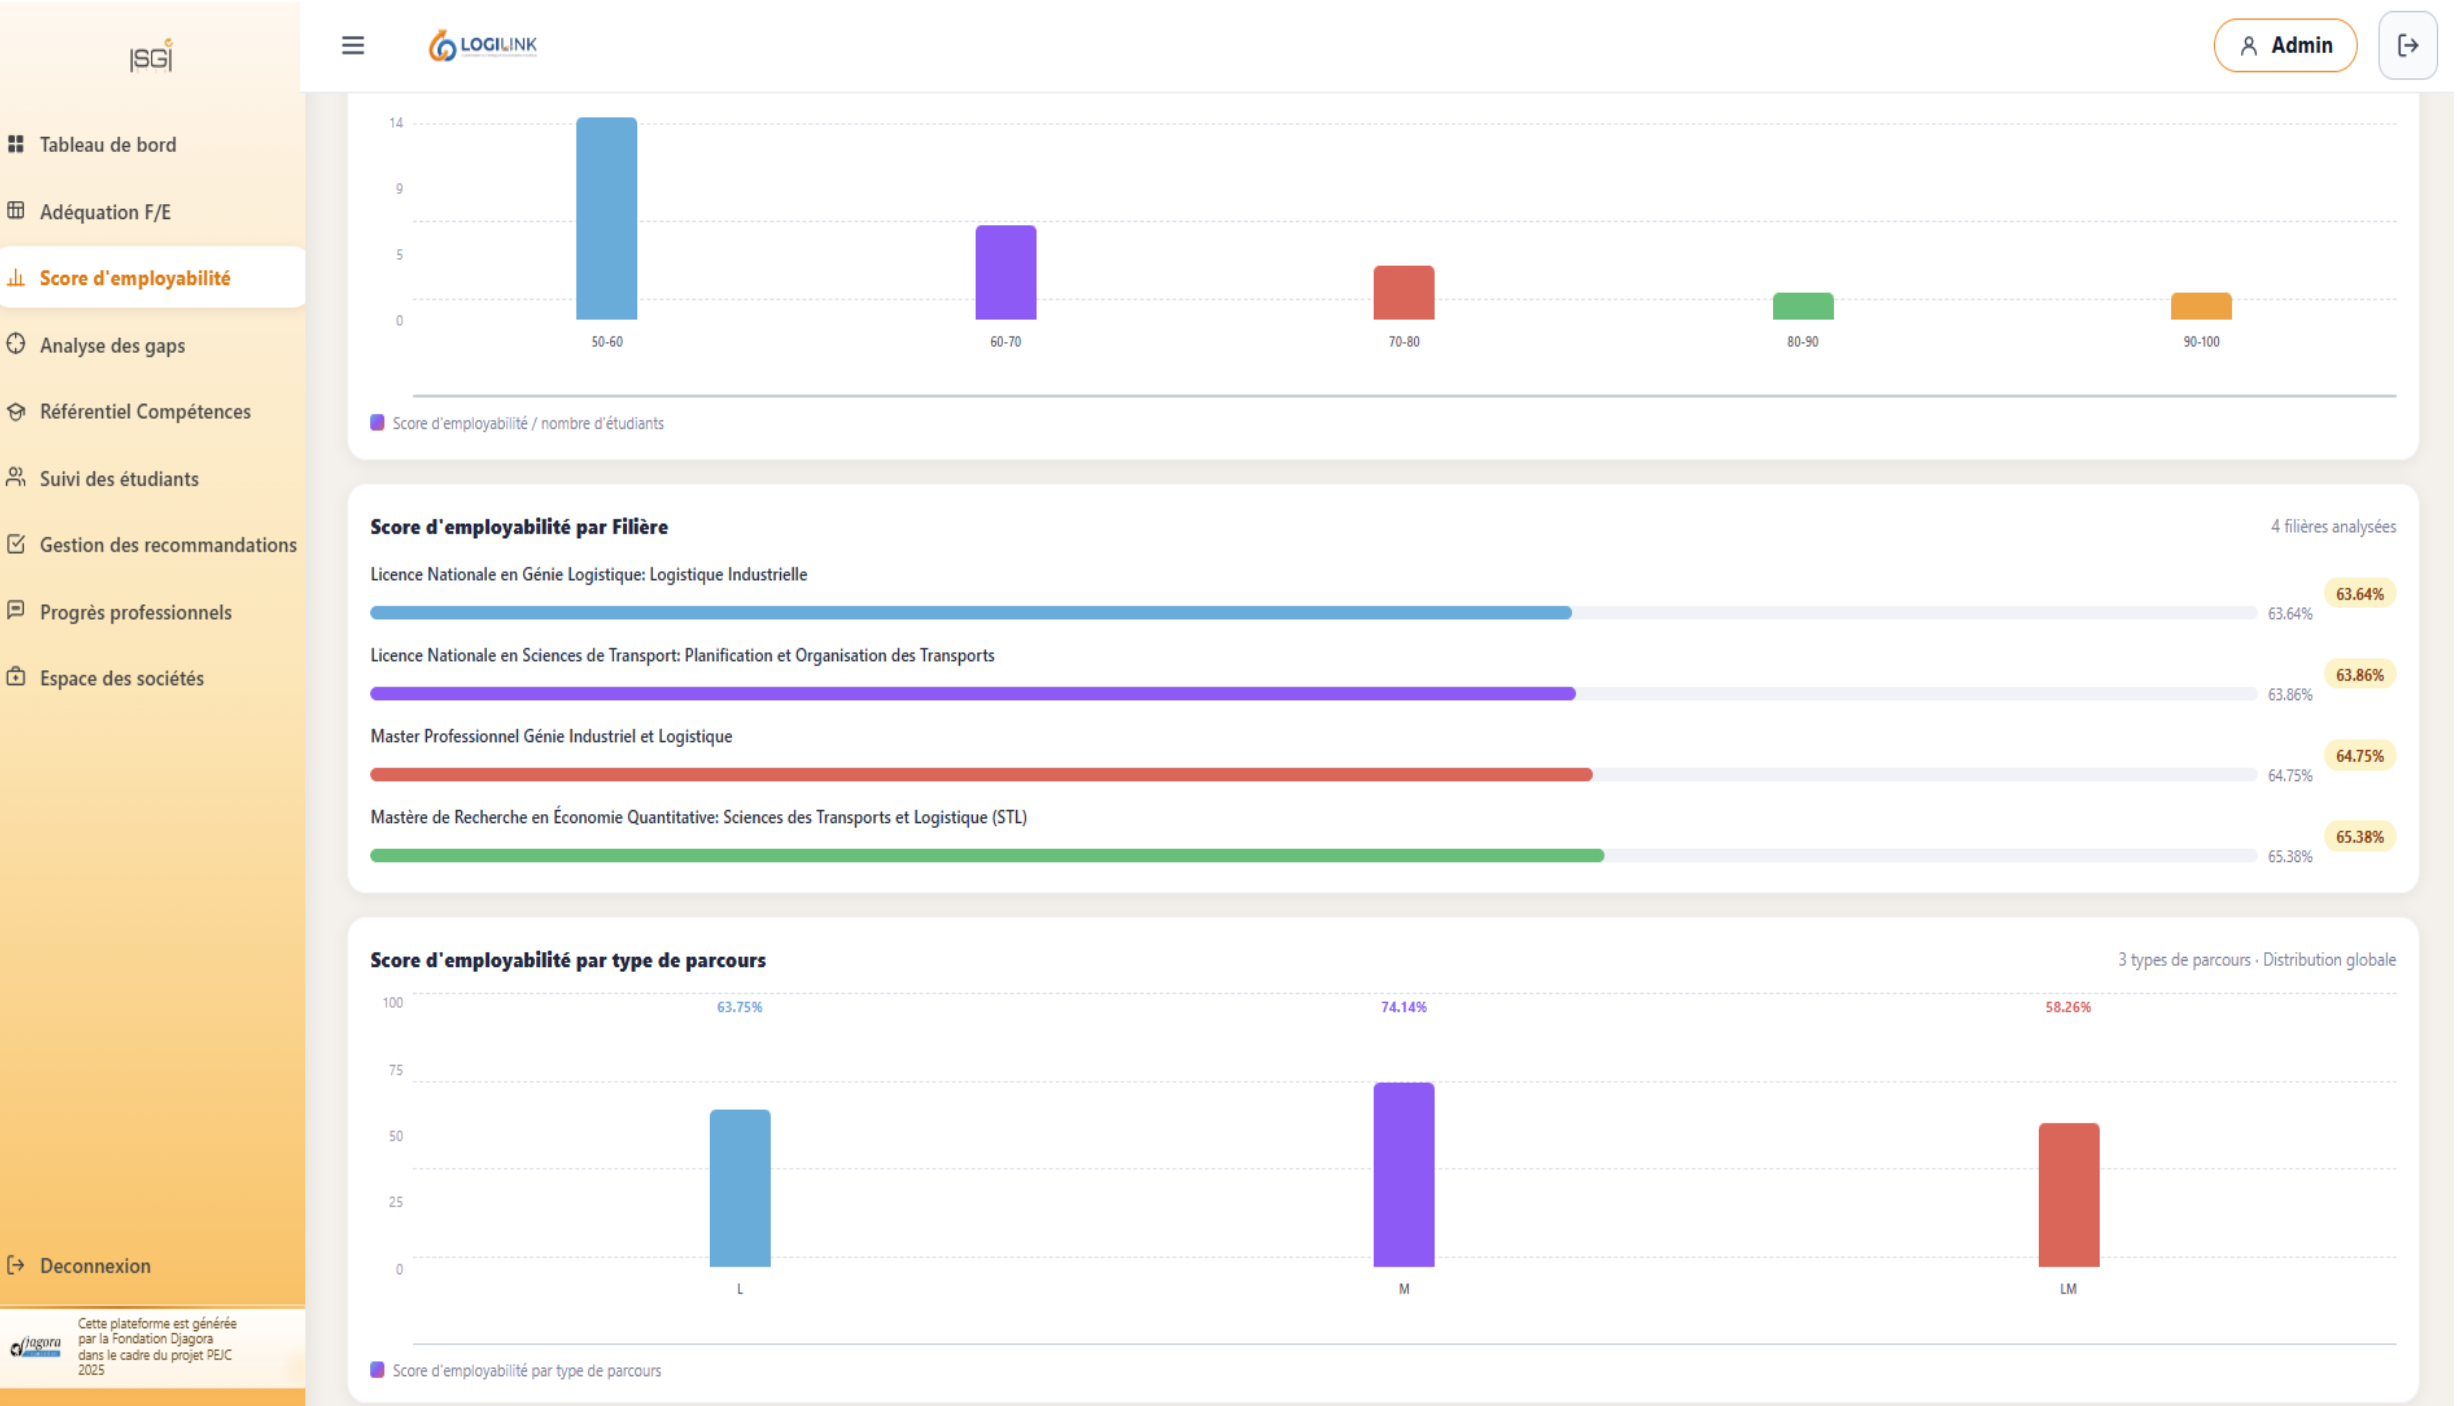
\includegraphics[width=0.85\textwidth]{figures/Interface_du_score_daemployabilite_2.png}
\caption{Interface du score d'employabilité}
\label{fig:score-employabilite-2}
\end{figure}

\noindent La figure~\ref{fig:adequation-formation-emploi} ci-dessous présente l'interface d'adéquation Formation-Emploi, qui permet d'analyser la correspondance entre les matières enseignées et les métiers. Elle intègre une matrice de couverture des compétences pouvant être filtrée par parcours et par filière. Chaque cellule de la matrice est associée à un coefficient variant de 0 à 1 (0 ; 0,2 ; 0,4 ; 0,6 ; 0,8 ; 1), indiquant le niveau de contribution de la matière au métier concerné.

\begin{figure}[H]
\centering
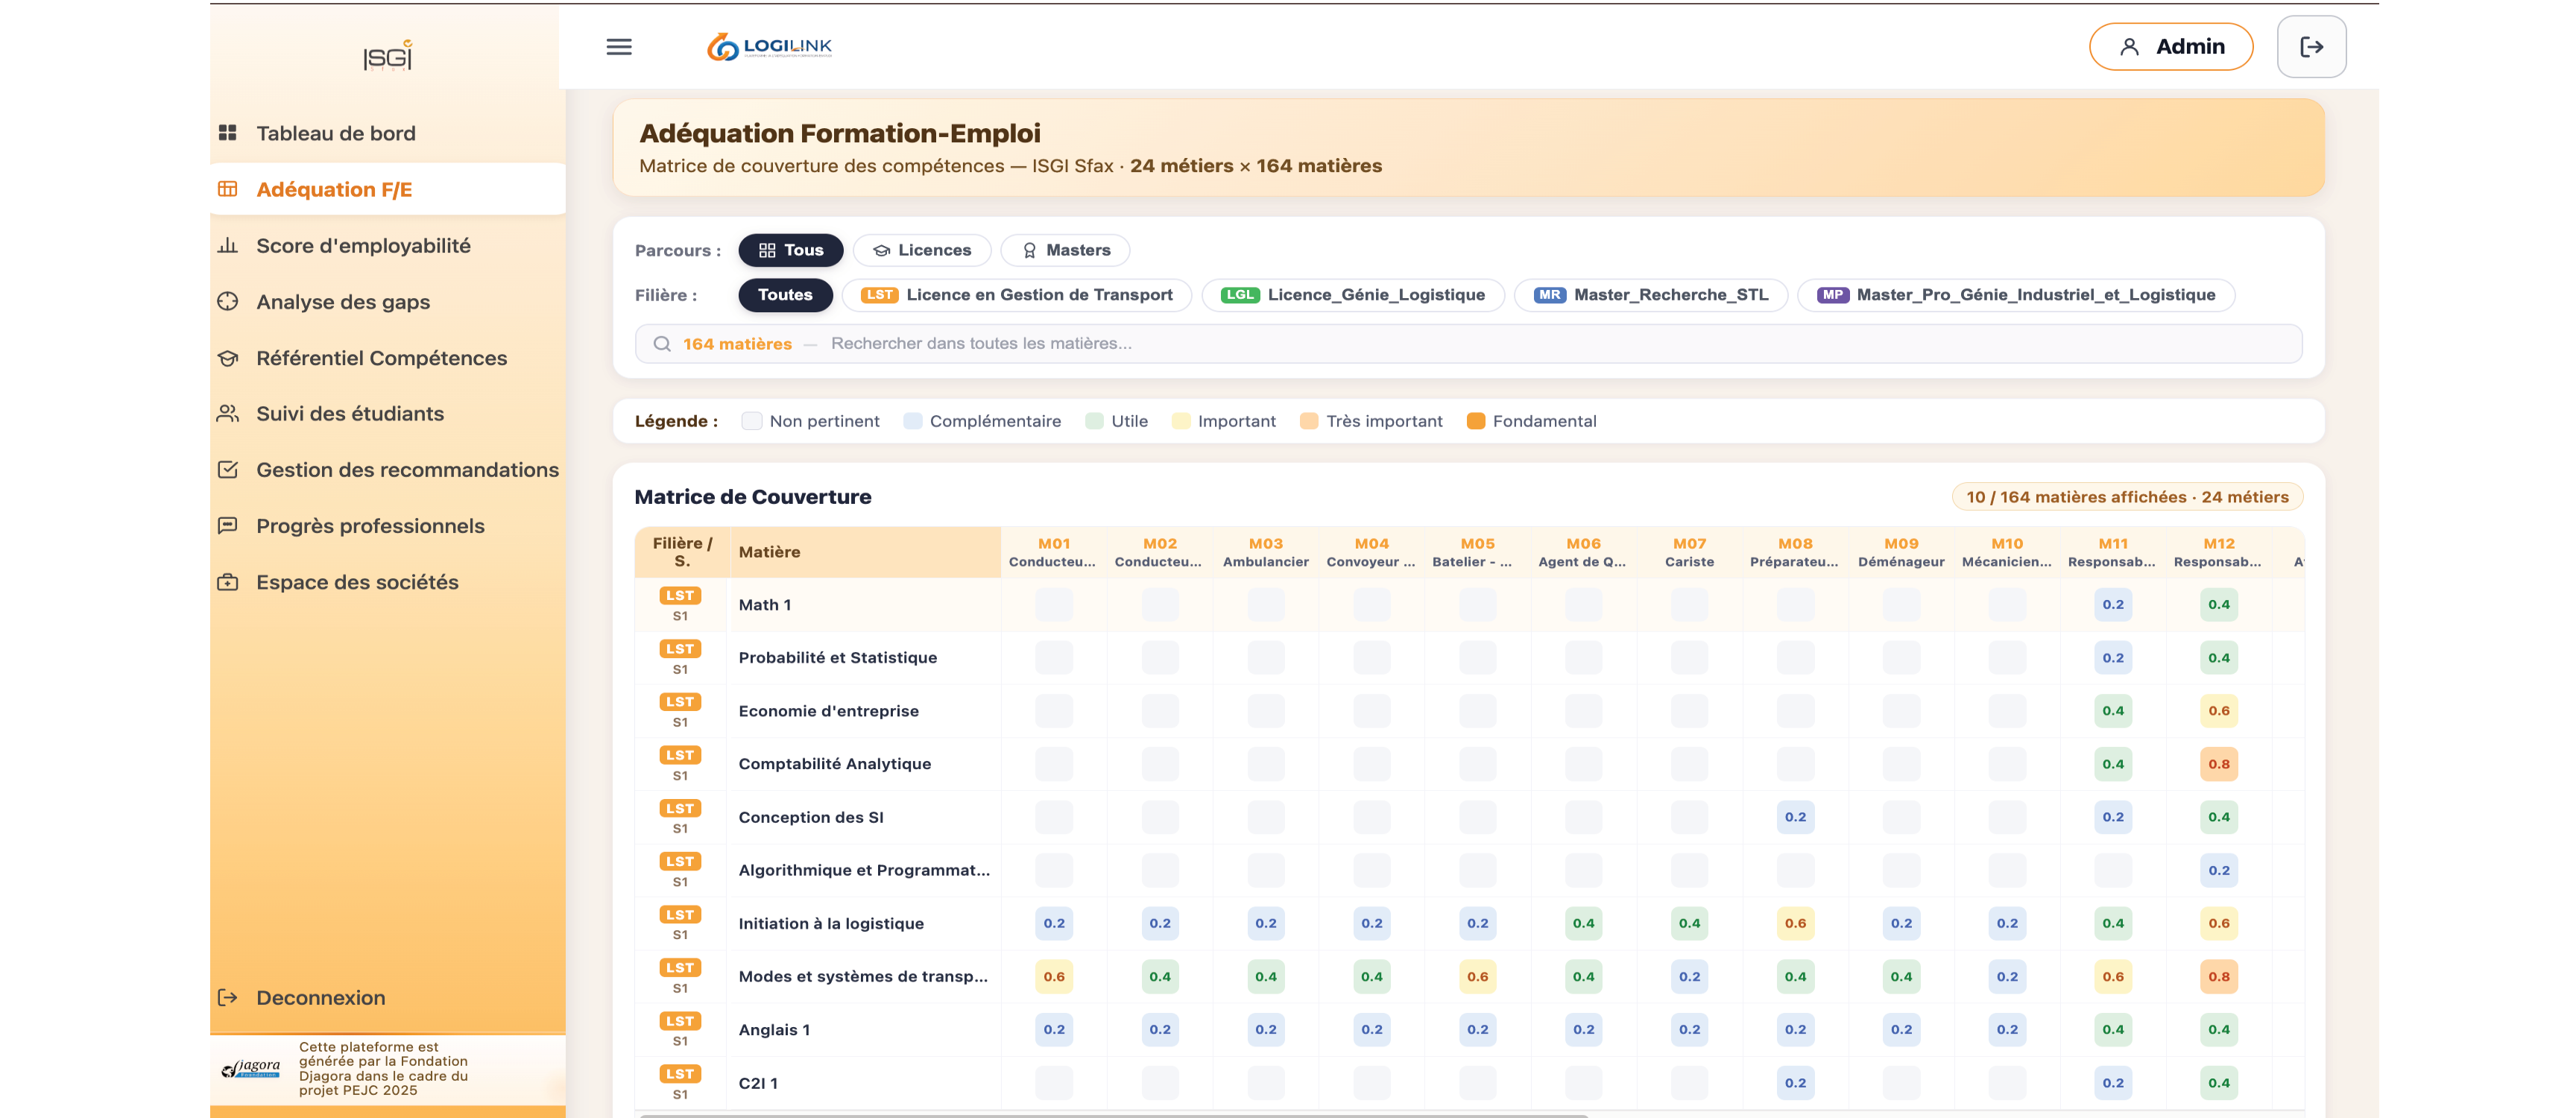
\includegraphics[width=0.85\textwidth]{figures/Interface_daadequation_Formation-Emploi.png}
\caption{Interface d'adéquation Formation-Emploi}
\label{fig:adequation-formation-emploi}
\end{figure}

\noindent La figure~\ref{fig:referentiel-competences} ci-dessous présente l'interface Référentiel Compétences, qui englobe l'ensemble des compétences par métiers dans le secteur Transport \& Logistique. Ces compétences sont classées par catégorie (techniques, organisationnelles, physiques et comportementales) ainsi que par domaine.

\begin{figure}[H]
\centering
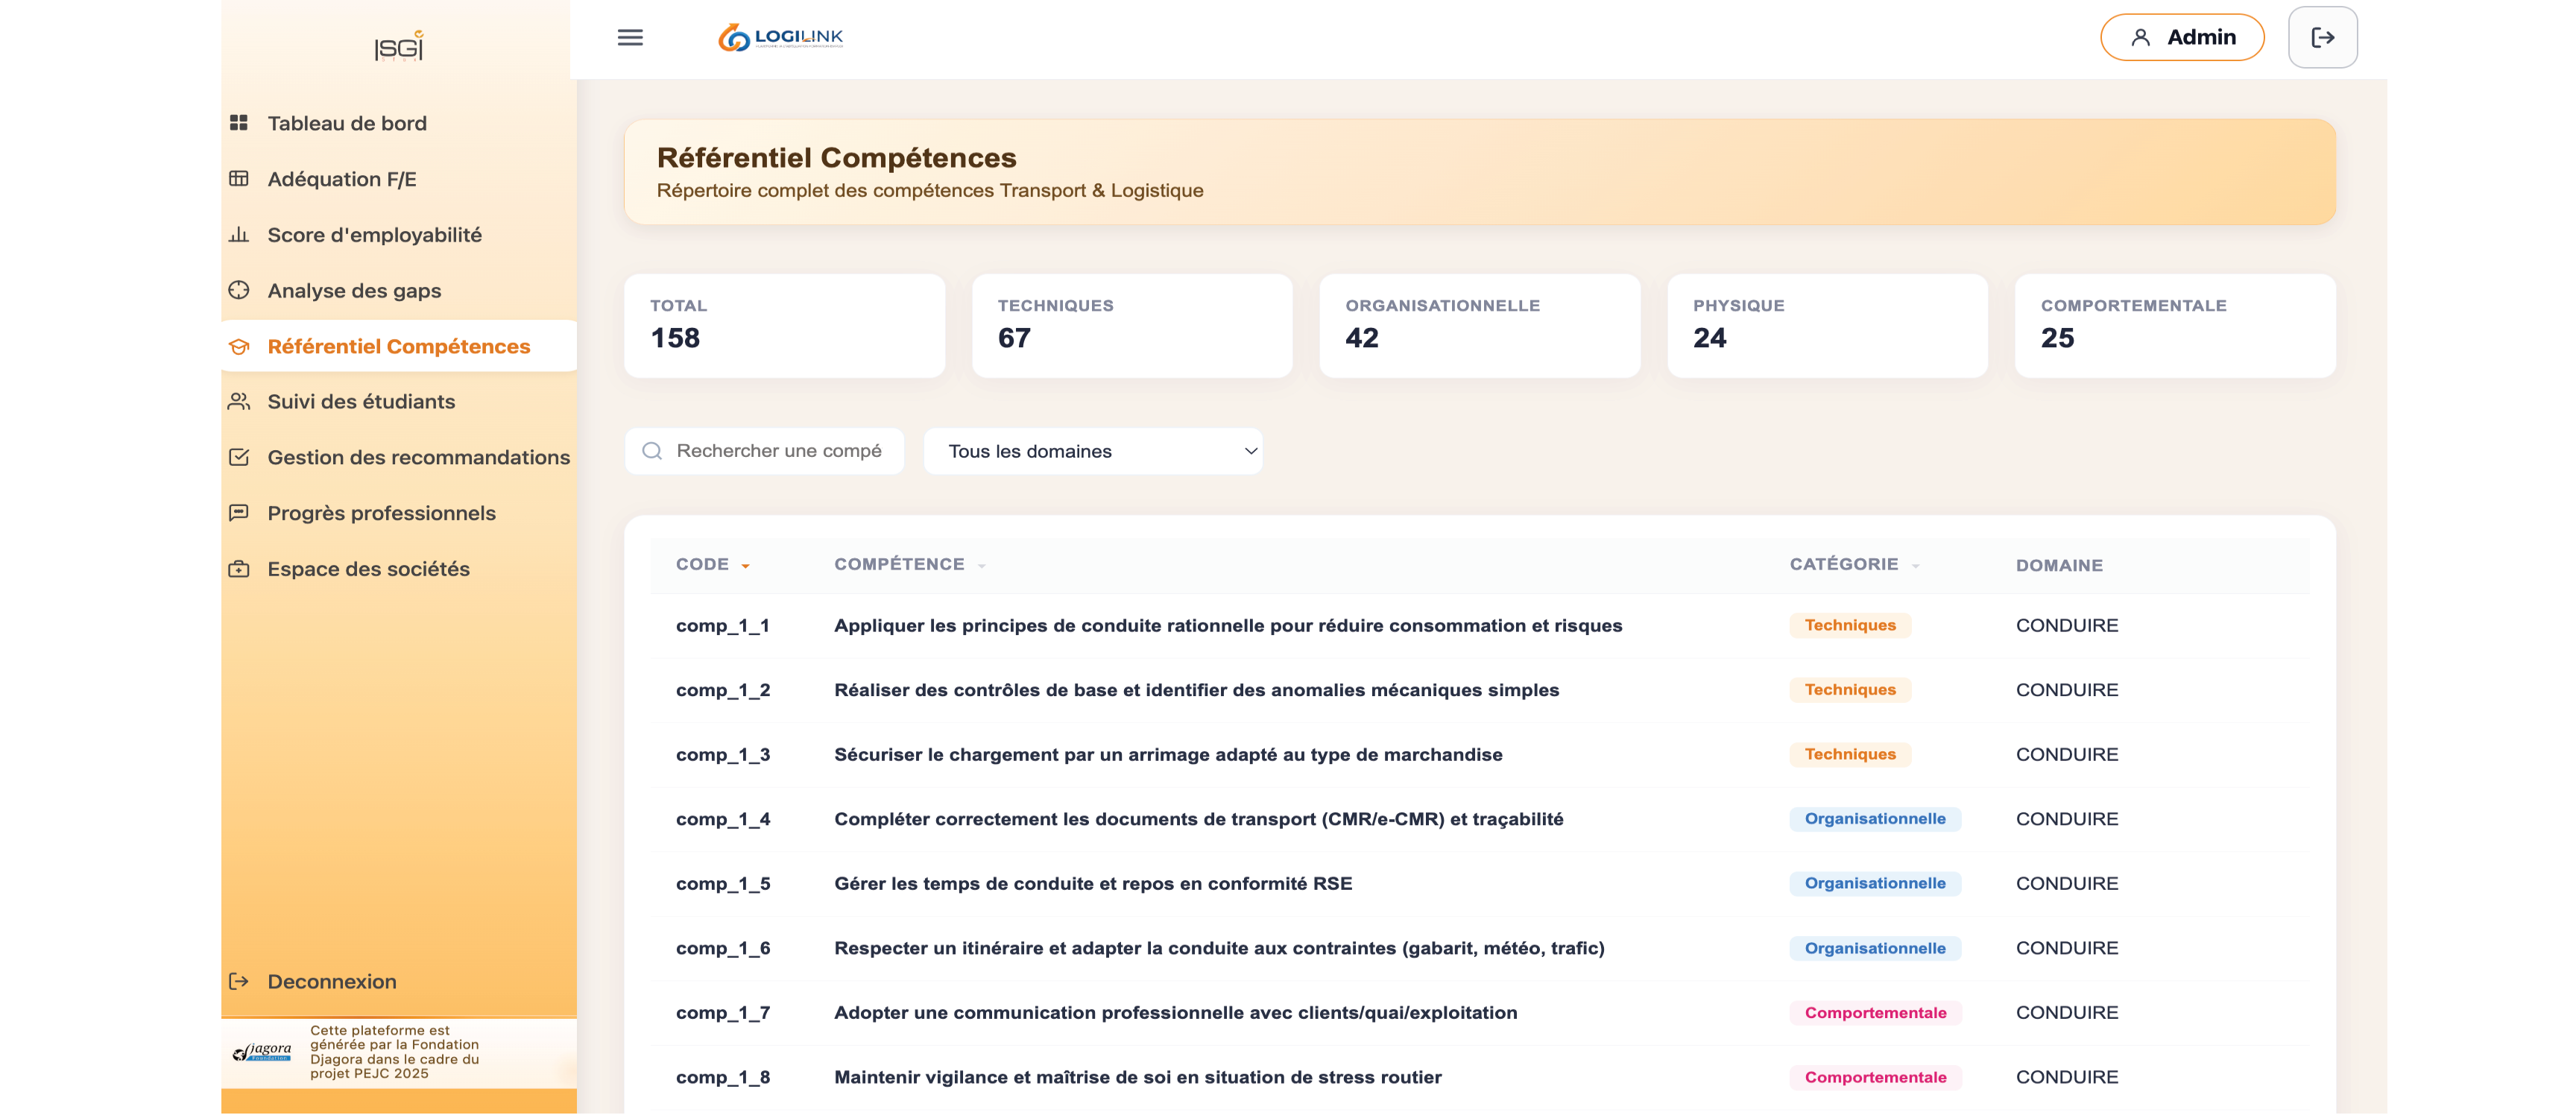
\includegraphics[width=0.85\textwidth]{figures/Interface_du_referentiel_des_competences.png}
\caption{Interface du référentiel des compétences}
\label{fig:referentiel-competences}
\end{figure}

\noindent La figure~\ref{fig:suivi-etudiants-filiere} ci-dessous présente l'interface Suivi des étudiants, ainsi que leur score CV ATS et leur score d'employabilité.

\begin{figure}[H]
\centering
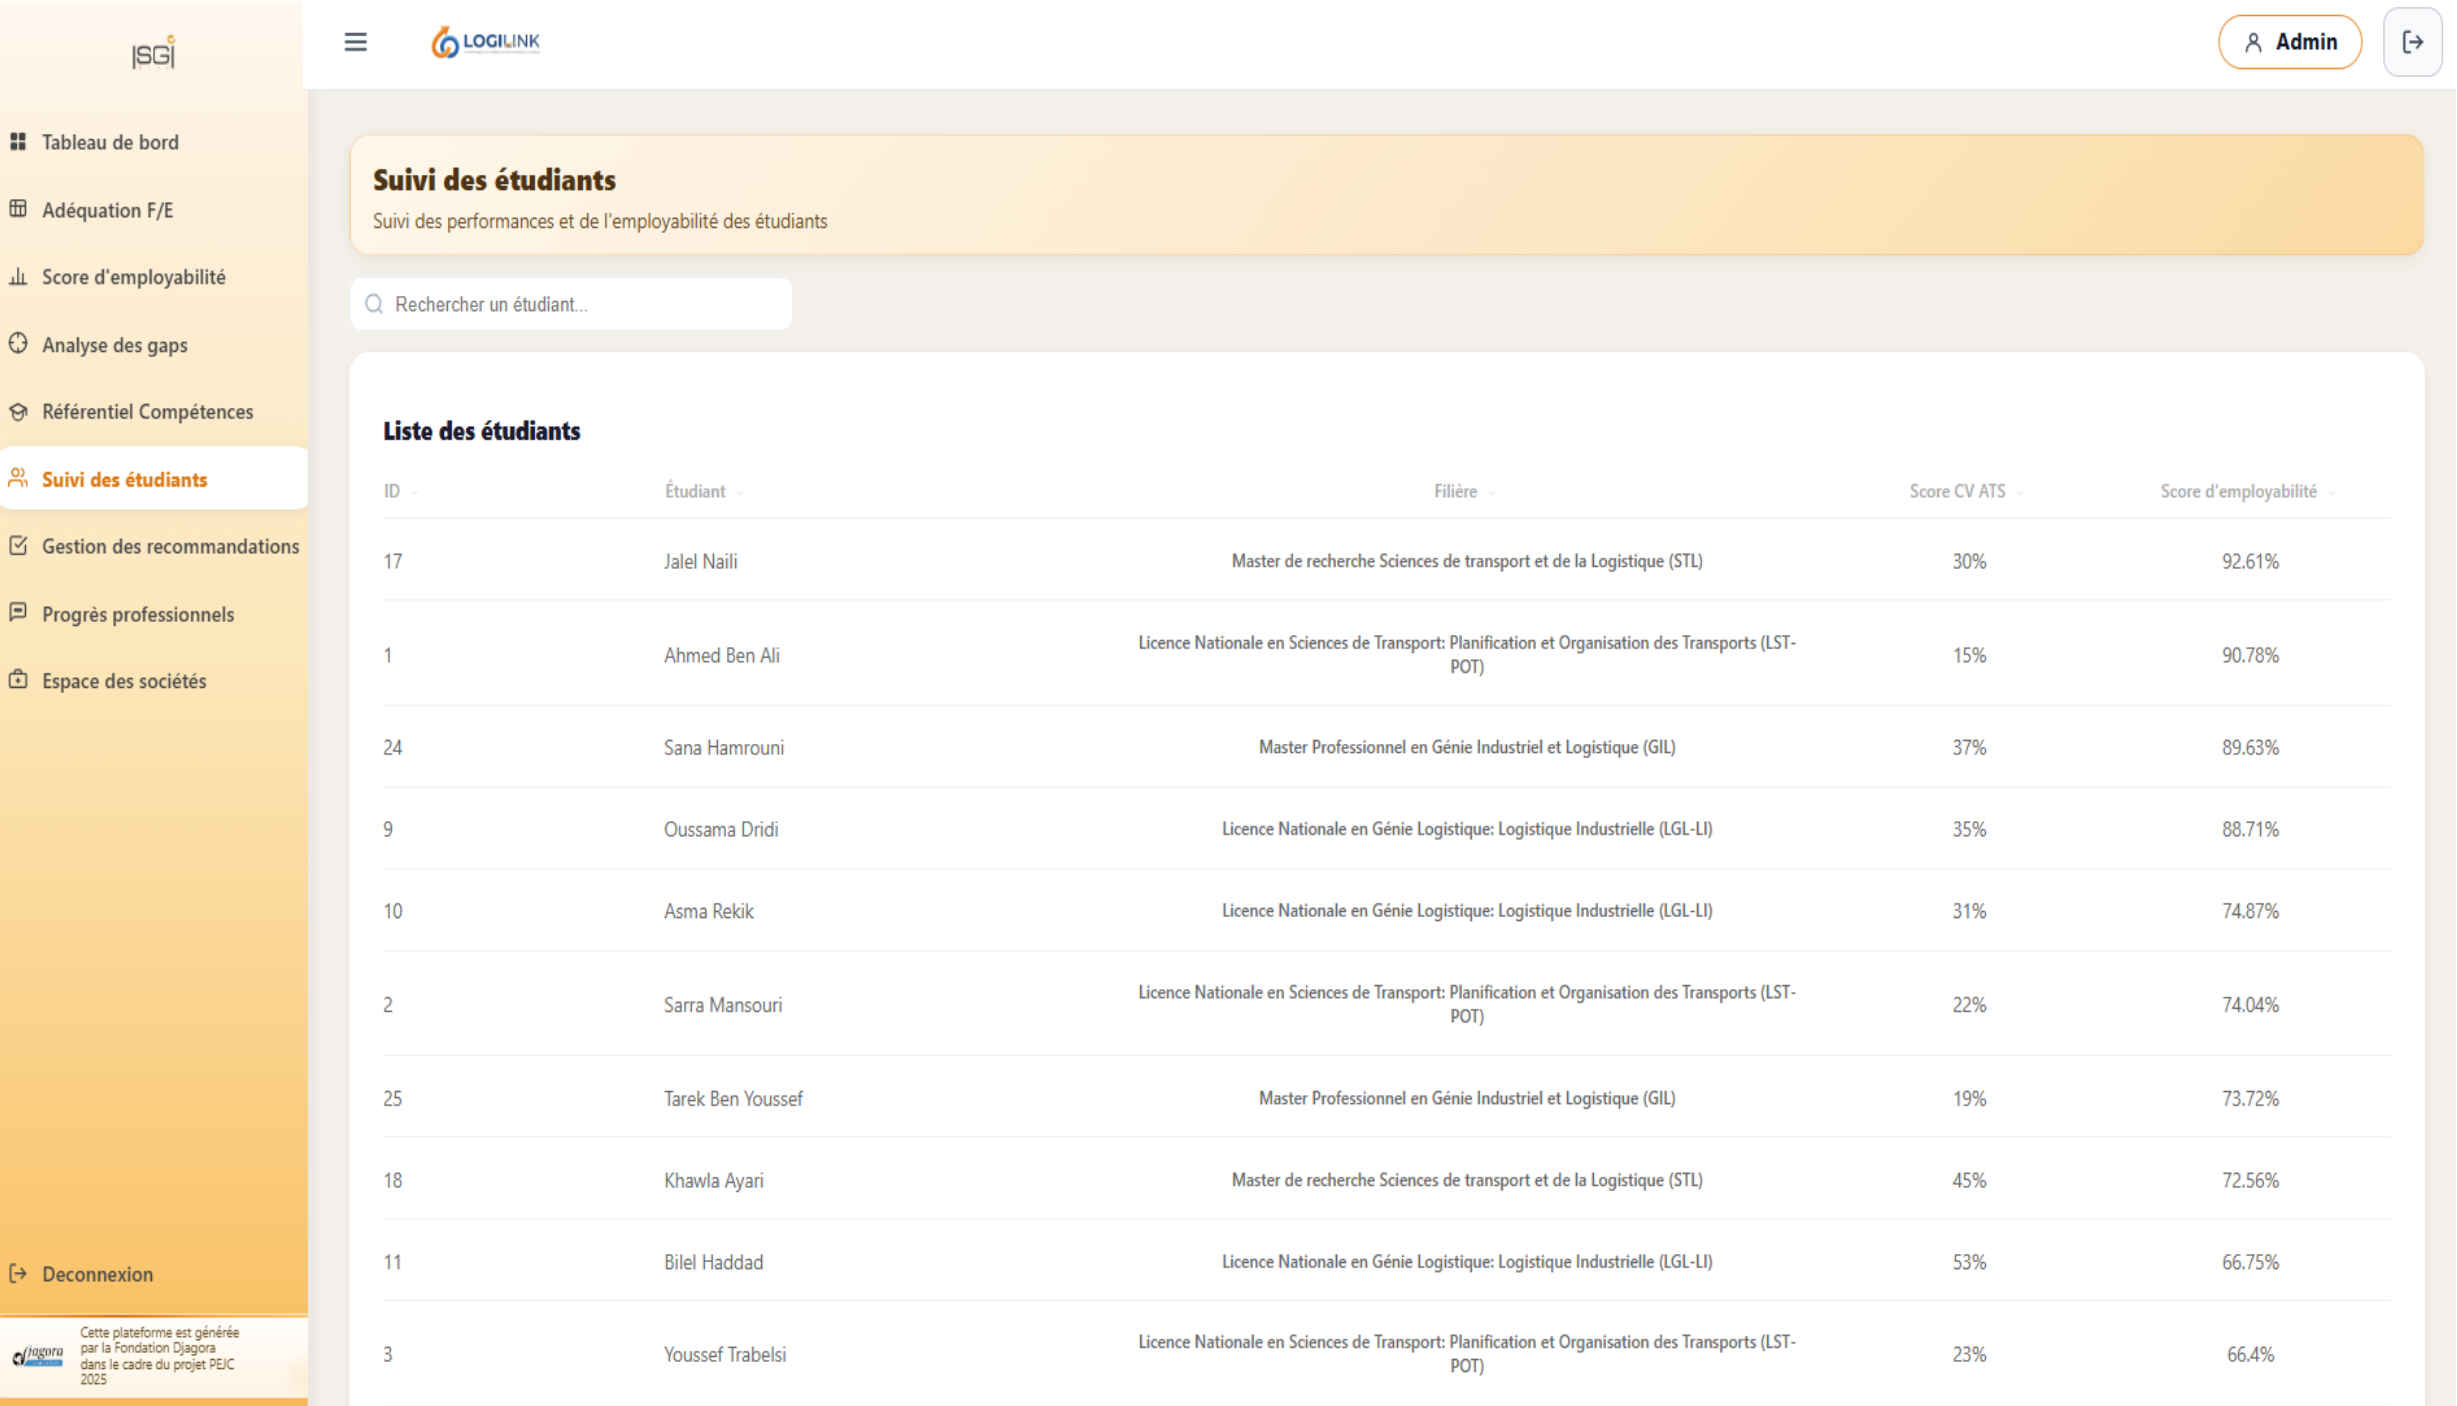
\includegraphics[width=0.85\textwidth]{figures/Interface_de_suivi_des_etudiants_par_filiere.png}
\caption{Interface de suivi des étudiants par filière}
\label{fig:suivi-etudiants-filiere}
\end{figure}

\subsection{Interfaces société}

La figure~\ref{fig:consultation-candidatures} ci-dessous permet à la société de consulter le score d'employabilité ainsi que le CV ATS de l'étudiant ayant postulé à une offre.

\begin{figure}[H]
\centering
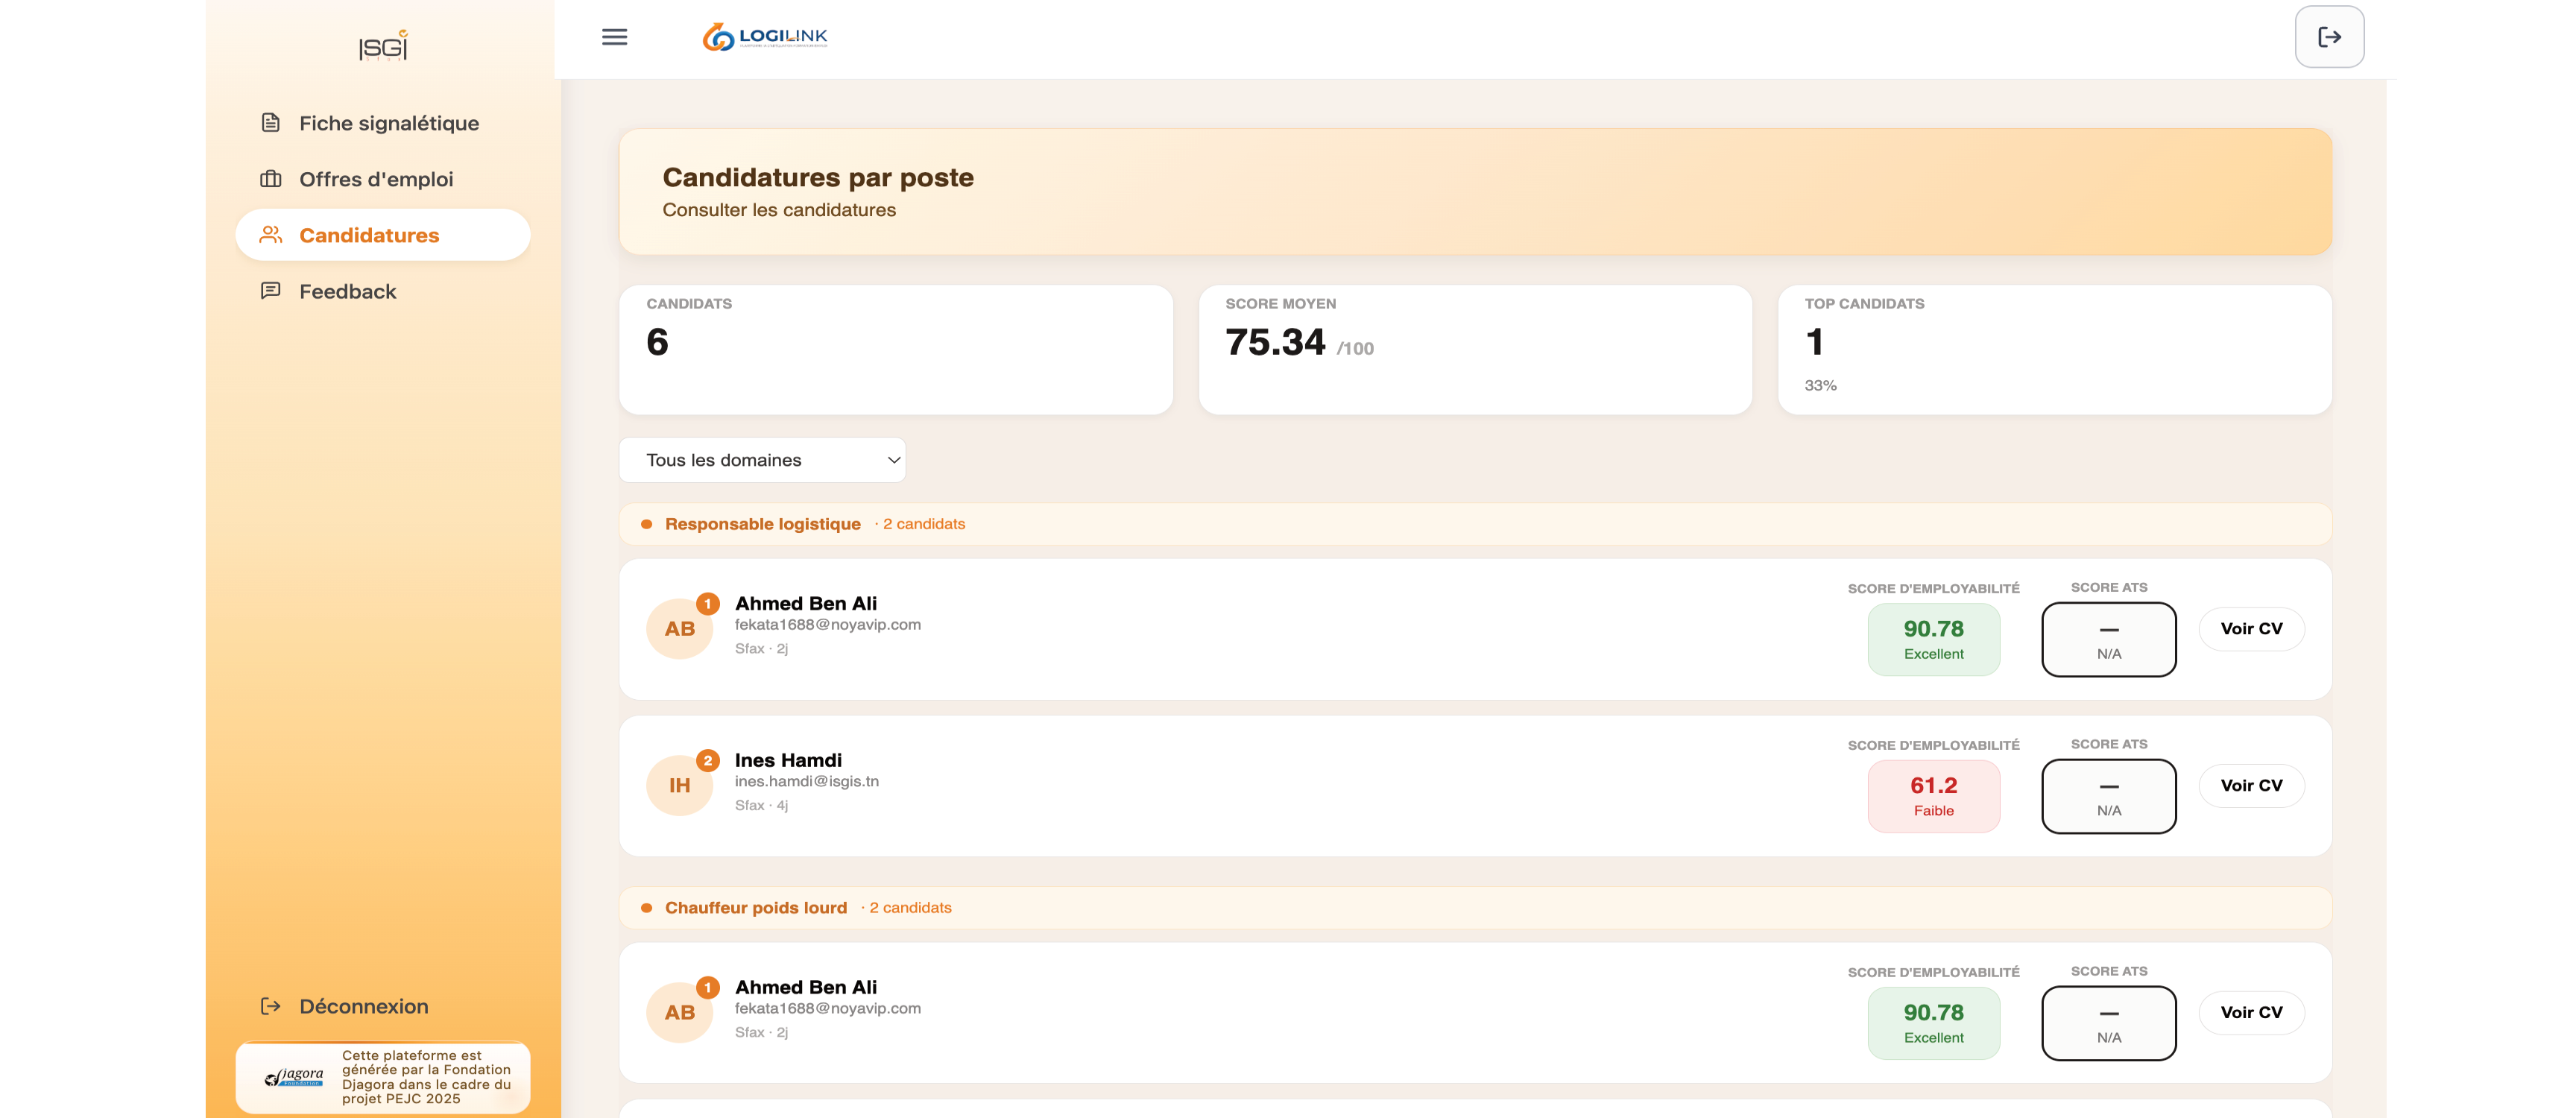
\includegraphics[width=0.85\textwidth]{figures/Interface_de_consultation_des_candidatures.png}
\caption{Interface de consultation des candidatures}
\label{fig:consultation-candidatures}
\end{figure}

\section{Conclusion}

Ce chapitre présente les environnements matériel et logiciel mis en place pour la réalisation du système, ainsi que les principales technologies adoptées pour son développement. L'environnement logiciel s'appuie sur des outils adaptés au travail collaboratif et au développement, tels que Visual Studio Code et GitHub, et sur un ensemble de technologies couvrant les différents besoins de la solution, par exemple Python pour le traitement et l'analyse des données, Node.js / NestJS pour la couche backend, Angular / TypeScript pour l'interface web, ainsi que MongoDB et Supabase (PostgreSQL) pour la gestion et le stockage des données.

\noindent Enfin, les interfaces développées ont permis de rendre le système accessible et facile à exploiter, en s'adaptant aux besoins de chaque profil (étudiant, administrateur et société). Elles proposent une navigation claire et des tableaux de bord facilitant la consultation des informations, tout en assurant une expérience utilisateur cohérente.
